\section{波导与谐振腔}
\subsection{金属波导综述}
\subsubsection{理想波导中的电磁波}
在大多数情形下，波导或谐振腔在某一方向的特征长度远大于其他方向，进而在麦克斯韦方程组中，可按纵向（即近乎无限延伸的方向 \(\uv{z}\)）、横向（即垂直于 \(\uv{z}\) 的方向，以下标 \(t = \text{transverse}\) 表示）分量展开.
假设电磁场按 \(e^{-i\omega t}\) 时谐因子振荡，以下 \(\vb{E}, \vb{H}\) 代表略去时谐因子的振幅.
在介电常数 \(\varepsilon\) 和磁导率 \(\mu\) 为常数的介质中
\begin{equation*}
	\nabla \times \vb{E} = i\omega\mu \vb{H}. \quad \nabla \times \vb{H} = -i\omega\varepsilon \vb{E}. \quad \nabla \cdot \vb{H} = 0. \quad \nabla \cdot \vb{E} = 0.
\end{equation*}

将电磁场及梯度算符按横向和纵向分量展开
\begin{equation*}
	\vb{E} = \vb{E}_t + \vb{E}_z. \quad \vb{H} = \vb{H}_t + \vb{H}_z. \quad \nabla = \nabla_t + \uv{z} \dfrac{\partial}{\partial z}.
\end{equation*}
其中 \(\vb{E}_z = \uv{z} (\uv{z} \cdot \vb{E}) = \uv{z} E_z\)，\(\vb{E}_t = (\uv{z} \times \vb{E}) \times \uv{z}\)，磁场同理.

麦克斯韦方程等价为
\begin{equation*}
	\dfrac{\partial \vb{E}_t}{\partial z} + i\omega\mu \uv{z} \times \vb{H}_t = \nabla_t E_z. \quad \uv{z} \cdot (\nabla_t \times \vb{E}_t) = i\omega\mu H_z.
\end{equation*}
\begin{equation*}
	\dfrac{\partial \vb{H}_t}{\partial z} - i\varepsilon\omega \uv{z} \times \vb{E}_t = \nabla_t H_z. \quad \uv{z} \cdot (\nabla_t \times \vb{H}_t) = -i\varepsilon\omega E_z.
\end{equation*}
\begin{equation*}
	\nabla_t \cdot \vb{E}_t = -\dfrac{\partial E_z}{\partial z}. \quad \nabla_t \cdot \vb{H}_t = -\dfrac{\partial H_z}{\partial z}.
\end{equation*}

数学简洁起见，只考虑波导沿 \(z\) 方向均匀延伸、横向截面形状不变的情况，此时电磁场在 \(z\) 方向以 \(e^{\pm ikz}\) 因子传播，振幅仅是横向坐标的函数.记 \(\gamma^2 = \mu\varepsilon\omega^2 - k^2\)，下只考虑非衰减、非平庸的横向模式，即要求 \(\gamma^2 > 0\)，事实上 \(\gamma = 0\) 常被称为截止之处 (cutoff)，其对应的 \(\omega\)、\(k\) 常被冠以截止之名.

代入 \(\gamma\)，由上方程组得
\begin{equation*}
	\vb{E}_t = \dfrac{i}{\gamma^2} \left( \nabla_t \dfrac{\partial E_z}{i\partial z} - \omega\mu \uv{z} \times \nabla_t H_z \right). \quad \vb{H}_t = \dfrac{i}{\gamma^2} \left( \nabla_t \dfrac{\partial H_z}{i\partial z} + \varepsilon\omega \uv{z} \times \nabla_t E_z \right).
\end{equation*}
\begin{equation*}
	(\gamma^2 + \nabla_t^2) E_z = 0. \quad (\gamma^2 + \nabla_t^2) H_z = 0.
\end{equation*}

考虑电磁场在横向截面 \(A\) 上被线边界为 \(C\) 的良导体包围，规定 \(C\) 的法向 \(\uv{n}\) 由介质指向良导体内部，\(C\) 的切向 \(\hat{\tau}\) 使得 \((\uv{n}, \hat{\tau}, \uv{z})\) 组成右手系基底（如图\ref{无限长波导示意图}），则边界条件给出
\begin{equation*}
	E_z \big|_C = 0. \quad \vb{E}_t \cdot \hat{\tau} = \dfrac{i}{\gamma^2} \left( \nabla_t \dfrac{\partial E_z}{i\partial z} - \omega\mu \uv{z} \times \nabla_t H_z \right) \cdot \hat{\tau} = 0.
\end{equation*}
\begin{equation*}
	\vb{H}_t \cdot \uv{n} = \dfrac{i}{\gamma^2} \left( \nabla_t \dfrac{\partial H_z}{i\partial z} + \varepsilon\omega \uv{z} \times \nabla_t E_z \right) \cdot \uv{n} = 0.
\end{equation*}

故（注意，\(E_z \big|_C = 0\) 已经保证了 \(\dfrac{\partial E_z}{\partial \tau} \big|_C = 0\)）
\begin{equation*}
	E_z \big|_C = 0. \quad \dfrac{\partial H_z}{\partial n} \big|_C = 0.
\end{equation*}
可见，\(E_z\) 和 \(H_z\) 满足拉普拉斯型方程，本征函数相互正交.
\begin{notes}
	数学上，对于同一区域上的拉普拉斯方程 \((\nabla_t^2 + \lambda^2) \Phi = 0\)，记Dirichlet边界条件（即 \(\Phi \big|_C = 0\)，\(C\) 为区域边界）给出的本征值谱为 \(\{\lambda_{D,1} < \lambda_{D,2} < \dots\}\)，记Neumann边界条件（即 \(\partial \Phi/\partial n \big|_C = 0\)，\(\partial/\partial n\) 指法向导数）给出的本征值谱为 \(\{\lambda_{N,0} = 0 < \lambda_{N,1} < \lambda_{N,2} < \dots\}\)，则总有 \(\lambda_{D,m} > \lambda_{N,m}\)（\(m \in \mathbb{Z}^+\)）.这将给出TE模式和TM模式的本征值的分布特点.
\end{notes}

不妨用 \(\lambda\) 代表本征模式序数，考虑到能量传播方向及电磁场无源条件，给出沿 \(\pm z\) 轴传播的电磁场形如
\begin{equation*}
	\vb{E}^{(\pm)} &= \sum_{\lambda} A_{\lambda}^{(\pm)} \vb{E}_{\lambda}^{(\pm)}(x, y, z) = \sum_{\lambda} A_{\lambda}^{(\pm)} \left( \vb{E}_{\lambda}(x, y) \pm \vb{E}_{z\lambda}(x, y) \right) e^{\pm i k_{\lambda} z}.\\
	\vb{H}^{(\pm)} &= \sum_{\lambda} A_{\lambda}^{(\pm)} \vb{H}_{\lambda}^{(\pm)}(x, y, z) = \sum_{\lambda} A_{\lambda}^{(\pm)} \left( \pm \vb{H}_{\lambda}(x, y) + \vb{H}_{z\lambda}(x, y) \right) e^{\pm i k_{\lambda} z}.
\end{equation*}
其中 \(A_{\lambda}^{(\pm)}\) 是振幅常数，\(\vb{E}_{\lambda}\) 和 \(\vb{H}_{\lambda}\) 为 \(\lambda\) 模式对应的横向电磁场，\(\vb{E}_{z\lambda} = E_{z\lambda} \uv{z}\) 和 \(\vb{H}_{z\lambda} = H_{z\lambda} \uv{z}\) 为 \(\lambda\) 模式对应的 \(z\) 方向电磁场.

总的电磁场则记为
\begin{equation*}
	\vb{E} = \vb{E}_t + \vb{E}_z = \sum_{\lambda} \left( A_{\lambda}^{(+)} e^{i k_{\lambda} z} + A_{\lambda}^{(-)} e^{-i k_{\lambda} z} \right) \vb{E}_{\lambda} + \sum_{\lambda} \left( A_{\lambda}^{(+)} e^{i k_{\lambda} z} - A_{\lambda}^{(-)} e^{-i k_{\lambda} z} \right) \vb{E}_{z\lambda}.
\end{equation*}
\begin{equation*}
	\vb{H} = \vb{H}_t + \vb{H}_z = \sum_{\lambda} \left( A_{\lambda}^{(+)} e^{i k_{\lambda} z} - A_{\lambda}^{(-)} e^{-i k_{\lambda} z} \right) \vb{H}_{\lambda} + \sum_{\lambda} \left( A_{\lambda}^{(+)} e^{i k_{\lambda} z} + A_{\lambda}^{(-)} e^{-i k_{\lambda} z} \right) \vb{H}_{z\lambda}.
\end{equation*}

将 \(\lambda\) 分为TE模式组和TM模式组，对应（记 \(Z = \sqrt{\mu/\varepsilon}\)）
\begin{equation*}
	\text{TM:}\quad& H_{z\lambda} = 0,\quad (\gamma_{\lambda}^2 + \nabla_t^2) E_{z\lambda} = 0,\quad E_{z\lambda} \big|_C = 0, \\
	&\vb{E}_{\lambda} = \dfrac{i k_{\lambda}}{\gamma_{\lambda}^2} \nabla_t E_{z\lambda}, \quad \vb{H}_{\lambda} = \dfrac{i k_{\lambda}}{\gamma_{\lambda}^2 Z_{\lambda}} \uv{z} \times \nabla_t E_{z\lambda}, \quad \dfrac{Z_{\lambda}}{Z} = \dfrac{k_{\lambda}}{\omega \sqrt{\varepsilon\mu}}.\\
	\text{TE:}\quad& E_{z\lambda} = 0,\quad (\gamma_{\lambda}^2 + \nabla_t^2) H_{z\lambda} = 0,\quad \dfrac{\partial H_{z\lambda}}{\partial n} \bigg|_C = 0, \\
	&\vb{E}_{\lambda} = -\dfrac{i k_{\lambda}}{\gamma_{\lambda}^2} Z_{\lambda} \uv{z} \times \nabla_t H_{z\lambda}, \quad \vb{H}_{\lambda} = \dfrac{i k_{\lambda}}{\gamma_{\lambda}^2} \nabla_t H_{z\lambda}, \quad \dfrac{Z_{\lambda}}{Z} = \dfrac{\omega \sqrt{\varepsilon\mu}}{k_{\lambda}}.
\end{equation*}

不难验证该分组方法满足横向场与纵向场的本构关系.

在实际求解中，\(E_{z\lambda}\) 或 \(H_{z\lambda}\) 可带有比例常数，为表述简洁起见，可规定不同模式间的归一化系数为

\begin{equation*}
	\lambda\in\text{TM:}\quad\int_A E_{z\lambda} E_{z\mu}^* \d a = \dfrac{\gamma_{\lambda}^2}{k_{\lambda}^2} \delta_{\lambda\mu}.
\end{equation*}
\begin{equation*}
	\lambda\in\text{TE:}\quad\int_A H_{z\lambda} H_{z\mu}^* \d a = \dfrac{\gamma_{\lambda}^2}{Z_{\lambda}^2 k_{\lambda}^2} \delta_{\lambda\mu}.
\end{equation*}

进而，不难验证
\begin{equation*}
	\int_A \vb{E}_{\lambda} \cdot \vb{E}_{\mu}^* \d a = \delta_{\lambda\mu}, \quad \int_A \vb{H}_{\lambda} \cdot \vb{H}_{\mu}^* \d a = \dfrac{1}{Z_{\lambda}^2} \delta_{\lambda\mu},\quad \dfrac{1}{2} \int_A \vb{E}_{\lambda} \times \vb{H}_{\mu}^* \cdot \uv{z} \, \d a = \dfrac{1}{2 Z_{\lambda}} \delta_{\lambda\mu}.
\end{equation*}

可见
\begin{equation*}
	A_{\lambda}^{(\pm)} &= \dfrac{1}{2} e^{\mp i k_{\lambda} z} \int_A \left( \vb{E}_{\lambda} \cdot \vb{E}_t \pm Z_{\lambda}^2 \vb{H}_{\lambda} \cdot \vb{H}_t \right) \d a.\\
	P^{(\pm)} &= \dfrac{1}{2} \int_A \Re\left[ \vb{E}_t^{(\pm)} \times \vb{H}_t^{(\pm)} \cdot \uv{z} \right] \d a = \sum_{\lambda} \dfrac{1}{2 Z_{\lambda}} \left| A_{\lambda}^{(\pm)} \right|^2.\\
	\dfrac{\d U^{(\pm)}}{\d z} &= \dfrac{\varepsilon}{4} \int_A \left( \left| \vb{E}^{(\pm)} \right|^2 + Z^2 \left| \vb{H}^{(\pm)} \right|^2 \right) \d a = \dfrac{\varepsilon}{2} \left( \sum_{\lambda \in \text{TM}} \dfrac{\omega^2 \mu\varepsilon}{k_{\lambda}^2} \left| A_{\lambda}^{(\pm)} \right|^2 + \sum_{\lambda \in \text{TE}} \left| A_{\lambda}^{(\pm)} \right|^2 \right).
\end{equation*}

在实际情况中，\(A_{\lambda}^{(\pm)}\) 应当由位于波导中的电流源激发，对于体积 \(V\) 内的电流密度分布 \(\vb{J}\)，由
\begin{equation*}
	\nabla \times \vb{E} = -\mu \dfrac{\partial \vb{H}}{\partial t}. \quad \nabla \times \vb{H} = \vb{J}. \quad \nabla \times \vb{E}_{\lambda} = -\mu \dfrac{\partial \vb{H}_{\lambda}}{\partial t}. \quad \nabla \times \vb{H}_{\lambda} = 0.
\end{equation*}
易得
\begin{equation*}
	\int_S \left( \vb{E} \times \vb{H}_{\lambda} - \vb{E}_{\lambda} \times \vb{H} \right) \cdot \uv{n}_S \, \d S = \int_V \vb{J} \cdot \vb{E}_{\lambda} \, \d \vb{r}.
\end{equation*}
其中 \(S\) 是包裹 \(V\) 的闭合曲面，\(\uv{n}_S\) 是曲面的外法向量，\(\d S\) 是关于 \(S\) 的面积元，\(\d \vb{r}\) 是关于 \(V\) 的体积元.

将 \(S\) 取为包裹侧壁的无限长柱面加上 \(z \to \pm\infty\) 无穷远处的波导截面，由
\begin{equation*}
	&\vb{E} \big|_{S_C} = \vb{E}_{\lambda} \big|_{S_C} = 0. \quad \uv{n}_S \times \vb{E} \big|_{z \to \pm\infty} = \pm \sum_{\lambda} A_{\lambda}^{(\pm)} \uv{z} \times \vb{E}_{\lambda}(x, y) e^{\pm i k_{\lambda} z}.\\
	&\uv{n}_S \times \vb{H} \big|_{z \to \pm\infty} = \sum_{\lambda} A_{\lambda}^{(\pm)} \uv{z} \times \vb{H}_{\lambda}(x, y) e^{\pm i k_{\lambda} z}.
\end{equation*}
积分得
\begin{equation*}
	A_{\lambda}^{(\pm)} = \dfrac{Z_{\lambda}}{2} \int_{\text{apt}} \left( \uv{n}_S \times \vb{E} \right) \cdot \vb{H}_{\lambda}^{(\mp)} \, \d S - \dfrac{Z_{\lambda}}{2} \int_V \vb{J} \cdot \vb{E}_{\lambda}^{(\mp)} \, \d \vb{r}.
\end{equation*}
其中，\(\text{apt}\) (aperture) 指侧壁上的小孔，\(\setminus\) 表示取差集.

若电流源和小孔非常小，可以将本征模式在源或孔的中心附近展开.运用以上 \(\vb{E}_{\lambda}\) 和 \(\vb{H}_{\lambda}\) 的关系式，并注意 \(\uv{n}_S \cdot \vb{r} = 0\)，展开两阶得
\begin{equation*}
	\int_V \vb{J} \cdot \vb{E}_{\lambda}^{(\mp)} \, \d \vb{r} &\approx \int \left( \vb{J} \cdot \vb{E}_{\lambda}^{(\mp)} \big|_{\text{sc}} + \vb{J} \cdot \left( \vb{r} \cdot \nabla \vb{E}_{\lambda}^{(\mp)} \big|_{\text{sc}} \right) \right) \d \vb{r} \\&= \dfrac{\partial \vb{p}_s}{\partial t} \cdot \vb{E}_{\lambda}^{(\mp)} \big|_{\text{sc}} - \vb{m}_s \cdot \mu \dfrac{\partial \vb{H}_{\lambda}^{(\mp)}}{\partial t} + \dfrac{1}{6} \dfrac{\partial \vb{D}_s}{\partial t} : \nabla \vb{E}_{\lambda}^{(\mp)} \big|_{\text{sc}}.\\
	\int_{\text{apt}} \left( \uv{n}_S \times \vb{E} \right) \cdot \vb{H}_{\lambda}^{(\mp)} \, \d S &\approx \int_{\text{apt}} \left( \left( \uv{n}_S \times \vb{E} \right) \cdot \vb{H}_{\lambda}^{(\mp)} \big|_{\text{ac}} + \left( \uv{n}_S \times \vb{E} \right) \cdot \left( \vb{r} \cdot \vb{H}_{\lambda}^{(\mp)} \right) \big|_{\text{ac}} \right) \d S \\&= \dfrac{1}{2} \left( \dfrac{\partial \vb{m}_a}{\partial t} \cdot \mu \vb{H}_{\lambda}^{(\mp)} \big|_{\text{ac}} - \vb{p}_a \cdot \dfrac{\partial \vb{E}_{\lambda}^{(\mp)}}{\partial t} \big|_{\text{ac}} + \dfrac{1}{6} \dfrac{\partial \vb{Q}_a}{\partial t} : \mu \nabla \vb{H}_{\lambda}^{(\mp)} \big|_{\text{ac}} \right).
\end{equation*}
其中下标 s (source) 表示源，sc (source center) 表示在源的中心处取值，a (aperture) 表示小孔，ac (aperture center) 表示在小孔的中心取值.

上式对应的特征电偶极矩、磁偶极矩、电四极矩、磁四极矩为
\begin{equation*}
	\vb{p}_s &= \int_V \rho \vb{r} \, \d \vb{r}. \quad \vb{m}_s = \int_V \dfrac{1}{2} \vb{r} \times \vb{J} \, \d \vb{r}. \quad \vb{D}_s = \int_V \rho \left( 3\vb{r}\vb{r} - r^2 \vb{I} \right) \d \vb{r}.\\
	\vb{p}_a &= \varepsilon \uv{n}_S \int_{\text{apt}} \vb{r} \cdot \vb{E} \, \d S. \quad \vb{m}_a = 2 \int_{\text{apt}} \vb{r} \left( \uv{n}_S \cdot \vb{H} \right) \d S. \quad \vb{Q}_a = 2 \int_{\text{apt}} \uv{n}_S \cdot \vb{H} \left( 3\vb{r}\vb{r} - r^2 \vb{I} \right) \d S.
\end{equation*}
其中 \(\vb{E}, \vb{H}\) 是小孔处的实际电磁场. 若小孔尺寸远小于电磁波波长，可以保留至最低阶辐射项，并在求解实际电磁场时忽略小孔的影响.

当场点位于波导内部时，\(\uv{n}_S = \uv{n}\).同理易证，当场点位于外部空间时，\(A_{\lambda}^{(\pm)}\) 不含与源有关的项，而小孔对 \(A_{\lambda}^{(\pm)}\) 的贡献同上，只不过 \(\uv{n}_S = -\uv{n}\)，且 \(\varepsilon, \mu\) 应当取外部空间的值.

综上，总的激发的振幅为
\begin{equation*}
	A_{\lambda}^{(\pm)} = &\dfrac{Z_{\lambda}}{2} \Bigg[ \dfrac{1}{2} \left( -\dfrac{\partial \vb{m}_a}{\partial t} \cdot \mu \vb{H}_{\lambda}^{(\mp)} \big|_{\text{ac}} + \vb{p}_a \cdot \dfrac{\partial \vb{E}_{\lambda}^{(\mp)}}{\partial t} \big|_{\text{ac}} - \dfrac{1}{6} \dfrac{\partial \vb{Q}_a}{\partial t} : \mu \nabla \vb{H}_{\lambda}^{(\mp)} \big|_{\text{ac}} \right)\\ &\quad+ \left( \dfrac{\partial \vb{p}_s}{\partial t} \cdot \vb{E}_{\lambda}^{(\mp)} \big|_{\text{sc}} - \vb{m}_s \cdot \mu \dfrac{\partial \vb{H}_{\lambda}^{(\mp)}}{\partial t}\big|_{\text{sc}} + \dfrac{1}{6} \dfrac{\partial \vb{D}_s}{\partial t} : \nabla \vb{E}_{\lambda}^{(\mp)} \big|_{\text{sc}} \right) \Bigg].
\end{equation*}
\begin{notes}
	%在第\ref{导体平面上的圆形孔}节，
	曾求出无限大导体平板上圆形小孔对空间电磁场的影响
	\begin{equation*}
		\vb{E} \big|_{\text{apt}} = E_0 \dfrac{\rho}{\pi \sqrt{a^2 - \rho^2}} \uv{\rho}. \quad \vb{H} \big|_{\text{apt}} = H_0 \left( \dfrac{1}{2} \left( \sin\phi \uv{\rho} + \cos\phi \uv{\phi} \right) + \dfrac{2\rho}{\pi \sqrt{a^2 - \rho^2}} \sin\phi \uv{z} \right).
	\end{equation*}
	其中 \(\vb{E}_0 = -E_0 \uv{z}\) 和 \(\vb{H}_0 = H_0 \uv{y}\) 是不存在小孔时的电磁场（显然，边界条件要求前者沿法向、后者沿切向），\(a\) 是小孔半径，\((\rho, \phi, z)\) 是以孔心为原点的柱坐标系，\(z\) 的正方向由无场端指向有场端，在波导情景下也即从边界导体指向波导内部.
\end{notes}

进而，圆孔在振幅激发中的对应电偶极矩、磁偶极矩为
\begin{equation*}
	\vb{p}_a = \varepsilon \,\text{sgn}(z) \uv{z} \int_{\text{apt}} \uv{\rho} \cdot \vb{E} \, \rho d\rho d\phi = \text{sgn}(z) \dfrac{4\varepsilon}{3} a^3 E_0 \uv{z} = \pm \dfrac{4\varepsilon}{3} a^3 \vb{E}_0.
\end{equation*}
\begin{equation*}
	\vb{m}_a = \text{sgn}(z) 2 \int_{\text{apt}} \uv{\rho} \left( \uv{z} \cdot \vb{H} \right) \rho d\rho d\phi = \text{sgn}(z) \dfrac{8}{3} a^3 H_0 \uv{y} = \pm \dfrac{8}{3} a^3 \vb{H}_0.
\end{equation*}
当场点位于波导内时取上符号，位于波导外则取下符号，\(\vb{E}_0, \vb{H}_0\) 可直接代入不存在小孔时的解.该结果与静电磁场一节对势函数远场展开的结果相一致.


\subsubsection{非理想边界对传播的修正}

波导的边界为良导体，但并非理想导体，在极其长的传输范围内，应考虑欧姆损耗.

方便起见，只考虑以单一本征值 \(\gamma_{\lambda}\) 的传播.假设边界导体的表面阻抗处处为 \(Z_s \ll Z\)，也即平行于界面的电磁场满足
\begin{equation*}
	\vb{E}_{//} = Z_s \uv{n} \times \vb{H}_{//}. \quad \vb{H}_{//} = -\dfrac{1}{Z_s} \uv{n} \times \vb{E}_{//}.
\end{equation*}
其中 \(\uv{n}\) 的定义同上，由介质内部指向导体内部.另外定义 \(\uv{\tau} = \uv{z} \times \uv{n}\)，为波导边界的切向单位矢量，\(\dfrac{\partial}{\partial n}\) 及 \(\dfrac{\partial}{\partial{\tau}}\) 分别代表法向、切向导数，量纲均为长度的倒数.

根据表面阻抗的定义式，近似到理想导体的最低阶修正，得
\begin{equation*}
	&\vb{E}_{//} = \begin{cases}
		-\left( \dfrac{i\omega\mu}{\gamma^2} \dfrac{\partial H_z}{\partial n} - \dfrac{Z_s}{\gamma^4} \dfrac{\partial^2}{\partial{\tau}^2} \dfrac{\partial^2 H_z^{(0)}}{\partial z^2} \right)_C \big|_C \uv{\tau} + \dfrac{Z_s}{\gamma^2} \dfrac{\partial}{\partial{\tau}} \dfrac{\partial H_z^{(0)}}{\partial z} \uv{z} & \text{TE} \\[8pt]
		\dfrac{1}{\gamma^2} \dfrac{\partial}{\partial{\tau}} \dfrac{\partial E_z}{\partial z} \uv{\tau} + E_z \uv{z}                                                                                                                                                                                                     & \text{TM}
	\end{cases}.\\
	&\vb{H}_{//} = \begin{cases}
		\dfrac{1}{\gamma^2} \dfrac{\partial}{\partial{\tau}} \dfrac{\partial H_z^{(0)}}{\partial z} \big|_C \uv{\tau} + H_z^{(0)} \big|_C \,\uv{z}                                                                                                                                                                    & \text{TE} \\[8pt]
		\left( \dfrac{i\omega\varepsilon}{\gamma^2} \dfrac{\partial E_z^{(0)}}{\partial n} - \dfrac{1}{Z_s \gamma^4} \dfrac{\partial^2}{\partial{\tau}^2} \dfrac{\partial^2 E_z}{\partial z^2} \right)_C \uv{\tau} - \dfrac{1}{Z_s \gamma^2} \dfrac{\partial}{\partial{\tau}} \dfrac{\partial E_z}{\partial z} \uv{z} & \text{TM}
	\end{cases}.\\
	&\text{TM} : E_z \big|_C = \left. \dfrac{i\omega\varepsilon Z_s}{\gamma^2} \dfrac{\partial E_z^{(0)}}{\partial n} \right|_C. \quad \text{TE} : \left. \dfrac{\partial H_z}{\partial n} \right|_C = \dfrac{\gamma^2 Z_s}{i\omega\mu} \left( H_z^{(0)} + \dfrac{1}{\gamma^4} \dfrac{\partial^2}{\partial{\tau}^2} \dfrac{\partial^2 H_z^{(0)}}{\partial z^2} \right)_C.
\end{equation*}
其中上标 \(0\) 代表理想情况，无上标的部分在理想情况下对表达式无贡献.

边界条件的微扰将引起本征值和本征函数的微扰，对于本征值非简并的情形，后者通常不重要，而对于本征值简并的情形，微扰将解除简并，简化起见，仅考虑一阶微扰（不一定能完全解除简并），更高阶的微扰可参见量子力学书籍.

简单起见，仅考虑TE模式或TM模式内部的简并.这是因为，若某一本征值 \(\gamma_{\lambda}^{(0)}\) 对应多个TE型和多个TM型本征函数，则表面阻抗关系更为复杂，最终对传播系数的复数型修正也会涉及复杂的耦合系数.

记本征值 \(\gamma_{\lambda}^{(0)}\) 的 \(g_{\lambda}\) 个简并本征函数（也就是 \(E_z\) 或 \(H_z\)）为 \(\psi_{\lambda i}^{(0)}\)（\(i = 1, \dots, g_{\lambda}\)），其两两正交.

微扰后 \(\gamma_{\lambda}^{(0)}\) 变成 \(\gamma_{\lambda}\)，本征函数变成 \(\psi_{\lambda} = \sum_{i=1}^{g_{\lambda}} \psi_{\lambda i}\)，\(\psi_{\lambda i} = a_{\lambda i} \psi_{\lambda i}^{(0)}\).由格林定理
\begin{equation*}
	\int_A \left( \Phi \nabla_t^2 \Psi - \Psi \nabla_t^2 \Phi \right) \d a = \oint_C \left( \Phi \dfrac{\partial \Psi}{\partial n} - \Psi \dfrac{\partial \Phi}{\partial n} \right) \d l.
\end{equation*}
及无源关系
\begin{equation*}
	(\nabla_t^2 + \gamma_{\lambda}^2) \psi_{\lambda} = 0. \quad (\nabla_t^2 + (\gamma_{\lambda}^{(0)})^2) \psi_{\lambda i}^{(0)} = 0.
\end{equation*}
得
\begin{equation*}
	\left( (\gamma_{\lambda}^{(0)})^2 - \gamma_{\lambda}^2 \right) \int_A \psi_{\lambda i}^{(0)} \psi_{\lambda} \, \d a = \oint_C \left( \psi_{\lambda} \left( \dfrac{\partial \psi_{\lambda j}^{(0)}}{\partial n} \right)^* - \left( \psi_{\lambda j}^{(0)} \right)^* \dfrac{\partial \psi_{\lambda}}{\partial n} \right) \d l.
\end{equation*}

代入TE或TM模式的边界条件（计算中 \(\partial^2/\partial z^2 \to -k^2\)）
\begin{equation*}
	\lambda \in \text{TE}\ (\psi \to H_z):\quad& \left. \dfrac{\partial \psi_{\lambda i}^{(0)}}{\partial n} \right|_C = 0, \quad
	\left. \dfrac{\partial \psi_{\lambda i}}{\partial n} \right|_C = \dfrac{1}{f_{\lambda}} a_{\lambda i} \left( \psi_{\lambda i}^{(0)} - \dfrac{k_{\lambda}^2}{\gamma_{\lambda}^{4}} \dfrac{\partial^2 \psi_{\lambda i}^{(0)}}{\partial{\tau}^2} \right)_C, \quad f_{\lambda} = \dfrac{i\omega\mu}{\gamma_{\lambda}^{2} Z_s}.\\
	\lambda \in \text{TM}\ (\psi \to E_z):\quad& \psi_{\lambda i}^{(0)} \big|_C = 0, \quad
	\psi_{\lambda i} \big|_C = \left. f_{\lambda} a_{\lambda i} \dfrac{\partial \psi_{\lambda i}^{(0)}}{\partial n} \right|_C, \quad f_{\lambda} = \dfrac{i\omega\varepsilon}{\gamma_{\lambda}^{2}} Z_s.
\end{equation*}

运用正交性关系及分部积分方法，得
\begin{equation*}
	\sum_{i=1}^{g_{\lambda}} \left( \left( \gamma_{\lambda}^2 - (\gamma_{\lambda}^{(0)})^2 \right) \delta_{ji} + \Delta_{ji} \right) a_{\lambda i} = 0.
\end{equation*}
其中
\begin{equation*}
	\Delta_{ji} = \dfrac{1}{\int_A |\psi_{\lambda j}^{(0)}|^2 \d a} \begin{cases}
		-\dfrac{1}{f_{\lambda}} \oint_C \left( \left( \psi_{\lambda j}^{(0)} \right)^* \psi_{\lambda i}^{(0)} + \dfrac{k_{\lambda}^2}{2 \gamma_{\lambda}^4} \left( \dfrac{\partial \psi_{\lambda j}^{(0)}}{\partial{\tau}} \right)^* \dfrac{\partial \psi_{\lambda i}^{(0)}}{\partial{\tau}} \right) \d l & \lambda \in \text{TE} \\
		f_{\lambda} \oint_C \left( \dfrac{\partial \psi_{\lambda j}^{(0)}}{\partial n} \right)^* \dfrac{\partial \psi_{\lambda i}^{(0)}}{\partial n} \d l                                                                                                                                                 & \lambda \in \text{TM}
	\end{cases}.
\end{equation*}

以上 \(g_{\lambda}\) 个（\(j = 1, \dots, g_{\lambda}\)）关于 \(a_{\lambda i}\) 方程将给出 \(g_{\lambda}\) 个修正后的本征值 \(\gamma_{\lambda}\)，以及对应的各 \(a_{\lambda i}\) 比例关系，若上方程解出的 \(\gamma_{\lambda}\) 还存在简并，则应采用更高阶的微扰理论.注意，上方程组中除了 \(\gamma_{\lambda}^2 - (\gamma_{\lambda}^{(0)})^2\) 外，其余出现 \(\gamma_{\lambda}^2\) 及 \(k_{\lambda}^2\) 处代入理想情况的值计算即可.

特别地，对于非简并的本征值 \(g_{\lambda} = 1\)，也即系统只存在单一的TE或TM模式，不妨引入结构因子以简化表达式
\begin{equation*}
	\xi_{\lambda} &= \begin{cases}
		\dfrac{1}{\gamma_{\lambda}^2} \oint_C \left| \dfrac{\partial \psi_{\lambda}}{\partial{\tau}} \right|^2 \dfrac{\d l}{\mathcal{C}} \bigg/ \int_A \left| \psi_{\lambda} \right|^2 \dfrac{\d a}{\mathcal{A}} & \lambda \in \text{TE} \\
		\dfrac{1}{\gamma_{\lambda}^2} \oint_C \left| \dfrac{\partial \psi_{\lambda}}{\partial n} \right|^2 \dfrac{\d l}{\mathcal{C}} \bigg/ \int_A \left| \psi_{\lambda} \right|^2 \dfrac{\d a}{\mathcal{A}}     & \lambda \in \text{TM}
	\end{cases}.\\
	\eta_{\lambda} &= \begin{cases}
		\oint_C \left| \psi_{\lambda} \right|^2 \dfrac{\d l}{\mathcal{C}} \bigg/ \int_A \left| \psi_{\lambda} \right|^2 \dfrac{\d a}{\mathcal{A}} & \lambda \in \text{TE} \\
		\xi_{\lambda}                                                                                                                             & \lambda \in \text{TM}
	\end{cases}.
\end{equation*}
其中 \(\mathcal{C}\) 是边界周长，\(\mathcal{A}\) 是截面的截面积，并略去了 \(\psi_{\lambda 1}^{(0)}\) 的上下标.

则修正后的本征值为
\begin{equation*}
	\gamma_{\lambda}^2 - (\gamma_{\lambda}^{(0)})^2 = k_{\lambda}^{(0)2} - k_{\lambda}^2 = \dfrac{\mathcal{C}}{\mathcal{A}} \begin{cases}
		\dfrac{1}{f_{\lambda}} \left( \eta_{\lambda} + \xi_{\lambda} \dfrac{k_{\lambda}^2}{\gamma_{\lambda}^2} \right) & \lambda \in \text{TE} \\
		- f_{\lambda} \gamma_{\lambda}^2 \eta_{\lambda}                                                                & \lambda \in \text{TM}
	\end{cases} = -i \dfrac{\mathcal{C}}{\mathcal{A}} \dfrac{Z_s \gamma_{\lambda}^2}{\omega\mu} \left( \eta_{\lambda} + \xi_{\lambda} \dfrac{k_{\lambda}^2}{\gamma_{\lambda}^2} \right).
\end{equation*}

记 \(k_{\lambda} = (k_{\lambda}^{(0)} + \Delta k_{\lambda}) + i \beta_{\lambda}\)，其中 \(\Delta k_{\lambda}, \beta_{\lambda}\) 为绝对值远小于 \(k_{\lambda}^{(0)}\) 的实数，得
\begin{equation*}
	\Delta k_{\lambda} = -\beta_{\lambda} \frac{\Im Z_s}{\Re Z_s}. \quad \beta_{\lambda} = \dfrac{\mathcal{C}\Re(Z_s)\gamma_{\lambda}^2}{2 k_{\lambda}\omega\mu \mathcal{A}} \left( \eta_{\lambda} + \xi_{\lambda} \dfrac{k_{\lambda}^2}{\gamma_{\lambda}^2} \right) = \dfrac{\mathcal{C}}{2 \mathcal{A}} \dfrac{\Re(Z_s)}{Z} \left( 1 - \dfrac{\gamma_{\lambda}^2}{\mu\varepsilon\omega^2} \right)^{-\frac{1}{2}} \left( \xi_{\lambda} + (\eta_{\lambda} - \xi_{\lambda}) \dfrac{\gamma_{\lambda}^2}{\mu\varepsilon\omega^2} \right).
\end{equation*}

由于边界导体必有能量吸收，故 \(\Re(Z_s) > 0\)，\(\beta_{\lambda} > 0\).纵向传播因子的修正 \(\Delta k_{\lambda}\) 将使得 \(\beta_{\lambda}\) 在截止状态下有限大，也即传播状态与截止状态之间的过渡是陡峭但有限的，这也更符合物理场景.

综上，只要能求出两类边界条件下拉普拉斯方程的本征值和本征函数组，也即求出（不妨按如上方法归一化的）\(E_{z\lambda}\) 和 \(H_{z\lambda}\)，就能根据分组关系式求得 \(\vb{H}_{\lambda}, \vb{E}_{\lambda}\)，进而对波导内任意形式的电磁场进行分解，并快速求出传输功率、传输能量线密度.注意，上式忽略了正向和反向传播的耦合，因此所得为 \(z \to \pm\infty\) 处的纯的正/反向结果.

\begin{example}
	对于金属良导体，记其电导率为 \(\sigma_c\)、介电常数为 \(\varepsilon_c\)、磁导率为 \(\mu_c\)，且在所考虑频段 \(\sigma_c \gg \omega\varepsilon_c\)，趋肤深度 \(\delta_c = \sqrt{2/(\mu_c \omega\sigma_c)}\) 远小于导体厚度，在 \(e^{-i\omega t}\) 的规范下，其表面阻抗为 \(Z_s = (1 - i) \sqrt{\mu_c \omega/(2\sigma_c)}\).此时上式化简为
	\begin{equation*}
		\Delta k_{\lambda} = \beta_{\lambda} = \sqrt{\dfrac{\varepsilon}{\mu}} \dfrac{\mathcal{C}}{2 \mathcal{A}} \sqrt{\dfrac{\mu_c \omega}{2\sigma_c}} \left( 1 - \dfrac{\gamma_{\lambda}^2}{\mu\varepsilon\omega^2} \right)^{-1/2} \left( \xi_{\lambda} + (\eta_{\lambda} - \xi_{\lambda}) \dfrac{\gamma_{\lambda}^2}{\mu\varepsilon\omega^2} \right).
	\end{equation*}
	这说明，受波导边界有限大电导率影响，实际的纵向传播相速度较理想情况偏小，且波动振幅按 \(e^{-\beta_{\lambda} z}\) 缓慢衰减.
\end{example}

\begin{notes}
	纵向振幅衰减系数 \(\beta_{\lambda}\) 也可以通过能量守恒求得.表面阻抗定义同上，只考虑系统只存在单一的TE或TM模式（记为 \(\lambda\)），则单位纵向长度的损耗功率为
	\begin{equation*}
		-\dfrac{d P_{\lambda}}{dz} = -\dfrac{1}{2} \Re\left[ \uv{n} \cdot \vb{E}_{//} \times \vb{H}_{//}^* \right] = \dfrac{1}{2} \Re(Z_s) \oint_C \left| \uv{n} \times \vb{H} \right|^2 \d l.
	\end{equation*}
	代入之前求得的 \(E_{z\lambda}, H_{z\lambda}, \vb{E}_{\lambda}, \vb{H}_{\lambda}\) 的关系式，不难求得
	\begin{equation*}
		P_{\lambda} &= \dfrac{1}{2} \int_A \vb{E} \times \vb{H}^* \cdot \uv{z} \, \d a = \dfrac{k\omega\mu}{2 \gamma^2} \begin{cases}
			\int_A \left| H_{z\lambda} \right|^2 \d a                          & \lambda \in \text{TE} \\
			\dfrac{\varepsilon}{\mu} \int_A \left| E_{z\lambda} \right|^2 \d a & \lambda \in \text{TM}
		\end{cases}.\\
		-\dfrac{\d  P_{\lambda}}{\d z} &= \dfrac{1}{2} \Re(Z_s) \oint_C \left| \uv{n} \times \vb{H} \right|^2 \d l = \dfrac{1}{2} \Re(Z_s) \begin{cases}
			\oint_C \left( \dfrac{k_{\lambda}^2}{\gamma_{\lambda}^4} \left| \dfrac{\partial H_{z\lambda}}{\partial{\tau}} \right|^2 + \left| H_{z\lambda} \right|^2 \right) \d l & \lambda \in \text{TE} \\
			\dfrac{\varepsilon^2 \omega^2}{\gamma_{\lambda}^4} \oint_C \left| \dfrac{\partial E_{z\lambda}}{\partial n} \right|^2 \d l                                           & \lambda \in \text{TM}
		\end{cases}.
	\end{equation*}

	运用如上定义的结构因子，得纵向振幅衰减系数为
	\begin{equation*}
		\beta_{\lambda} = -\dfrac{1}{2 P_{\lambda}} \dfrac{d P_{\lambda}}{dz} = \dfrac{\mathcal{C}}{2 \mathcal{A}} \dfrac{\Re(Z_s)}{Z} \left( 1 - \dfrac{\gamma_{\lambda}^2}{\mu\varepsilon\omega^2} \right)^{-1/2} \left( \xi_{\lambda} + (\eta_{\lambda} - \xi_{\lambda}) \dfrac{\gamma_{\lambda}^2}{\mu\varepsilon\omega^2} \right).
	\end{equation*}
	该结果与微扰法所求完全相同.

	显然，能量法求解 \(\beta_{\lambda}\) 更为直观且普适，但它也有不足，比如无法给出传播系数的修正，也较难处理简并情况的本征函数修正.
\end{notes}

\subsection{金属谐振腔}
\subsubsection{理想谐振腔}

谐振腔外壳为金属，截面在纵向距离 \(d\) 内完全均匀，可基本照搬波导的理论.但注意波导是给定频率求传播波数，最终模式需要由两个指标描述，而谐振腔是给定纵向几何限制（即谐振腔长度 \(d\)）求允许频率，最终模式需要由三个指标描述.

事实上，长为 \(d\) 的谐振腔，考虑到 \(z = 0\) 及 \(z = d\) 处被导体封口，边界条件将增添
\begin{equation*}
	\vb{E}_t \big|_{z=0,d} = 0. \quad H_z \big|_{z=0,d} = 0.
\end{equation*}

结合波导部分理论，解得（记 \(\gamma^2 = \mu\varepsilon\omega^2 - (p\pi/d)^2\)）
\begin{equation*}
	\text{TE:}\quad& E_z = 0,\quad H_z = \psi_{\lambda} \sin\left(\dfrac{p\pi z}{d}\right),\quad (\nabla_t^2 + \gamma_{\lambda}^2) \psi_{\lambda} = 0,\quad \left. \dfrac{\partial \psi_{\lambda}}{\partial n} \right|_C = 0,\,p \in \mathbb{Z}^+\\
	&\vb{E}_t = -\dfrac{i\omega\mu}{\gamma_{\lambda}^2} \sin\left(\dfrac{p\pi z}{d}\right) \uv{z} \times \nabla_t \psi_{\lambda}. \quad \vb{H}_t = \dfrac{p\pi}{\d \gamma_{\lambda}^2} \cos\left(\dfrac{p\pi z}{d}\right) \nabla_t \psi_{\lambda}.\\
	\text{TM:}\quad& H_z = 0,\quad E_z = \psi_{\lambda} \cos\left(\dfrac{p\pi z}{d}\right),\quad(\nabla_t^2 + \gamma_{\lambda}^2) \psi_{\lambda} = 0,\quad\psi_{\lambda} \big|_C = 0,\,p \in \mathbb{N}\\
	&\vb{H}_t = \dfrac{i\omega\varepsilon}{\gamma_{\lambda}^2} \cos\left(\dfrac{p\pi z}{d}\right) \uv{z} \times \nabla_t \psi_{\lambda}. \quad \vb{E}_t = -\dfrac{p\pi}{\d \gamma_{\lambda}^2} \sin\left(\dfrac{p\pi z}{d}\right) \nabla_t \psi_{\lambda}.
\end{equation*}

谐振腔内的能量为
\begin{equation*}
	U = \int_0^d \int_A \left( \dfrac{\varepsilon}{4} |\vb{E}|^2 + \dfrac{\mu}{4} |\vb{H}|^2 \right) \d a \, dz = \dfrac{ d}{4}\left(1+2(\frac{p\pi}{\d \gamma_{\lambda}})^2\right)  \begin{cases}
		\mu \int_A |\psi_{\lambda}|^2 \d a                           & \lambda \in \text{TE} \\
		\varepsilon (1 + \delta_{p0}) \int_A |\psi_{\lambda}|^2 \d a & \lambda \in \text{TM}
	\end{cases}.
\end{equation*}

\subsubsection{非理想边界的影响}

同波导部分，用上标零代表理想情况的解.在 \(0 < z < d\) 的区域内，考虑微小表面阻抗的边界条件为
\begin{equation*}
	\text{TM:}\quad& \left. E_z \right|_C = \left. \dfrac{i\omega\varepsilon Z_s}{\gamma^2} \dfrac{\partial E_z^{(0)}}{\partial n} \right|_C, \\
	\text{TE:}\quad& \left. \dfrac{\partial H_z}{\partial n} \right|_C = \left. \dfrac{\gamma^2 Z_s}{i\omega\mu} \left( H_z^{(0)} + \dfrac{1}{\gamma^4} \dfrac{\partial^2}{\partial \tau^2} \dfrac{\partial^2 H_z^{(0)}}{\partial z^2} \right) \right|_C.
\end{equation*}

在纵向边界处，切向电磁场关系式为 \(\vb{E}_{//} = \pm Z_s \uv{z} \times \vb{H}_{//}\)，给出修正的边界条件为
\begin{equation*}
	\text{TM:}\quad& \left. \dfrac{\partial E_z}{\partial z} \right|_{z=0 \text{ or } z=d} = \left. \mp i\omega\varepsilon Z_s E_z^{(0)} \right|_{z=0 \text{ or } d}, \\
	\text{TE:}\quad& \left. H_z \right|_{z=0 \text{ or } z=d} = \left. \mp \dfrac{Z_s}{i\omega\mu} \dfrac{\partial H_z^{(0)}}{\partial z} \right|_{z=0 \text{ or } d},
\end{equation*}
其中上符号对应 \(z = d\)，下符号对应 \(z = 0\).

同上，考虑非理想边界对本征值和本征函数的修正.记本征值 \(\gamma_{\lambda}^{(0)}\) 的 \(g_{\lambda}\) 个简并本征函数（即 \(E_z\) 或 \(H_z\)）为 \(\psi_{\lambda i}^{(0)}\)（\(i = 1, \dots, g_{\lambda}\)），其两两正交.边界微扰后，\(\gamma_{\lambda}^{(0)}\) 变为 \(\gamma_{\lambda}\)，本征函数变为 \(\psi_{\lambda} = \sum_{i=1}^{g_{\lambda}} \psi_{\lambda i}\)，其中 \(\psi_{\lambda i} = a_{\lambda i} \psi_{\lambda i}^{(0)} + \delta\psi_{\lambda i}\)，\(\delta\psi_{\lambda i}\) 为本征函数修正项（一般不显式求出）.

由格林定理（下式 \(\nabla^2 = \partial^2/\partial z^2 + \nabla_t^2 = -(p\pi/d)^2 + \nabla_t^2\)）
\begin{equation*}
	\int_V \left( \Phi \nabla^2 \Psi - \Psi \nabla^2 \Phi \right) \d \vb{r} = \int_S \left( \Phi \dfrac{\partial \Psi}{\partial n_S} - \Psi \dfrac{\partial \Phi}{\partial n_S} \right) \d S,
\end{equation*}
及无源关系 \((\nabla_t^2 + \gamma_{\lambda}^2) \psi_{\lambda} = 0,\quad(\nabla_t^2 + (\gamma_{\lambda}^{(0)})^2) \psi_{\lambda i}^{(0)} = 0\)，得
\begin{equation*}
	\left( (\gamma_{\lambda}^{(0)})^2 - \gamma_{\lambda}^2 \right) \int \d z \int_A \psi_{\lambda i}^{(0)} \psi_{\lambda} \d a &= \int \d z \oint_C \left( \psi_{\lambda} \left( \dfrac{\partial \psi_{\lambda j}^{(0)}}{\partial n} \right)^* - \left( \psi_{\lambda j}^{(0)} \right)^* \dfrac{\partial \psi_{\lambda}}{\partial n} \right) \d l \\\qquad&+ \int_A \left[ \psi_{\lambda} \left( \dfrac{\partial \psi_{\lambda j}^{(0)}}{\partial z} \right)^* - \left( \psi_{\lambda j}^{(0)} \right)^* \dfrac{\partial \psi_{\lambda}}{\partial z} \right]_{z=0}^{z=d}.
\end{equation*}
其中上标 \(z=d\) 下标 \(z=0\) 表示 \(d\) 处取值减去 \(0\) 处取值.

代入TE或TM模式的边界条件（计算中 \(\partial^2/\partial z^2 \to -k^2\)）
\begin{equation*}
	\lambda \in \text{TE}\ (\psi \to H_z):\quad& \left. \dfrac{\partial \psi_{\lambda i}^{(0)}}{\partial n} \right|_C = 0, \quad\left. \dfrac{\partial \psi_{\lambda i}}{\partial n} \right|_C = \left. \dfrac{1}{f_{\lambda}} a_{\lambda i} \left( \psi_{\lambda i}^{(0)} - \left( \dfrac{p\pi}{\d \gamma_{\lambda}^2} \right)^2 \dfrac{\partial^2 \psi_{\lambda i}^{(0)}}{\partial \tau^2} \right) \right|_C, \\
	&\left. \psi_{\lambda i} \right|_{z=0 \text{ or } d} = \left. \mp \dfrac{a_{\lambda i}}{f_{\lambda} \gamma_{\lambda}^2} \dfrac{\partial \psi_{\lambda i}^{(0)}}{\partial z} \right|_{z=0 \text{ or } d}, \quad f_{\lambda} = \dfrac{i\omega\mu}{\gamma_{\lambda}^2 Z_s}.\\
	\lambda \in \text{TM}\ (\psi \to E_z):\quad& \left. \psi_{\lambda i}^{(0)} \right|_C = 0, \quad\left. \psi_{\lambda i} \right|_C = \left. f_{\lambda} a_{\lambda i} \dfrac{\partial \psi_{\lambda i}^{(0)}}{\partial n} \right|_C, \\
	&\left. \dfrac{\partial \psi_{\lambda i}}{\partial z} \right|_{z=0 \text{ or } d} = \left. \mp f_{\lambda} \gamma_{\lambda}^2 a_{\lambda i} \psi_{\lambda i}^{(0)} \right|_{z=0 \text{ or } d}, \quad f_{\lambda} = \dfrac{i\omega\varepsilon}{\gamma_{\lambda}^2} Z_s.
\end{equation*}


运用正交性关系及分部积分方法，及等价代换 \(|\partial/\partial z|^2 \to (p\pi/d)^2\)，得
\begin{equation*}
	\sum_{i=1}^{g_{\lambda}} \left( \left( \gamma_{\lambda}^2 - (\gamma_{\lambda}^{(0)})^2 \right) \delta_{ji} + \Delta_{ji} \right) a_{\lambda i} = 0,
\end{equation*}
其中 \(\Delta_{ji}\) 为
\begin{equation*}
	\Delta_{ji} = \dfrac{1}{\int_A |\psi_{\lambda j}^{(0)}|^2 \d a} \begin{cases}
		-\dfrac{1}{f_{\lambda}} \left( \oint_C \left( (\psi_{\lambda j}^{(0)})^* \psi_{\lambda i}^{(0)} + \left( \dfrac{p\pi}{\d \gamma_{\lambda}^2} \right)^2 \left( \dfrac{\partial \psi_{\lambda j}^{(0)}}{\partial \tau} \right)^* \dfrac{\partial \psi_{\lambda i}^{(0)}}{\partial \tau} \right) \d l + \dfrac{4}{d} \left( \dfrac{p\pi}{\d \gamma_{\lambda}} \right)^2 \int_A (\psi_{\lambda j}^{(0)})^* \psi_{\lambda i}^{(0)} \d a \right) & \lambda \in \text{TE}, \\
		f_{\lambda} \left( \oint_C \left( \dfrac{\partial \psi_{\lambda j}^{(0)}}{\partial n} \right)^* \dfrac{\partial \psi_{\lambda i}^{(0)}}{\partial n} \d l + \dfrac{4 \gamma_{\lambda}^2}{(1+\delta_{p0}) d} \int_A (\psi_{\lambda j}^{(0)})^* \psi_{\lambda i}^{(0)} \d a \right)                                                                                                                                                           & \lambda \in \text{TM}.
	\end{cases}
\end{equation*}

以上 \(g_{\lambda}\) 个关于 \(a_{\lambda i}\) 的方程将给出 \(g_{\lambda}\) 个修正后的本征值 \(\gamma_{\lambda}\) 及对应的 \(a_{\lambda i}\) 比例关系.特别地，对于非简并本征值（\(g_{\lambda} = 1\)），用结构因子简化表达式为
\begin{equation*}
	\gamma_{\lambda}^2 - (\gamma_{\lambda}^{(0)})^2 = \mu\varepsilon \left( \omega_{\lambda}^2 - (\omega_{\lambda}^{(0)})^2 \right) = \dfrac{\mathcal{C}}{\mathcal{A}} \begin{cases}
		\dfrac{1}{f_{\lambda}} \left( \eta_{\lambda} + \xi_{\lambda} \left( \dfrac{p\pi}{\d \gamma_{\lambda}} \right)^2 + \dfrac{4\mathcal{A}}{\mathcal{C}d} \left( \dfrac{p\pi}{\d \gamma_{\lambda}} \right)^2 \right) & \lambda \in \text{TE}, \\
		-f_{\lambda} \gamma_{\lambda}^2 \left( \eta_{\lambda} + \dfrac{4\mathcal{A}}{(1+\delta_{p0})\mathcal{C}d} \right)                                                                                               & \lambda \in \text{TM},
	\end{cases}
\end{equation*}
即
\begin{equation*}
	\gamma_{\lambda}^2 - (\gamma_{\lambda}^{(0)})^2 = -i\dfrac{ 4 Z_s}{d \omega_{\lambda} \varepsilon} \begin{cases}
		\left( 1 + \left( \dfrac{\gamma_{\lambda} d}{p\pi} \right)^2 \right)^{-1} \left( 1 + \dfrac{d \mathcal{C} \xi_{\lambda}}{4\mathcal{A}} + \dfrac{d \mathcal{C} \eta_{\lambda}}{4\mathcal{A}} \left( \dfrac{\d \gamma_{\lambda}}{p\pi} \right)^2 \right) & \lambda \in \text{TE}, \\[9pt]
		\left( \dfrac{1}{1+\delta_{p0}} + \dfrac{d \mathcal{C} \xi_{\lambda}}{4\mathcal{A}} \right)                                                                                                                                                            & \lambda \in \text{TM}.
	\end{cases}
\end{equation*}

记 \(\omega_{\lambda} = (\omega_{\lambda}^{(0)} - \Delta\omega_{\lambda}) - i \alpha_{\lambda}\)，其中 \(\Delta\omega_{\lambda}, \alpha_{\lambda} \ll \omega_{\lambda}^{(0)}\) 为实数，得
\begin{equation*}
	\Delta\omega_{\lambda} = -\alpha_{\lambda} \frac{\Im(Z_s)}{\Re(Z_s)}, \quad \alpha_{\lambda} = \dfrac{2 \Re(Z_s)}{\mu d} \begin{cases}
		\left( 1 + \left( \dfrac{\gamma_{\lambda} d}{p\pi} \right)^2 \right)^{-1} \left( 1 + \dfrac{d \mathcal{C} \xi_{\lambda}}{4\mathcal{A}} + \dfrac{d \mathcal{C} \eta_{\lambda}}{4\mathcal{A}} \left( \dfrac{\d \gamma_{\lambda}}{p\pi} \right)^2 \right) & \lambda \in \text{TE}, \\[8pt]
		\left( \dfrac{1}{1+\delta_{p0}} + \dfrac{d \mathcal{C} \xi_{\lambda}}{4\mathcal{A}} \right)                                                                                                                                                            & \lambda \in \text{TM}.
	\end{cases}
\end{equation*}

记品质因数 \(Q_{\lambda}\) 为
\begin{equation*}
	Q_{\lambda} = \dfrac{\omega_{\lambda}}{2\alpha_{\lambda}} = \dfrac{\mu \omega_{\lambda} d}{4 \Re(Z_s)} \begin{cases}
		\left( 1 + \left( \dfrac{\gamma_{\lambda} d}{p\pi} \right)^2 \right) \left( 1 + \dfrac{d \mathcal{C} \xi_{\lambda}}{4\mathcal{A}} + \dfrac{d \mathcal{C} \eta_{\lambda}}{4\mathcal{A}} \left( \dfrac{\d \gamma_{\lambda}}{p\pi} \right)^2 \right)^{-1} & \lambda \in \text{TE}, \\[8pt]
		\left( \dfrac{1}{1+\delta_{p0}} + \dfrac{d \mathcal{C} \xi_{\lambda}}{4\mathcal{A}} \right)^{-1}                                                                                                                                                       & \lambda \in \text{TM}.
	\end{cases}
\end{equation*}
则波动量随时间的变化因子为（略去上标零）
\begin{equation*}
	A(t) = \exp\left[-i\omega_{\lambda} t \left( 1 + \dfrac{\Im(Z_s)}{2 Q_{\lambda}\Re(Z_s)} \right)\right] \exp\left[-\dfrac{\omega_{\lambda}}{2 Q_{\lambda}} t\right],
\end{equation*}
傅里叶变换到频域
\begin{equation*}
	&A(\omega) = \dfrac{i}{\sqrt{2\pi}} \left( \omega - \omega_{\lambda} \left( 1 + \dfrac{\Im(Z_s)}{2 Q_{\lambda}\Re(Z_s)} \right) + i \dfrac{\omega_{\lambda}}{2 Q_{\lambda}} \right)^{-1},\\
	&I(\omega) = |A(\omega)|^2 = \dfrac{1}{2\pi} \left( \left( \omega - \omega_{\text{res}} \right)^2 + \left( \dfrac{\omega_{\lambda}}{2 Q_{\lambda}} \right)^2 \right)^{-1},\\
	&\omega_{\text{res}} = \omega_{\lambda} \left( 1 + \frac{\Im (Z_s)}{2 Q_{\lambda}\Re (Z_s)} \right)
\end{equation*}
可见，幅频特性呈现单峰洛伦兹型，非理想边界使得实际共振频率\(\omega_{\text{res}}\)有所偏移，并引入有限大的品质因数\(Q_{\lambda}\).

对于金属良导体（电导率 \(\sigma_c\)、介电常数 \(\varepsilon_c\)、磁导率 \(\mu_c\)，满足 \(\sigma_c \gg \omega_{\lambda} \varepsilon_c\)），表面阻抗为
\begin{equation*}
	Z_s = (1-i) \sqrt{\dfrac{\mu_c \omega_{\lambda}}{2\sigma_c}}, \quad \delta_{\lambda} = \sqrt{\dfrac{2}{\mu_c \sigma_c \omega_{\lambda}}},
\end{equation*}

此时品质因数化简为
\begin{equation*}
	Q_{\lambda} = \dfrac{\mu}{\mu_c} \dfrac{\mathcal{V}}{\mathcal{S} \delta_{\lambda}} G_{\lambda},
\end{equation*}
其中 \(\mathcal{S} = 2\mathcal{A} + \mathcal{C}d\) 为谐振腔表面积，\(\mathcal{V} = \mathcal{A}d\) 为体积，\(G_{\lambda}\) 为结构因子，表达式同前分段形式.
\begin{notes}
	跟波导部分一样，谐振腔的损耗也可以用能量法更直观地处理.

	代入之前求得的\(E_{z\lambda}\)、\(H_{z\lambda}\)、\(\vb{E}_\lambda\)、\(\vb{H}_\lambda\)的关系式，不难求得
	\begin{equation*}
		\dfrac{\partial U}{\partial t}& = \dfrac{1}{2} \Re(Z_s) \oint_C \left| \uv{n} \times \vb{H} \right|^2 \d l = \dfrac{1}{2} \Re(Z_s) \left( \int_0^d \oint_C \left| \uv{r} \times \vb{H} \right|^2 \d l dz + \int_A \left| \uv{z} \times \vb{H}_{\lambda} \right|_{z=0}^2 \d a + \int_A \left| \uv{z} \times \vb{H}_{\lambda} \right|_{z=d}^2 \d a \right) \\&= \Re(Z_s) \dfrac{\varepsilon_\omega^2}{\gamma_\lambda^2}
		\begin{cases}
			\left( 1 + \left( \dfrac{\gamma_\lambda d}{p\pi} \right)^2 \right)^{-1} \left( 1 + \dfrac{d \xi_\lambda}{4 \mathcal{A}} + \dfrac{d \mathcal{C} \eta_\lambda}{4 \mathcal{A}} \left( \dfrac{\d \gamma_\lambda}{p\pi} \right)^2 \right) & \lambda \in \text{TE}, \\[10pt]
			\left( \dfrac{1}{1 + \delta_{p0}} + \dfrac{d \mathcal{C} \xi_\lambda}{4 \mathcal{A}} \right)                                                                                                                                         & \lambda \in \text{TM}.
		\end{cases}
	\end{equation*}

	而谐振腔内的总能量之前求得为
	\begin{equation*}
		U = \dfrac{\mu d}{4} \dfrac{\varepsilon_\omega^2}{\gamma_\lambda^2}
		\begin{cases}
			\mu \int_A |\psi_\lambda|^2 \d a                                        & \lambda \in \text{TE}, \\[8pt]
			\varepsilon \left( 1 + \delta_{p0} \right) \int_A |\psi_\lambda|^2 \d a & \lambda \in \text{TM}.
		\end{cases}
	\end{equation*}

	因此参照前文能量随时间的衰减形式，易知品质因数为
	\begin{equation*}
		Q_\lambda = \dfrac{\omega_\lambda U}{- \dfrac{\partial U}{\partial t} } = \dfrac{\mu \omega_\lambda d}{4 \Re(Z_s)}
		\begin{cases}
			\left( 1 + \left( \dfrac{\gamma_\lambda d}{p\pi} \right)^2 \right) \left( 1 + \dfrac{d \xi_\lambda}{4 \mathcal{A}} + \dfrac{d \mathcal{C} \eta_\lambda}{4 \mathcal{A}} \left( \dfrac{\d \gamma_\lambda}{p\pi} \right)^2 \right)^{-1} & \lambda \in \text{TE}, \\[8pt]
			\left( \dfrac{1}{1 + \delta_{p0}} + \dfrac{d \mathcal{C} \xi_\lambda}{4 \mathcal{A}} \right)^{-1}                                                                                                                                    & \lambda \in \text{TM}.
		\end{cases}
	\end{equation*}

	这与微扰法所得的结果完全一致.
\end{notes}

\subsubsection{特殊截面下的结构因子}
\begin{example}
	若截面是长为\(a\)宽为\(b\)的矩形， \(\mathcal{C} = 2a + 2b\), \(\mathcal{A} = ab\)，如图\ref{平板波导振幅分布图}.

	对于 TE 波
	\begin{equation*}
		\left( \dfrac{\partial^2}{\partial x^2} + \dfrac{\partial^2}{\partial y^2} + \gamma^2 \right) \psi_\lambda = 0, \quad \left. \dfrac{\partial \psi_\lambda}{\partial x} \right|_{x=0,a} = \left. \dfrac{\partial \psi_\lambda}{\partial y} \right|_{y=0,b} = 0.
	\end{equation*}
	解得
	\begin{equation*}
		\psi_\lambda = \cos\left( \dfrac{m\pi x}{a} \right) \cos\left( \dfrac{n\pi y}{b} \right), \quad \gamma_\lambda = \gamma_{mn} = \pi \sqrt{\left( \dfrac{m}{a} \right)^2 + \left( \dfrac{n}{b} \right)^2}, \quad m, n\in \mathbb{N},\,mn\neq0.
	\end{equation*}

	对于 TM 波
	\begin{equation*}
		\left( \dfrac{\partial^2}{\partial x^2} + \dfrac{\partial^2}{\partial y^2} + \gamma^2 \right) \psi_\lambda = 0, \quad \left. \psi_\lambda \right|_{x=0,a} = \left. \psi_\lambda \right|_{y=0,b} = 0.
	\end{equation*}
	解得
	\begin{equation*}
		\psi_\lambda = \sin\left( \dfrac{m\pi x}{a} \right) \sin\left( \dfrac{n\pi y}{b} \right), \quad \gamma_\lambda = \gamma_{mn} = \pi \sqrt{\left( \dfrac{m}{a} \right)^2 + \left( \dfrac{n}{b} \right)^2}, \quad m, n \in \mathbb{Z}^+.
	\end{equation*}

	进而，积分得
	\begin{equation*}
		\xi_{mn} =
		\begin{cases}
			\left( 2 - \delta_{m0} - \delta_{n0} \right) \dfrac{ab}{a + b} \cdot \dfrac{m^2 b + n^2 a}{m^2 b^2 + n^2 a^2} & \text{TE},  \\[8pt]
			\dfrac{2}{a + b} \cdot \dfrac{m^2 b^3 + n^2 a^3}{m^2 b^2 + n^2 a^2}                                           & \text{TM },
		\end{cases}
		\quad
		\eta_{mn} =
		\begin{cases}
			\dfrac{a \left( 2 - \delta_{n0} \right) + b \left( 2 - \delta_{m0} \right)}{a + b} & \text{TE}, \\[8pt]
			\dfrac{2}{a + b} \cdot \dfrac{m^2 b^3 + n^2 a^3}{m^2 b^2 + n^2 a^2}                & \text{TM}.
		\end{cases}
	\end{equation*}

	\(G_{mnp}\) 表达式代入即可，由于过于复杂，此处不再给出.
\end{example}

\begin{example}
	若截面是边长为\(a\)的等腰直角三角形,  \(\mathcal{C} = (2 + \sqrt{2})a\), \(\mathcal{A} = a^2/2\)

	对于 TE 波
	\begin{equation*}
		\left( \dfrac{\partial^2}{\partial x^2} + \dfrac{\partial^2}{\partial y^2} + \gamma^2 \right) \psi_\lambda = 0, \quad \left. \dfrac{\partial \psi_\lambda}{\partial x} \right|_{x=a} = \left. \dfrac{\partial \psi_\lambda}{\partial y} \right|_{y=0} = \left. \dfrac{1}{\sqrt{2}} \left( \dfrac{\partial \psi_\lambda}{\partial y} - \dfrac{\partial \psi_\lambda}{\partial x} \right) \right|_{x=y} = 0.
	\end{equation*}
	解得
	\begin{equation*}
		\psi_\lambda = \cos\left( \dfrac{m\pi x}{a} \right) \cos\left( \dfrac{n\pi y}{a} \right) + \cos\left( \dfrac{m\pi y}{a} \right) \cos\left( \dfrac{n\pi x}{a} \right), \quad \gamma_\lambda = \gamma_{mn} = \dfrac{\pi}{a} \sqrt{m^2 + n^2}, \quad \text{其中 } m, n \in \mathbb{Z}^+.
	\end{equation*}

	对于 TM 波
	\begin{equation*}
		\left( \dfrac{\partial^2}{\partial x^2} + \dfrac{\partial^2}{\partial y^2} + \gamma^2 \right) \psi_\lambda = 0, \quad \left. \psi_\lambda \right|_{x=a} = \left. \psi_\lambda \right|_{y=0} = \left. \psi_\lambda \right|_{x=y} = 0.
	\end{equation*}
	解得
	\begin{equation*}
		\psi_\lambda = \sin\left( \dfrac{m\pi x}{a} \right) \sin\left( \dfrac{n\pi y}{a} \right) - \sin\left( \dfrac{m\pi y}{a} \right) \sin\left( \dfrac{n\pi x}{a} \right), \quad \gamma = \dfrac{\pi}{a} \sqrt{m^2 + n^2}, \quad \text{其中 } m \in \mathbb{Z}^+, n \in \mathbb{N}.
	\end{equation*}

	进而，积分得
	\begin{equation*}
		\xi_{mn} =
		\begin{cases}
			\dfrac{2 + 2\delta_{mn} + \sqrt{2} \left( 1 + \delta_{n0} \right)}{\left( 2 + \sqrt{2} \right) \left( 1 + \delta_{n0} + \delta_{mn} \right)} & \text{TE 模式}, \\[8pt]
			1                                                                                                                                            & \text{TM 模式},
		\end{cases}
		\quad
		\eta_{mn} =
		\begin{cases}
			\xi_{mn} + 1 & \text{TE 模式}, \\[8pt]
			1            & \text{TM 模式}.
		\end{cases}
	\end{equation*}

	\(G_{mnp}\) 表达式代入即可，由于过于复杂，此处不再给出.
\end{example}

\begin{example}
	若截面是半径为\(R\)的圆柱面，\(\mathcal{C} = 2\pi R\), \(\mathcal{A} = \pi R^2\)，如图\ref{圆形波导振幅分布图}.

	对于 TE 波
	\begin{equation*}
		\left( \dfrac{1}{\rho} \dfrac{\partial}{\partial \rho} \left( \rho \dfrac{\partial}{\partial \rho} \right) + \dfrac{1}{\rho^2} \dfrac{\partial^2}{\partial \phi^2} + \gamma^2 \right) \psi_\lambda = 0, \quad \left. \dfrac{\partial \psi_\lambda}{\partial \rho} \right|_{\rho=R} = 0.
	\end{equation*}
	解得
	\begin{equation*}
		\psi_\lambda = J_m \left( \dfrac{\nu_{mn} \rho}{R} \right) e^{im\phi}, \quad \gamma_\lambda = \gamma_{mn} = \dfrac{\nu_{mn}}{R}
	\end{equation*}
	其中，\(\nu_{mn}\)是\(m\)阶贝塞尔函数的导数的第\(n\)个正的实根.

	对于 TM 波
	\begin{equation*}
		\left( \dfrac{1}{\rho} \dfrac{\partial}{\partial \rho} \left( \rho \dfrac{\partial}{\partial \rho} \right) + \dfrac{1}{\rho^2} \dfrac{\partial^2}{\partial \phi^2} + \gamma^2 \right) \psi_\lambda = 0, \quad \left. \psi_\lambda \right|_{\rho=R} = 0.
	\end{equation*}
	解得
	\begin{equation*}
		\psi_\lambda = J_m \left( \dfrac{\mu_{mn} \rho}{R} \right) e^{im\phi}, \quad \gamma_\lambda = \gamma_{mn} = \dfrac{\mu_{mn}}{R}
	\end{equation*}
	其中，\(\mu_{mn}\)是\(m\)阶贝塞尔函数的第\(n\)个正的实根，即\(\left. J_m(x) \right|_{x=\mu_{mn}} = 0.\)

	进而，积分得
	\begin{equation*}
		\xi_{mn} &=
		\begin{cases}
			\dfrac{m^2}{\nu_{mn}^2 - m^2} & \text{TE}, \\[8pt]
			1                             & \text{TM},
		\end{cases}
		\quad
		\eta_{mn} =
		\begin{cases}
			\dfrac{\nu_{mn}^2}{\nu_{mn}^2 - m^2} & \text{TE}, \\[8pt]
			1                                    & \text{TM},
		\end{cases}\\
		G_{mnp} &=
		\begin{cases}
			\left( 1 + \dfrac{d}{R} \right) \left( 1 + \left( \dfrac{\nu_{mn}}{p\pi} \right)^2 \dfrac{d^2}{R^2} \right) \left( 1 + \dfrac{m^2}{2 \left( \nu_{mn}^2 - m^2 \right)} \dfrac{d}{R} + \dfrac{\nu_{mn}^4}{2 p^2 \pi^2 \left( \nu_{mn}^2 - m^2 \right)} \dfrac{d^3}{R^3} \right)^{-1} & \text{TE}, \\[10pt]
			\left( 1 + \dfrac{d}{R} \right) \left( \dfrac{1}{1 + \delta_{p0}} + \dfrac{d}{2R} \right)^{-1}                                                                                                                                                                                     & \text{TM}.
		\end{cases}
	\end{equation*}
\end{example}

\subsubsection{球对称谐振腔}

以上问题皆聚焦长波导或谐振腔，进而可使用电磁场的横纵向展开法进行求解，而实际上，谐振腔可以具有任何非长条形的形状，下举球形谐振腔之例示范求解

两个同心良导体球壳间填满了介电常数为\(\varepsilon\)、磁导率为\(\mu\)的介质，形成谐振腔.外/内球壳半径为\(a/b\)、介电常数为\(\varepsilon_{a/b}\)、磁导率为\(\mu_{a/b}\)、电导率为\(\sigma_{a/b}\)（\(\sigma_{a/b} \gg \omega \varepsilon_{a/b}\)），趋肤深度\(\delta_{a/b} = \sqrt{2/(\omega \mu_{a/b} \sigma_{a/b})} \ll\)外/内球壳厚度及两球壳间距.参照第\ref{电磁场按球坐标展开}节，将球壳间电磁场用VSH分解，写成如下形式
\begin{equation*}
	\vb{E} &= Z \sum_{l,m} \left( \dfrac{i}{k} a_{lm} \nabla \times \left( f_l(kr) \vb{X}_{lm} \right) + b_{lm} g_l(kr) \vb{X}_{lm} \right) \\
	&= Z \sum_{l,m} \left( -\dfrac{a_{lm}}{kr} \sqrt{l(l+1)} f_l(kr) Y_{lm} \uv{r} + \dfrac{i a_{lm}}{kr} \dfrac{\d(r f_l(kr))}{\d r} \uv{r} \times \vb{X}_{lm} + b_{lm} g_l(kr) \vb{X}_{lm} \right).\\
	\vb{H} &= \sum_{l,m} \left( -\dfrac{i}{k} b_{lm} \nabla \times \left( g_l(kr) \vb{X}_{lm} \right) + a_{lm} f_l(kr) \vb{X}_{lm} \right) \\
	&= \sum_{l,m} \left( -\dfrac{b_{lm}}{kr} \sqrt{l(l+1)} g_l(kr) Y_{lm} \uv{r} - \dfrac{i b_{lm}}{kr} \dfrac{\d(r g_l(kr))}{\d r} \uv{r} \times \vb{X}_{lm} + a_{lm} f_l(kr) \vb{X}_{lm} \right).
\end{equation*}

由边界条件\(\left. \uv{r} \times \vb{E} \right|_{r=a,b} = 0\)，\(\left. \uv{r} \times \vb{H} \right|_{r=a,b} = 0\)，得
\begin{equation*}
	\left. g_l(kr) \right|_{r=a,b} = 0, \quad \left. \dfrac{\d(r f_l(kr))}{\d r} \right|_{r=a,b} = 0.
\end{equation*}

进而，谐振腔内的能量为
\begin{equation*}
	U &= \int_b^a \int \left( \dfrac{\mu}{4} |\vb{H}|^2 + \dfrac{\varepsilon}{4} |\vb{E}|^2 \right) \d \Omega \d r = \int_b^a \dfrac{\mu}{2} \sum_{l,m} \left( |b_{lm} g_l(kr)|^2 + |a_{lm} f_l(kr)|^2 \right) \d r \\
	&= \dfrac{\mu}{4} \sum_{l,m} \Bigg[ a^3 \left( \left| \left. b_{lm} \dfrac{\d  g_l(kr)}{k \d r} \right|_{r=a} \right|^2 + \left( 1 - \dfrac{l(l+1)}{k^2 a^2} \right) \left| \left. a_{lm} f_l(kr) \right|_{r=a} \right|^2 \right)\\ &\qquad- b^3\left( \left| \left. b_{lm} \dfrac{\d  g_l(kr)}{k \d r} \right|_{r=b} \right|^2 + \left( 1 - \dfrac{l(l+1)}{k^2 a^2} \right) \left| \left. a_{lm} f_l(kr) \right|_{r=b} \right|^2 \right) \Bigg].
\end{equation*}

良导体内的欧姆损耗功率为
\begin{equation*}
	P_{\text{loss}} &= \int \left[ \dfrac{\mu_a \omega \delta_a}{4} \left| \left. \uv{r} \times \vb{H} \right|_{r=a} \right|^2 + \dfrac{\mu_b \omega \delta_b}{4} \left| \left. \uv{r} \times \vb{H} \right|_{r=b} \right|^2 \right] \d \Omega \\
	&= \dfrac{\omega}{4} \sum_{l,m} \left[ \mu_a \delta_a a^2 \left( |a_{lm} f_l(ka)|^2 + \left| \left. b_{lm} \dfrac{\d  g_l(kr)}{k \d r} \right|_{r=a} \right|^2 \right) + \mu_b \delta_b b^2 \left( |a_{lm} f_l(kb)|^2 + \left| \left. b_{lm} \dfrac{\d  g_l(kr)}{k \d r} \right|_{r=b} \right|^2 \right) \right].
\end{equation*}

同上，谐振腔品质因数为\(Q = \omega U/P_{\text{loss}}\)，以下分TE和TM模式进行分析


对TE模式
\(\uv{r} \cdot \vb{E} = 0\)，\(a_{lm} = 0\).
设\(g_l(kr) = c_l^{\text{TE}} j_l(kr) + d_l^{\text{TE}} n_l(kr)\)，其中\(j_l(kr)\)、\(n_l(kr)\)为第一、二类球贝塞尔函数，则边界条件给出
\begin{equation*}
	\begin{pmatrix} j_l(ka) & n_l(ka) \\ j_l(kb) & n_l(kb) \end{pmatrix} \begin{pmatrix} c_l^{\text{TE}} \\ d_l^{\text{TE}} \end{pmatrix} = 0, \quad \dfrac{j_l(ka)}{n_l(ka)} = \dfrac{j_l(kb)}{n_l(kb)}.
\end{equation*}
该关于\(k\)的方程的第\(p\)个正实根可记为\(k_{lmp}\)，因此谐振腔内的电磁场模式可用三个整数\(l, m, p\)描述.
\begin{equation*}
	U_{lmp}^{\text{TE}} &= \dfrac{\mu}{4} |b_{lm}|^2 \left[ a^3 \left| \left. \dfrac{\d  g_l(kr)}{k \d r} \right|_{r=a} \right|^2 - b^3 \left| \left. \dfrac{\d  g_l(kr)}{k \d r} \right|_{r=b} \right|^2 \right],\\
	P_{lmp}^{\text{TE}} &= \dfrac{\omega}{4} |b_{lm}|^2 \left[ \mu_a \delta_a a^2 \left| \left. \dfrac{\d  g_l(kr)}{k \d r} \right|_{r=a} \right|^2 + \mu_b \delta_b b^2 \left| \left. \dfrac{\d  g_l(kr)}{k \d r} \right|_{r=b} \right|^2 \right].
\end{equation*}
具体代入\(d_l^{\text{TE}}/c_l^{\text{TE}}\)，可得到显式的\(Q_{lmp}^{\text{TE}}\)，由于形式过于复杂，在此略去.

对TM模式，
\(\uv{r} \cdot \vb{H} = 0\)，\(b_{lm} = 0\).
设\(f_l(kr) = c_l^{\text{TM}} j_l(kr) + d_l^{\text{TM}} n_l(kr)\)，则边界条件给出
\begin{equation*}
	\begin{pmatrix} j_l(ka) + ka j_l'(ka) & n_l(ka) + ka n_l'(ka) \\ j_l(kb) + kb j_l'(kb) & n_l(kb) + kb n_l'(kb) \end{pmatrix} \begin{pmatrix} c_l^{\text{TM}} \\ d_l^{\text{TM}} \end{pmatrix} = 0,
\end{equation*}
\begin{equation*}
	\dfrac{j_l(ka) + ka j_l'(ka)}{n_l(ka) + ka n_l'(ka)} = \dfrac{j_l(kb) + kb j_l'(kb)}{n_l(kb) + kb n_l'(kb)}.
\end{equation*}
该关于\(k\)的方程的第\(p\)个正实根可记为\(k_{lmp}\)，因此谐振腔内的电磁场模式可用三个整数\(l, m, p\)描述.
\begin{equation*}
	U_{lmp}^{\text{TM}} &= \dfrac{\mu}{4} |a_{lm}|^2 \left[ a^3 \left( 1 - \dfrac{l(l+1)}{k^2 a^2} \right) |f_l(ka)|^2 - b^3 \left( 1 - \dfrac{l(l+1)}{k^2 b^2} \right) |f_l(kb)|^2 \right],\\
	P_{lmp}^{\text{TM}} &= \dfrac{\omega}{4} |a_{lm}|^2 \left[ \mu_a \delta_a a^2 |f_l(ka)|^2 + \mu_b \delta_b b^2 |f_l(kb)|^2 \right].
\end{equation*}
具体代入\(d_l^{\text{TM}}/c_l^{\text{TM}}\)，可得到显式的\(Q_{lmp}^{\text{TM}}\)，由于形式过于复杂，在此略去.

\begin{example}
	球形谐振腔（\(b = 0\)）

	对于TE模式，\(g_l(kr) = j_l(kr)\)，\(k_{lmp} = \mu_{lp}/a\)，其中\(\mu_{lp}\)是\(j_l(x) = 0\)的第\(p\)个正实根.对于TM模式，\(f_l(kr) = j_l(kr)\)，\(k_{lmp} = \kappa_{lp}/a\)，其中\(\kappa_{lp}\)是\(j_l(x) + x j_l'(x) = 0\)的第\(p\)个正实根.
	\begin{equation*}
		\begin{aligned}
			U_{lmp}^{\text{TE}} & = \dfrac{\mu}{4} |b_{lm}|^2 a^3 |j_{l+1}(\mu_{lp})|^2, \quad                   & U_{lmp}^{\text{TM}} & = \dfrac{\mu}{4} |a_{lm}|^2 a^3 |j_l(ka)|^2 \left( 1 - \dfrac{l(l+1)}{\kappa_{lp}^2} \right), \\
			P_{lmp}^{\text{TE}} & = \dfrac{\omega}{4} |b_{lm}|^2 \mu_a \delta_a a^2 |j_{l+1}(\mu_{lp})|^2, \quad & P_{lmp}^{\text{TM}} & = \dfrac{\omega}{4} |a_{lm}|^2 \mu_a \delta_a a^2 |j_l(ka)|^2,                                \\
			Q_{lmp}^{\text{TE}} & = \dfrac{\mu}{\mu_c} \dfrac{a}{\delta_a}, \quad                                & Q_{lmp}^{\text{TM}} & = \dfrac{\mu}{\mu_c} \dfrac{a}{\delta_a} \left( 1 - \dfrac{l(l+1)}{\kappa_{lp}^2} \right).
		\end{aligned}
	\end{equation*}
\end{example}

\begin{example}
	谐振腔很薄（\(a - b \ll a\)）
	\begin{equation*}
		\begin{aligned}
			 & \text{TE}:\quad k_{lmp} = \dfrac{p\pi}{a - b},\quad g_l(kr) = \sin\left( \dfrac{(a - r)p\pi}{a - b} \right),\quad p \in \mathbb{Z}^+          \\
			 & \text{TM}:\quad k_{lmp} = \dfrac{\sqrt{l(l+1)}}{a} \left( 1 - \dfrac{a - b}{2a} \right),\quad l\in \mathbb{Z^+},\quad f_l(kr)\approx f_l(ka).
		\end{aligned}
	\end{equation*}
	\begin{equation*}
		\begin{aligned}
			U_{lmp}^{\text{TE}} & = \dfrac{3\mu}{4} |b_{lm}|^2 a^2 (a - b),\quad                             & U_{lmp}^{\text{TM}} & = \dfrac{\mu}{2} |a_{lm}|^2 a^2 (a - b) |f_l(ka)|^2                              \\
			P_{lmp}^{\text{TE}} & = \dfrac{\omega}{4} |b_{lm}|^2 a^2 (\mu_a \delta_a + \mu_b \delta_b),\quad & P_{lmp}^{\text{TM}} & = \dfrac{\omega}{4} |a_{lm}|^2 a^2 |f_l(ka)|^2 (\mu_a \delta_a + \mu_b \delta_b) \\
			Q_{lmp}^{\text{TE}} & = \dfrac{3\mu (a - b)}{\mu_a \delta_a + \mu_b \delta_b},\quad              & Q_{lmp}^{\text{TM}} & = \dfrac{2\mu (a - b)}{\mu_a \delta_a + \mu_b \delta_b}.
		\end{aligned}
	\end{equation*}

	该模型常用于解释Schumann共振，即地球表面（海水电导率约\(0.1 \, \Omega^{-1}\text{m}^{-1}\)）和距离地表约100km处的电离层（电导率约\(10^{-7} \sim 10^{-4} \, \Omega^{-1}\text{m}^{-1}\)）形成谐振腔，在闪电的低频脉冲能量注入下，产生分立频率的电磁波.实际观测到的频率大致符合如上理论模
	\begin{equation*}
		f_l^{(\text{theory})} = \dfrac{c \sqrt{l(l+1)}}{2\pi R} \approx 7.5 \sqrt{l(l+1)} \, \text{Hz},
	\end{equation*}
	其中\(l \in \mathbb{Z}^+\)，地表和电离层的平均半径为\(R \approx 6.4 \times 10^6 \, \text{m}\).
	而实验结果则近似给出\(f_l^{(\text{experiment})} \approx 5.8 \sqrt{l(l+1)} \, \text{Hz}\)，理论结果偏大主要因为该频段的电磁波实际相速度只有\(0.75 \sim 0.85c\)，同时，地表和电离层的有限大电导率也将引入一定误差和副效应.
\end{example}

\subsection{介质波导}
\subsubsection{介质波导综述}

在大多数情形下，介质波导在某一方向的特征长度远大于其他方向，下面同样采用电磁场横纵向分解的方法.

由于不存在理想的边界条件，介质波导的模式一般不要求 \(E_z\) 或 \(H_z\) 至少有其一为零（除非几何构型特殊，如无限大介质板），因此大多为混合型模式 EH 或 HE.这两种模式对应 \(\omega - k\) 本征值方程的两类特征解，某些特殊的混合型模式纵向电场或磁场为零，即 TM 和 TE 模式包含于混合型模式之中.

对于介电常数 \(\varepsilon\)、磁导率 \(\mu\) 空间分布不均匀的介质，麦克斯韦方程组为
\begin{equation*}
	\nabla \cdot (\varepsilon \vb{E}) &= 0, \quad \nabla \cdot (\mu \vb{H}) = 0, \quad
	\nabla \times \vb{E} = -\mu \dfrac{\partial \vb{H}}{\partial t}, \quad \nabla \times \vb{H} = \varepsilon \dfrac{\partial \vb{E}}{\partial t}.
\end{equation*}

适当变形，得到等价的波动形式
\begin{equation*}
	\left( \nabla^2 - \mu\varepsilon \dfrac{\partial^2}{\partial t^2} \right) \vb{E} &= -\nabla \left( \vb{E} \cdot \dfrac{\nabla \varepsilon}{\varepsilon} \right) + \nabla \mu \times \dfrac{\partial \vb{H}}{\partial t}, \\
	\left( \nabla^2 - \mu\varepsilon \dfrac{\partial^2}{\partial t^2} \right) \vb{H} &= -\nabla \left( \vb{H} \cdot \dfrac{\nabla \mu}{\mu} \right) - \nabla \varepsilon \times \dfrac{\partial \vb{E}}{\partial t}.
\end{equation*}

同上，取 \(e^{-i\omega t}\) 时谐因子，将电磁场及梯度算符按横向和纵向分量展开
\begin{equation*}
	\vb{E} = \vb{E}_t + \vb{E}_z, \quad \vb{H} = \vb{H}_t + \vb{H}_z, \quad \nabla = \nabla_t + \uv{z} \dfrac{\partial}{\partial z}.
\end{equation*}
其中 \(\vb{E}_z = \uv{z} (\uv{z} \cdot \vb{E}) = \uv{z} E_z\)，\(\vb{E}_t = (\uv{z} \times \vb{E}) \times \uv{z}\)，磁场同理.得到等价的横向展开形式
\begin{equation*}
	\dfrac{\partial \vb{E}_t}{\partial z} + i\omega\mu \uv{z} \times \vb{H}_t &= \nabla_t E_z, \quad
	\uv{z} \cdot (\nabla_t \times \vb{E}_t) = i\omega\mu H_z, \\
	\dfrac{\partial \vb{H}_t}{\partial z} - i\varepsilon\omega \uv{z} \times \vb{E}_t &= \nabla_t H_z, \quad
	\uv{z} \cdot (\nabla_t \times \vb{H}_t) = -i\varepsilon\omega E_z, \\
	\nabla_t \cdot \vb{E}_t + \vb{E}_t \cdot \dfrac{\nabla \varepsilon}{\varepsilon} &= -\left( \dfrac{\partial E_z}{\partial z} + \dfrac{\partial \varepsilon}{\varepsilon \partial z} E_z \right), \quad
	\nabla_t \cdot \vb{H}_t + \vb{H}_t \cdot \dfrac{\nabla \mu}{\mu} = -\left( \dfrac{\partial H_z}{\partial z} + \dfrac{\partial \mu}{\mu \partial z} H_z \right).
\end{equation*}

该式给出
\begin{equation*}
	\vb{E}_t &= \frac{i}{\omega\varepsilon} \left( \uv{z} \times \frac{\partial \vb{H}_t}{\partial z} + \frac{1}{\omega} \nabla_t \times \left( \frac{\nabla_t \times \vb{E}_t}{\mu} \right) \right),\\
	\vb{H}_t &= \frac{i}{\omega\mu} \left( -\uv{z} \times \frac{\partial \vb{E}_t}{\partial z} + \frac{1}{\omega} \nabla_t \times \left( \frac{\nabla_t \times \vb{H}_t}{\varepsilon} \right) \right).
\end{equation*}
\begin{notes}
	比如，介电常数仅沿某一方向变化，电磁波垂直于该方向传播，即 \(\varepsilon = \varepsilon(z)\)，\(\mu = \text{const}\)，\(\vb{E}, \vb{H} \propto e^{ikx - i\omega t}\).显然，电场偏振矢量具有形式
	\begin{equation*}
		\vb{E} = \left( E_x(z) \uv{x} + E_y(z) \uv{y} + E_z(z) \uv{z} \right) e^{ikx - i\omega t}.
	\end{equation*}

	代入 \(\nabla \cdot (\varepsilon \vb{E}) = 0\) 及波动形式的方程，得
	\begin{equation*}
		&E_x = \dfrac{i}{k} \left( \dfrac{\d  E_z}{\d z} + E_z \dfrac{\d \varepsilon}{\varepsilon \d z} \right), \\
		&\left( \dfrac{\d^2}{\d z^2} + \omega^2 \mu\varepsilon - k^2 \right) E_x(z) = 0.\quad \left( \dfrac{\d^2}{\d z^2} + \omega^2 \mu\varepsilon - k^2 \right) E_y(z)= 0. \\
		&\left( \dfrac{\d^2}{\d z^2} + \omega^2 \mu\varepsilon - k^2 + \dfrac{1}{2\varepsilon} \dfrac{\d^2\varepsilon}{\d z^2} - \dfrac{1}{4\varepsilon^2} \left( \dfrac{\d \varepsilon}{\d z} \right)^2 \right) \left( \sqrt{\dfrac{\varepsilon}{\varepsilon_0}} E_z(z) \right) = 0.
	\end{equation*}

	当介电常数变化较缓慢时，电场矢量可采用 WKB 解，即
	\begin{equation*}
		\left( \dfrac{\d^2}{\d z^2} + q^2(z) \right) F(z) = 0 \implies F(z) =
		\begin{cases}
			\left( q^2(z) \right)^{-1/4} \left( A e^{i \int^z \sqrt{q^2(t)} \d t} + B e^{-i \int^z \sqrt{q^2(t)} \d t} \right) & q^2(z) > 0, \\
			\left( -q^2(z) \right)^{-1/4} \left( C e^{- \int^z \sqrt{-q^2(t)} \d t} + D e^{\int^z \sqrt{-q^2(t)} \d t} \right) & q^2(z) < 0.
		\end{cases}
	\end{equation*}

	当然，我们研究的波导与之关系不大，这里仅作为变折射率电磁波传播的补充案例.
\end{notes}

以下求解电磁波的相速度、群速度.根据高斯定理，以及无穷远处积分收敛的性质，有
\begin{equation*}
	\int_{A_\infty} \nabla \cdot \vb{f} \, \d a = \int_{A_\infty} \left( \uv{z} \cdot \vb{f} \right) \d a + \oint_{C_\infty} \uv{n}\cdot \vb{f} \, \d l = \int_{A_\infty} \dfrac{\partial}{\partial z} \left( \uv{z} \cdot \vb{f} \right) \d a.
\end{equation*}
其中，横截面积分范围为整个\(x\text{-}y\)平面，线积分在无穷远处进行.

对电磁场分布
\begin{equation*}
	&\nabla \times \vb{E} = i\omega \vb{B}, \quad \nabla \times \vb{H} = -i\omega \vb{D}, \quad \nabla \cdot \vb{B} = 0, \quad \nabla \cdot \vb{D}  = 0.\\
	&\vb{E}(x, y, z) = \left( \vb{E}_t(x, y) + E_z(x, y) \uv{z} \right) e^{ikz - i\omega t}, \quad \vb{H}(x, y, z) = \left( \vb{H}_t(x, y) + H_z(x, y) \uv{z} \right) e^{ikz - i\omega t}
\end{equation*}
运用如上公式，并注意到复共轭将消去关于\(z\)的依赖，得
\begin{equation*}
	\int_{A_\infty} \left( \nabla \times \vb{H} \right) \times \vb{B}^* \cdot \uv{z} \, \d a = \int_{A_\infty} \nabla \cdot \left( \vb{B}^* H_z \right) \d a - \int_{A_\infty} \vb{B}^* \cdot \dfrac{\partial \vb{H}}{\partial z} \d a = -ik \int_{A_\infty} \vb{B}^* \cdot \vb{H} \, \d a = -i\omega \int_{A_\infty} \vb{D} \times \vb{B}^* \cdot \uv{z} \, \d a.
\end{equation*}
\begin{equation*}
	\int_{A_\infty} \left( \nabla \times \vb{E} \right) \times \vb{D}^* \cdot \uv{z} \, \d a = \int_{A_\infty} \nabla \cdot \left( \vb{D}^* E_z \right) \d a - \int_{A_\infty} \vb{D}^* \cdot \dfrac{\partial \vb{E}}{\partial z} \d a = -ik \int_{A_\infty} \vb{D}^* \cdot \vb{E} \, \d a = -i\omega \int_{A_\infty} \vb{D} \times \vb{B}^* \cdot \uv{z} \, \d a.
\end{equation*}
可见，相速度为
\begin{equation*}
	v_p = \dfrac{\omega}{k} = \dfrac{\int_{A_\infty} \vb{B}^* \cdot \vb{H} \, \d a}{\int_{A_\infty} \vb{D} \times \vb{B}^* \, \d a} = \dfrac{\int_{A_\infty} \vb{D}^* \cdot \vb{E} \, \d a}{\int_{A_\infty} \vb{D} \times \vb{B}^* \cdot \uv{z} \, \d a}.
\end{equation*}

当 \((\omega, k)\) 微小变化至 \((\tilde{\omega}, \tilde{k})\) 时，电磁场也相应扰动为 \(\tilde{\vb{E}}\), \(\tilde{\vb{H}}\)。在最低阶近似下，注意到
\begin{equation*}
	\int_{A_\infty} \nabla \cdot \left( \vb{E} \times \tilde{\vb{H}}^* + \tilde{\vb{E}}^* \times \vb{H} \right) \d a = 2i(k - \tilde{k}) \int_{A_\infty} \vb{E} \times \vb{H}^* \cdot \uv{z} \, \d a = i(\omega - \tilde{\omega}) \int_{A_\infty} \left( \vb{D}^* \cdot \vb{E} + \vb{B}^* \cdot \vb{H} \right) \d a.
\end{equation*}
因此群速度为
\begin{equation*}
	v_g = \dfrac{\d \omega}{\d k} = \dfrac{\omega - \tilde{\omega}}{k - \tilde{k}} = \dfrac{\int_{A_\infty} \vb{E} \times \vb{H}^* \cdot \uv{z} \, \d a}{\int_{A_\infty} \vb{D}^* \cdot \vb{E} \, \d a} = \dfrac{\int_{A_\infty} \vb{E} \times \vb{H}^* \cdot \uv{z} \, \d a}{\int_{A_\infty} \vb{B}^* \cdot \vb{H} \, \d a}.
\end{equation*}

我们熟知，对于时谐电磁场，电、磁能量密度为
\begin{equation*}
	u_e = \dfrac{1}{4} \vb{D}^* \cdot \vb{E}, \quad u_m = \dfrac{1}{4} \vb{B}^* \cdot \vb{H}, \quad u_{em} = u_e + u_m.
\end{equation*}
能流密度及动量流密度为
\begin{equation*}
	\vb{S} = \dfrac{1}{2} \vb{E} \times \vb{H}^*, \quad \vb{g} = \dfrac{1}{2} \vb{D} \times \vb{B}^*.
\end{equation*}
可见，在波导中，电、磁能量线密度相等，且相速度、群速度可写作
\begin{equation*}
	v_p = \dfrac{\int_{A_\infty} u_{em} \, \d a}{\int_{A_\infty} \vb{g} \cdot \uv{z} \, \d a}, \quad v_g = \dfrac{\int_{A_\infty} \vb{S} \cdot \uv{z} \, \d a}{\int_{A_\infty} u_{em} \, \d a}.
\end{equation*}
显然，\(v_p\) 代表全空间相位的传播速度，\(v_g\) 代表全空间能量的传播速度.

对于非磁性介质，取 \(\mu = \mu_0,\,\varepsilon = \varepsilon_0 n^2\)，记 \(n^2 = \varepsilon/\varepsilon_0\)，\(\gamma^2 = n^2 \omega^2/c^2 - k^2\)，以上各式给出
\begin{equation*}
	&v_p = c \cdot \dfrac{\int_{A_\infty} Z_0 \left| \vb{H} \right|^2 \d a}{\int_{A_\infty} n^2 \vb{E} \times \vb{H}^* \cdot \uv{z} \, \d a}, \quad v_g = c \cdot \dfrac{\int_{A_\infty} \vb{E} \times \vb{H}^* \cdot \uv{z} \, \d a}{\int_{A_\infty} Z_0 \left| \vb{H} \right|^2 \d a},\quad
	v_p v_g = c^2 \cdot \dfrac{\int_{A_\infty} \vb{E} \times \vb{H}^* \cdot \uv{z} \, \d a}{\int_{A_\infty} n^2 \vb{E} \times \vb{H}^* \cdot \uv{z} \, \d a}.\\
	&\vb{E}_t = \dfrac{1}{\gamma^2} \left( \nabla_t \dfrac{\partial E_z}{\partial z} - i\omega\mu_0 \uv{z} \times \nabla_t H_z \right), \\
	&\vb{H}_t= \dfrac{1}{\gamma^2} \left( \nabla_t \dfrac{\partial H_z}{\partial z} + i\omega\varepsilon_0 n^2 \uv{z} \times \nabla_t E_z \right).\\
	&\left[ \nabla_t^2 + \gamma^2 - \left( \dfrac{k}{\gamma n} \right)^2 (\nabla_t n^2) \cdot \nabla_t \right] E_z = \dfrac{\omega k \mu_0}{n^2 \gamma^2} \uv{z} \cdot \left( \nabla_t n^2 \times \nabla_t H_z \right), \\
	&\left[ \nabla_t^2 + \gamma^2 - \left( \dfrac{\omega}{\gamma c} \right)^2 (\nabla_t n^2) \cdot \nabla_t \right] H_z = -\dfrac{\omega k \varepsilon_0}{\gamma^2} \uv{z} \cdot \left( \nabla_t n^2 \times \nabla_t E_z \right).
\end{equation*}
这一漂亮的形式在接下来的案例中将得到印证.

大多数情形下，变折射率波导的求解较为复杂，下面特别考虑两种较经典的可解析求解的模型无限大平面介质波导和柱状介质波导.

\begin{notes}
	根据全空间沿 \(z\) 方向的传输功率、能量线密度
	\begin{equation*}
		P &= \dfrac{1}{2} \Re \left[ \int_A \vb{E}_t \times \vb{H}_t^* \cdot \uv{z} \, \d a \right] \\
		&= \dfrac{1}{2} \Re \left[ \int_A \dfrac{1}{\gamma^4} \left( \left( k^2 + \dfrac{n^2 \omega^2}{c^2} \right) (\nabla_t E_z \times \nabla_t H_z^*) \cdot \uv{z} + k\omega \varepsilon_0 n^2 |\nabla_t E_z|^2 + k\omega \mu_0 |\nabla_t H_z|^2 \right) \d a \right] \\
		&= \dfrac{1}{2} \omega k \int_A \dfrac{1}{\gamma^2} \left( n^2 \varepsilon_0 |E_z|^2 + \mu_0 |H_z|^2 \right) \d a + \dfrac{1}{2} \dfrac{\omega^2}{c^2} \Re \left[ \int_A \dfrac{n^2}{\gamma^4} (\nabla_t E_z \times \nabla_t H_z^*) \cdot \uv{z} \, \d a \right] \\
		&\quad + \dfrac{1}{2} \omega k \dfrac{\omega^2}{c^2} \int_A \dfrac{1}{\gamma^6} \left( n^2 \varepsilon_0 E_z^* (\nabla_t n^2) \cdot \nabla_t E_z + \mu_0 H_z^* (\nabla_t n^2) \cdot \nabla_t H_z \right) \d a.\\
		\dfrac{\d U}{\d z} &= \dfrac{1}{4} \int_A \left( n^2 \varepsilon_0 |\vb{E}|^2 + \mu_0 |\vb{H}|^2 \right) \d a \\
		&= \dfrac{1}{4} \int_A \left[ \dfrac{1}{\gamma^4} \left( k^2 + \dfrac{n^2 \omega^2}{c^2} \right) \left( \varepsilon_0 n^2 |\nabla_t E_z|^2 + \mu_0 |\nabla_t H_z|^2 \right) + \left( n^2 \varepsilon_0 |E_z|^2 + \mu_0 |H_z|^2 \right) \right] \d a \\
		&= \dfrac{1}{2} \dfrac{\omega^2}{c^2} \int_A \dfrac{n^2}{\gamma^2} \left( n^2 \varepsilon_0 |E_z|^2 + \mu_0 |H_z|^2 \right) \d a - \dfrac{1}{2} k \dfrac{\omega}{c^2} \Re \left[ \int_A \dfrac{n^2}{\gamma^4} (\nabla_t E_z \times \nabla_t H_z^*) \cdot \uv{z} \, \d a \right] \\
		&\quad + \dfrac{1}{2} k^2 \dfrac{\omega^2}{c^2} \int_A \dfrac{1}{\gamma^6} \left( n^2 \varepsilon_0 E_z^* (\nabla_t n^2) \cdot \nabla_t E_z + \mu_0 H_z^* (\nabla_t n^2) \cdot \nabla_t H_z \right) \d a.
	\end{equation*}
	也可以更为直接地得到群速度 \(v_g = P \d z/\d U\).计算中用到
	\begin{equation*}
		\int_A \nabla_t \cdot \vb{f} \, \d a = \oint_C \uv{n} \cdot \vb{f} \, \d l, \quad \int_A \nabla_t \times \vb{f} \, \d a = \oint_C \uv{n} \times \vb{f} \, \d l.
	\end{equation*}
\end{notes}

\subsubsection{无限大平面介质波导}

如图\ref{平板波导示意图}和图\ref{平板波导振幅分布图}，在折射率为 \(n_2\) 的无限大空间中有厚度为 \(2a\)、折射率为 \(n_1\) 的无限大平板波导（\(n_1 > n_2\)）.

取 \(x = 0\) 位于平板波导中心、\(x\) 轴垂直于平板平面、\(z\) 轴沿传播方向，时谐因子记为 \(e^{-i\omega t}\)，以下略去，设纵向电磁场具有形式
\begin{equation*}
	E_z = E(x, y) e^{ikz}, \quad H_z = H(x, y) e^{ikz}.
\end{equation*}

记 \(\gamma^2 = n_1^2 \omega^2/c^2 - k^2\)，\(\beta^2 = k^2 - n_2^2 \omega^2/c^2\)，由\(E_z\)、\(H_z\) 在 \(|x| = a\) 处连续，以及电磁场方程
\begin{equation*}
	\begin{cases}
		\left( \nabla_t^2 + \gamma^2 \right) E_z = 0, \quad \left( \nabla_t^2 + \gamma^2 \right) H_z = 0 & |x| < a, \\
		\left( \nabla_t^2 - \beta^2 \right) E_z = 0, \quad \left( \nabla_t^2 - \beta^2 \right) H_z = 0   & |x| > a.
	\end{cases}
\end{equation*}
解得
\begin{equation*}
	E_z &= Z_0 e^{ikz}
	\begin{cases}
		\left( A_e e^{i\gamma a} + B_e e^{-i\gamma a} \right) e^{-\beta(x - a)} & x > a,   \\
		A_e e^{i\gamma x} + B_e e^{-i\gamma x}                                  & |x| < a, \\
		\left( A_e e^{-i\gamma a} + B_e e^{i\gamma a} \right) e^{\beta(x + a)}  & x < -a.
	\end{cases}\\
	H_z &= e^{ikz}
	\begin{cases}
		\left( A_h e^{i\gamma a} + B_h e^{-i\gamma a} \right) e^{-\beta(x - a)} & x > a,   \\
		A_h e^{i\gamma x} + B_h e^{-i\gamma x}                                  & |x| < a, \\
		\left( A_h e^{-i\gamma a} + B_h e^{i\gamma a} \right) e^{\beta(x + a)}  & x < -a.
	\end{cases}
\end{equation*}
进而
\begin{equation*}
	\vb{E}_t &=
	\begin{cases}
		\dfrac{i}{\gamma^2} \left( k \nabla_t E_z - \omega\mu_0 \uv{z} \times \nabla_t H_z \right) & |x| < a, \\[8pt]
		-\dfrac{i}{\beta^2} \left( k \nabla_t E_z - \omega\mu_0 \uv{z} \times \nabla_t H_z \right) & |x| > a.
	\end{cases}\\
	&= Z_0 e^{ikz}
	\begin{cases}
		\dfrac{i}{\beta} \left( k \left( A_e e^{i\gamma a} + B_e e^{-i\gamma a} \right) \uv{x} - \dfrac{\omega}{c} \left( A_h e^{i\gamma a} + B_h e^{-i\gamma a} \right) \uv{y} \right) e^{-\beta(x - a)} & x > a,   \\[8pt]
		\dfrac{1}{\gamma} \left( k \left( -A_e e^{i\gamma x} + B_e e^{-i\gamma x} \right) \uv{x} + \dfrac{\omega}{c} \left( A_h e^{i\gamma x} - B_h e^{-i\gamma x} \right) \uv{y} \right)                 & |x| < a, \\[8pt]
		\dfrac{i}{\beta} \left( -k \left( A_e e^{-i\gamma a} + B_e e^{i\gamma a} \right) \uv{x} + \dfrac{\omega}{c} \left( A_h e^{-i\gamma a} + B_h e^{i\gamma a} \right)\uv{y} \right) e^{\beta(x + a)}  & x < -a.
	\end{cases}
\end{equation*}\begin{equation*}
	\vb{H}_t &=
	\begin{cases}
		\dfrac{i}{\gamma^2} \left( k \nabla_t H_z + \omega\varepsilon_0 n_1^2 \uv{z} \times \nabla_t E_z \right) & |x| < a, \\[8pt]
		-\dfrac{i}{\beta^2} \left( k \nabla_t H_z + \omega\mu_0 n_2^2 \uv{z} \times \nabla_t E_z \right)         & |x| > a.
	\end{cases}\\
	&= e^{ikz}
	\begin{cases}
		\dfrac{i}{\beta} \left( -k \left( A_h e^{i\gamma a} + B_h e^{-i\gamma a} \right) \uv{x} + \dfrac{\omega}{c} n_2^2 \left( A_e e^{i\gamma a} + B_e e^{-i\gamma a} \right) \uv{y} \right) e^{-\beta(x - a)} & x > a,   \\[8pt]
		\dfrac{1}{\gamma} \left( k \left( -A_h e^{i\gamma x} + B_h e^{-i\gamma x} \right) \uv{x} + \dfrac{\omega}{c} n_1^2 \left( A_e e^{i\gamma x} - B_e e^{-i\gamma x} \right) \uv{y} \right)                  & |x| < a, \\[8pt]
		\dfrac{i}{\beta} \left( k \left( A_h e^{-i\gamma a} + B_h e^{i\gamma a} \right) \uv{x} + \dfrac{\omega}{c} n_2^2 \left( A_e e^{-i\gamma a} + B_e e^{i\gamma a} \right)\uv{y} \right) e^{\beta(x + a)}    & x < -a.
	\end{cases}
\end{equation*}
再根据边界 \(|x| = a\) 处，\(n^2 \vb{E}_t \cdot \uv{x}\)、\(\vb{E}_t \cdot \uv{y}\)、\(\vb{H}_t\) 连续，解得两种电磁场模式
\begin{equation*}
	&\text{TM}_m:\quad A_h = B_h = 0,\quad A_e = (-1)^{m+1} B_e,\quad\d \gamma a = \dfrac{1}{2} m\pi + \arctan\left( \dfrac{n_1^2 \beta}{n_2^2 \gamma} \right),\quad m \in \mathbb{N}.\\
	&\text{TE}_m:\quad A_e = B_e = 0,\quad A_h = (-1)^{m+1} B_h,\quad \gamma a = \dfrac{1}{2} m\pi + \arctan\left( \dfrac{\beta}{\gamma} \right),\quad m \in \mathbb{N}.
\end{equation*}

单位 \(y\) 方向的传输功率为
\begin{equation*}
	P_{\text{core}} &= \dfrac{1}{2} \int_{-a}^a \Re \left[ \vb{E} \times \vb{H}^* \cdot \uv{z} \right] \d x = \dfrac{2 k\omega a}{c \gamma^2} Z_0 \left( 1 + (-1)^m \sinc\left(2\gamma a\right) \right)
	\begin{cases}
		n_1^2 |A_e|^2 & \text{TM}_m, \\
		|A_h|^2       & \text{TE}_m.
	\end{cases}\\
	P_{\text{clad}} &= \dfrac{1}{2} \left( \int_{-\infty}^{-a} + \int_a^\infty \right) \Re \left[ \vb{E} \times \vb{H}^* \cdot \uv{z} \right] \d x = \dfrac{2 k\omega a}{c \beta^2} Z_0 (-1)^m \sinc\left(2\gamma a\right)
	\begin{cases}
		n_1^2 |A_e|^2 & \text{TM}_m, \\
		|A_h|^2       & \text{TE}_m.
	\end{cases}
\end{equation*}

对本征方程微分，易得
\begin{equation*}
	\dfrac{\beta \d \beta}{\gamma \d \gamma} = \dfrac{P_{\text{core}}}{P_{\text{clad}}}, \quad v_g = \dfrac{\d \omega}{\d k} = \dfrac{c^2 k}{\omega} \dfrac{\gamma \d \gamma + \beta \d \beta}{n_2^2 \gamma \d \gamma + n_1^2 \beta \d \beta} = \dfrac{c^2 k}{\omega} \dfrac{P_{\text{clad}} + P_{\text{core}}}{n_2^2 P_{\text{clad}} + n_1^2 P_{\text{core}}}.
\end{equation*}

直观起见，不妨将 \(k\) 写成 \(k = n_1 \omega \cos\theta / c\)，\(\theta \in \left( 0, \arccos(n_2/n_1) \right)\)，进而
\begin{equation*}
	\beta = \frac{\omega}{c} \sqrt{n_1^2 \cos^2\theta - n_2^2},\quad\gamma = \frac{n_1 \omega}{c} \sin\theta.
\end{equation*}
以上各式化简为
\begin{equation*}
	\dfrac{\omega_m a}{c} = \dfrac{1}{2 n_1 \sin\theta} \left( m\pi + \delta \right), \quad \left( \dfrac{P_{\text{core}}}{P_{\text{clad}}} \right)_m = \dfrac{n_1^2 \cos^2\theta - n_2^2}{n_1^2 \sin^2\theta} \left( 1 + \dfrac{(-1)^m}{\sinc(m\pi + \delta)} \right),
\end{equation*}
\begin{equation*}
	v_{gm} = \dfrac{c}{n_1 \cos\theta} \cdot \dfrac{2a + D_m \tan\theta}{2a + D_m \sin\theta \cos\theta}.
\end{equation*}
其中
\begin{equation*}
	D_m = \dfrac{c \cos\theta}{\omega_m n_1 \sin^2\theta} \cdot \dfrac{n_1^2 - n_2^2}{n_1^2 \cos^2\theta - n_2^2} \sin\delta, \quad \delta =
	\begin{cases}
		2 \arctan\left( \dfrac{\sqrt{n_1^2 \cos^2\theta - n_2^2}}{n_1 \sin\theta} \right)       & \text{TE}, \\
		2 \arctan\left( \dfrac{n_1 \sqrt{n_1^2 \cos^2\theta - n_2^2}}{n_2^2 \sin\theta} \right) & \text{TM}.
	\end{cases}
\end{equation*}

在极限位置 \(\theta = 0,\,\arccos(n_2/n_1)\) 处
\begin{equation*}
	\dfrac{v_{gm}}{c} &=
	\begin{cases}
		\dfrac{1}{n_1} & \theta = 0,                                      \\[8pt]
		\dfrac{1}{n_2} & \theta = \arccos\left( \dfrac{n_2}{n_1} \right).
	\end{cases}\quad
	\dfrac{\omega_m a}{c} =
	\begin{cases}
		\dfrac{(m + 1)\pi}{2 n_1 \theta} \to \infty & \theta \to 0,                                    \\[8pt]
		\dfrac{m\pi}{2 \sqrt{n_1^2 - n_2^2}}        & \theta = \arccos\left( \dfrac{n_2}{n_1} \right).
	\end{cases}\\
	\eta_m &= \left( \dfrac{P_{\text{core}}}{P_{\text{core}} + P_{\text{clad}}} \right)_m =
	\begin{cases}
		1 & \theta = 0,                                      \\
		0 & \theta = \arccos\left( \dfrac{n_2}{n_1} \right).
	\end{cases}
\end{equation*}
\begin{figure}[htbp]
	\centering
	\begin{subfigure}[b]{0.33\textwidth}
		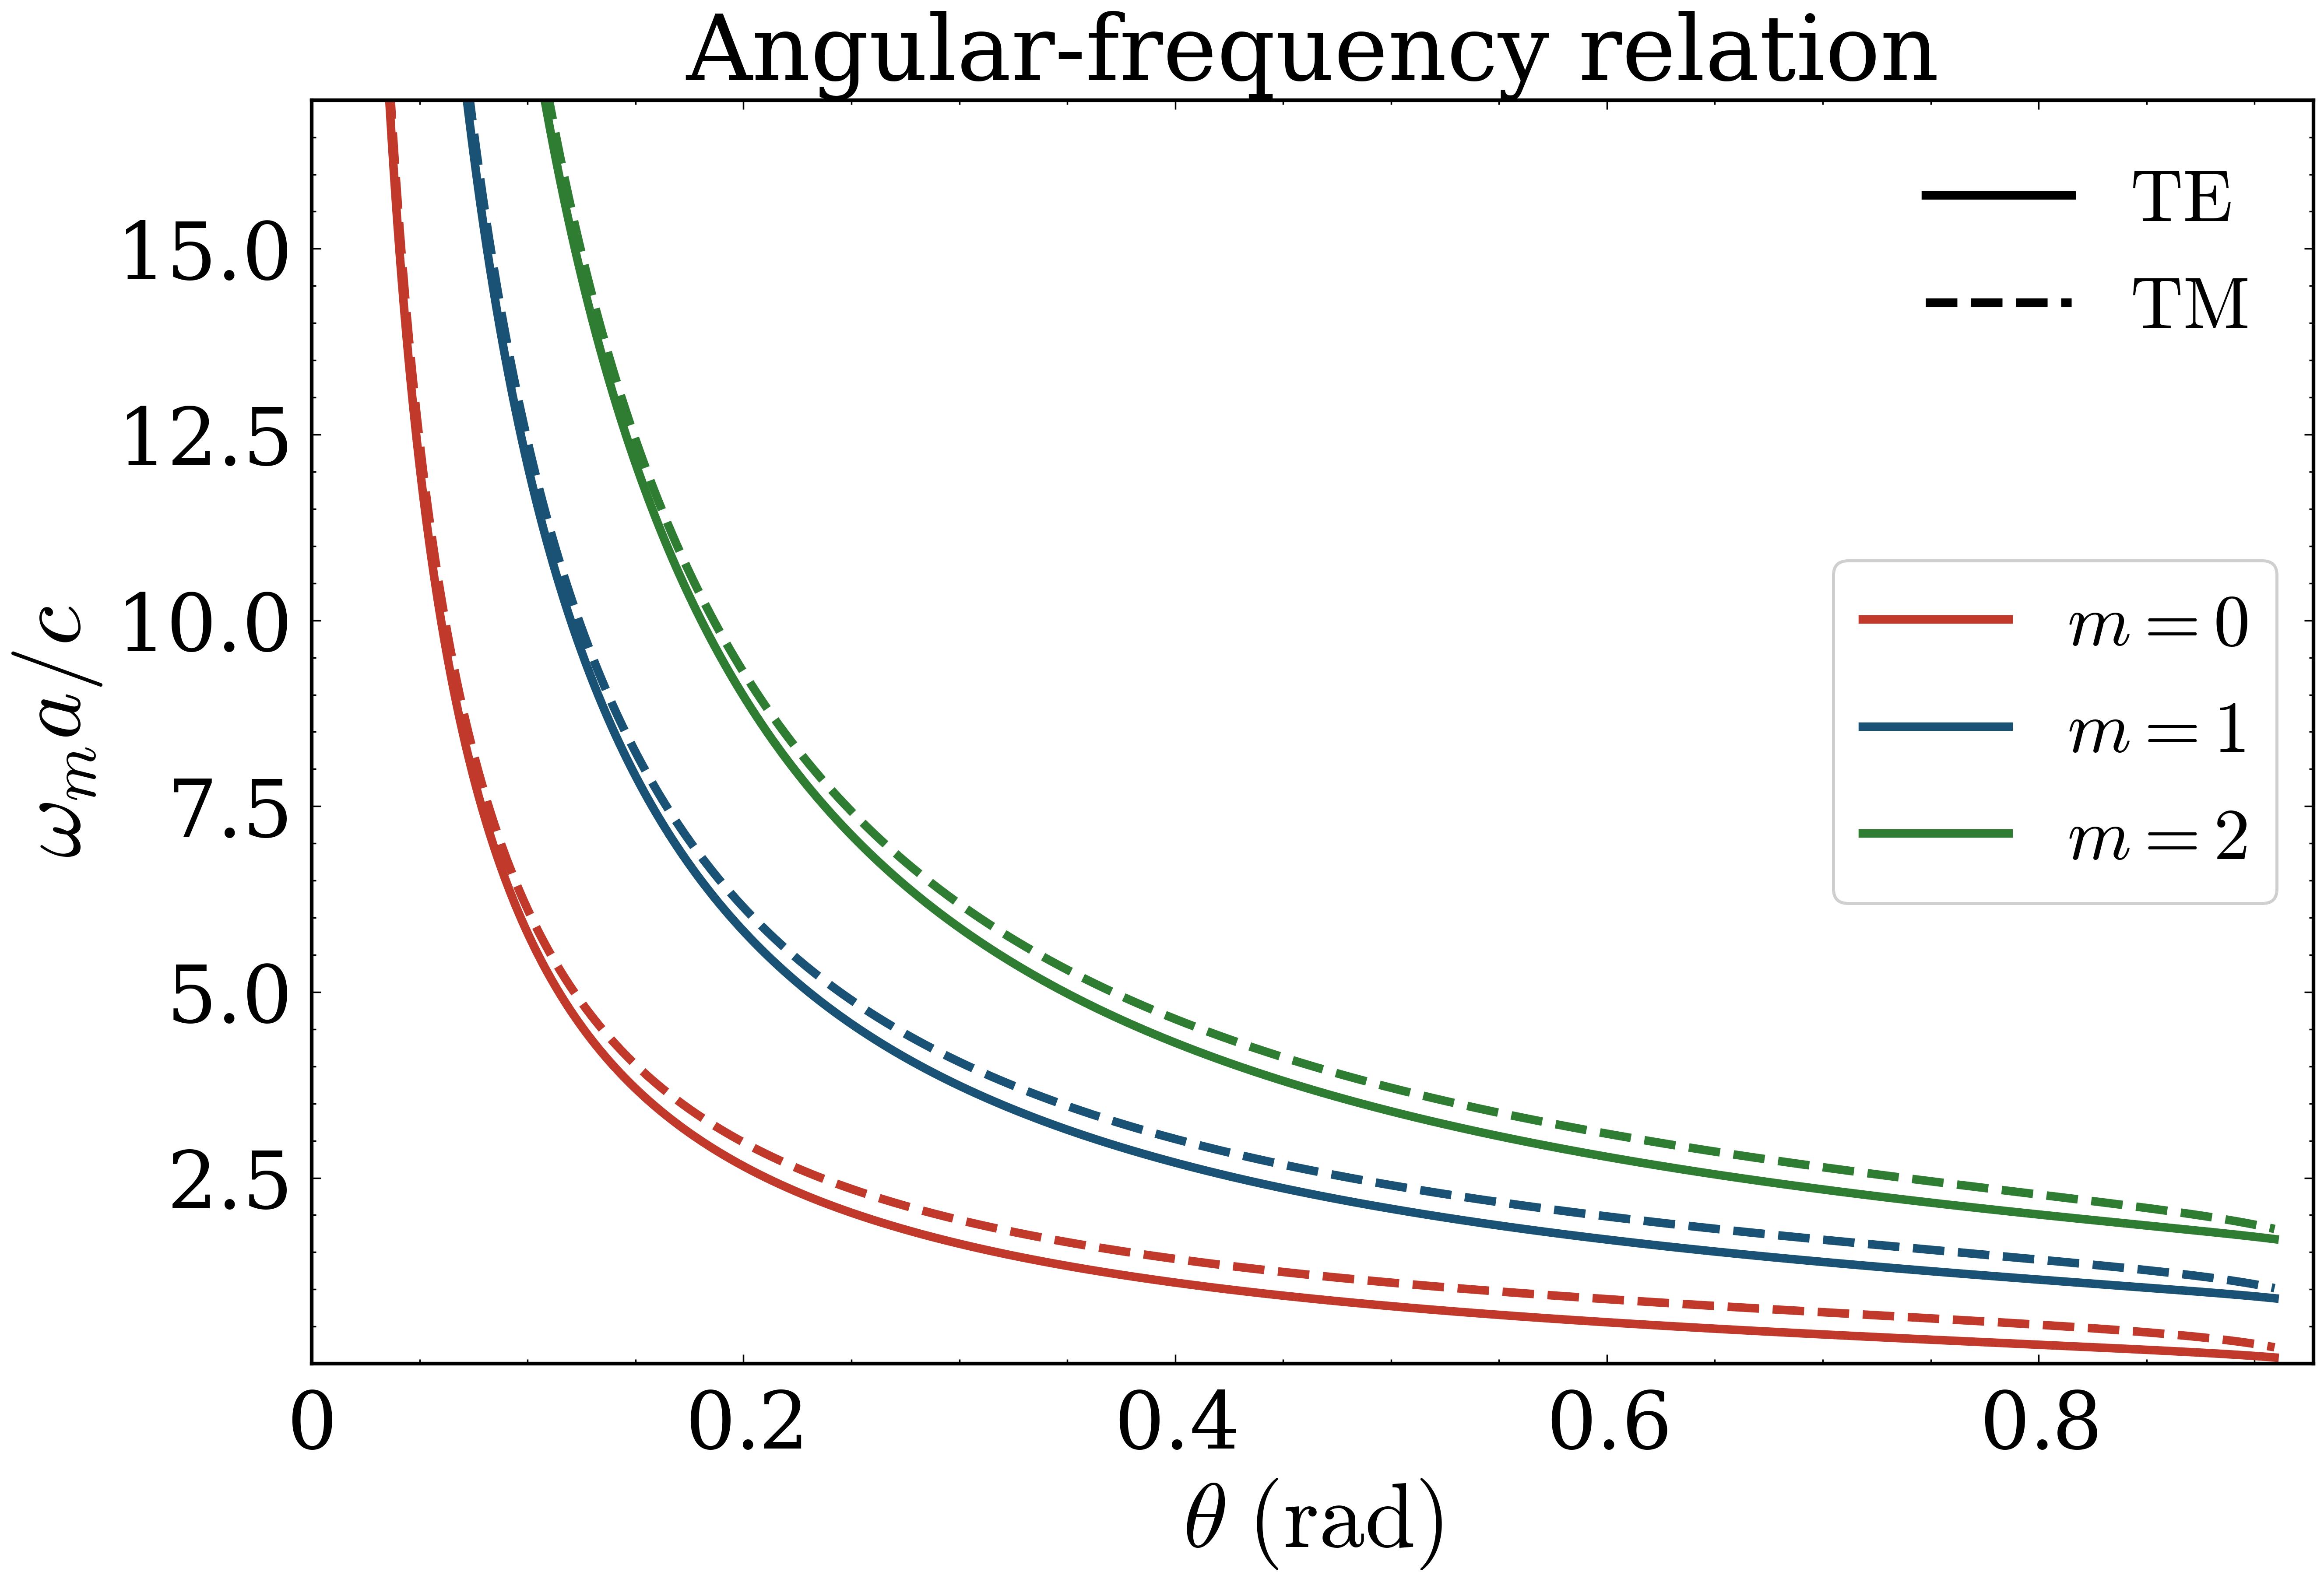
\includegraphics[width=\textwidth]{waveguide_fig/angular_frequency_relation.png}
		\caption{角频率关系图}
		\label{平面介质波导传播参量关系图(n_1=2.5,n_2=1.5)-角频率关系图}
	\end{subfigure}
	\hfill
	\begin{subfigure}[b]{0.33\textwidth}
		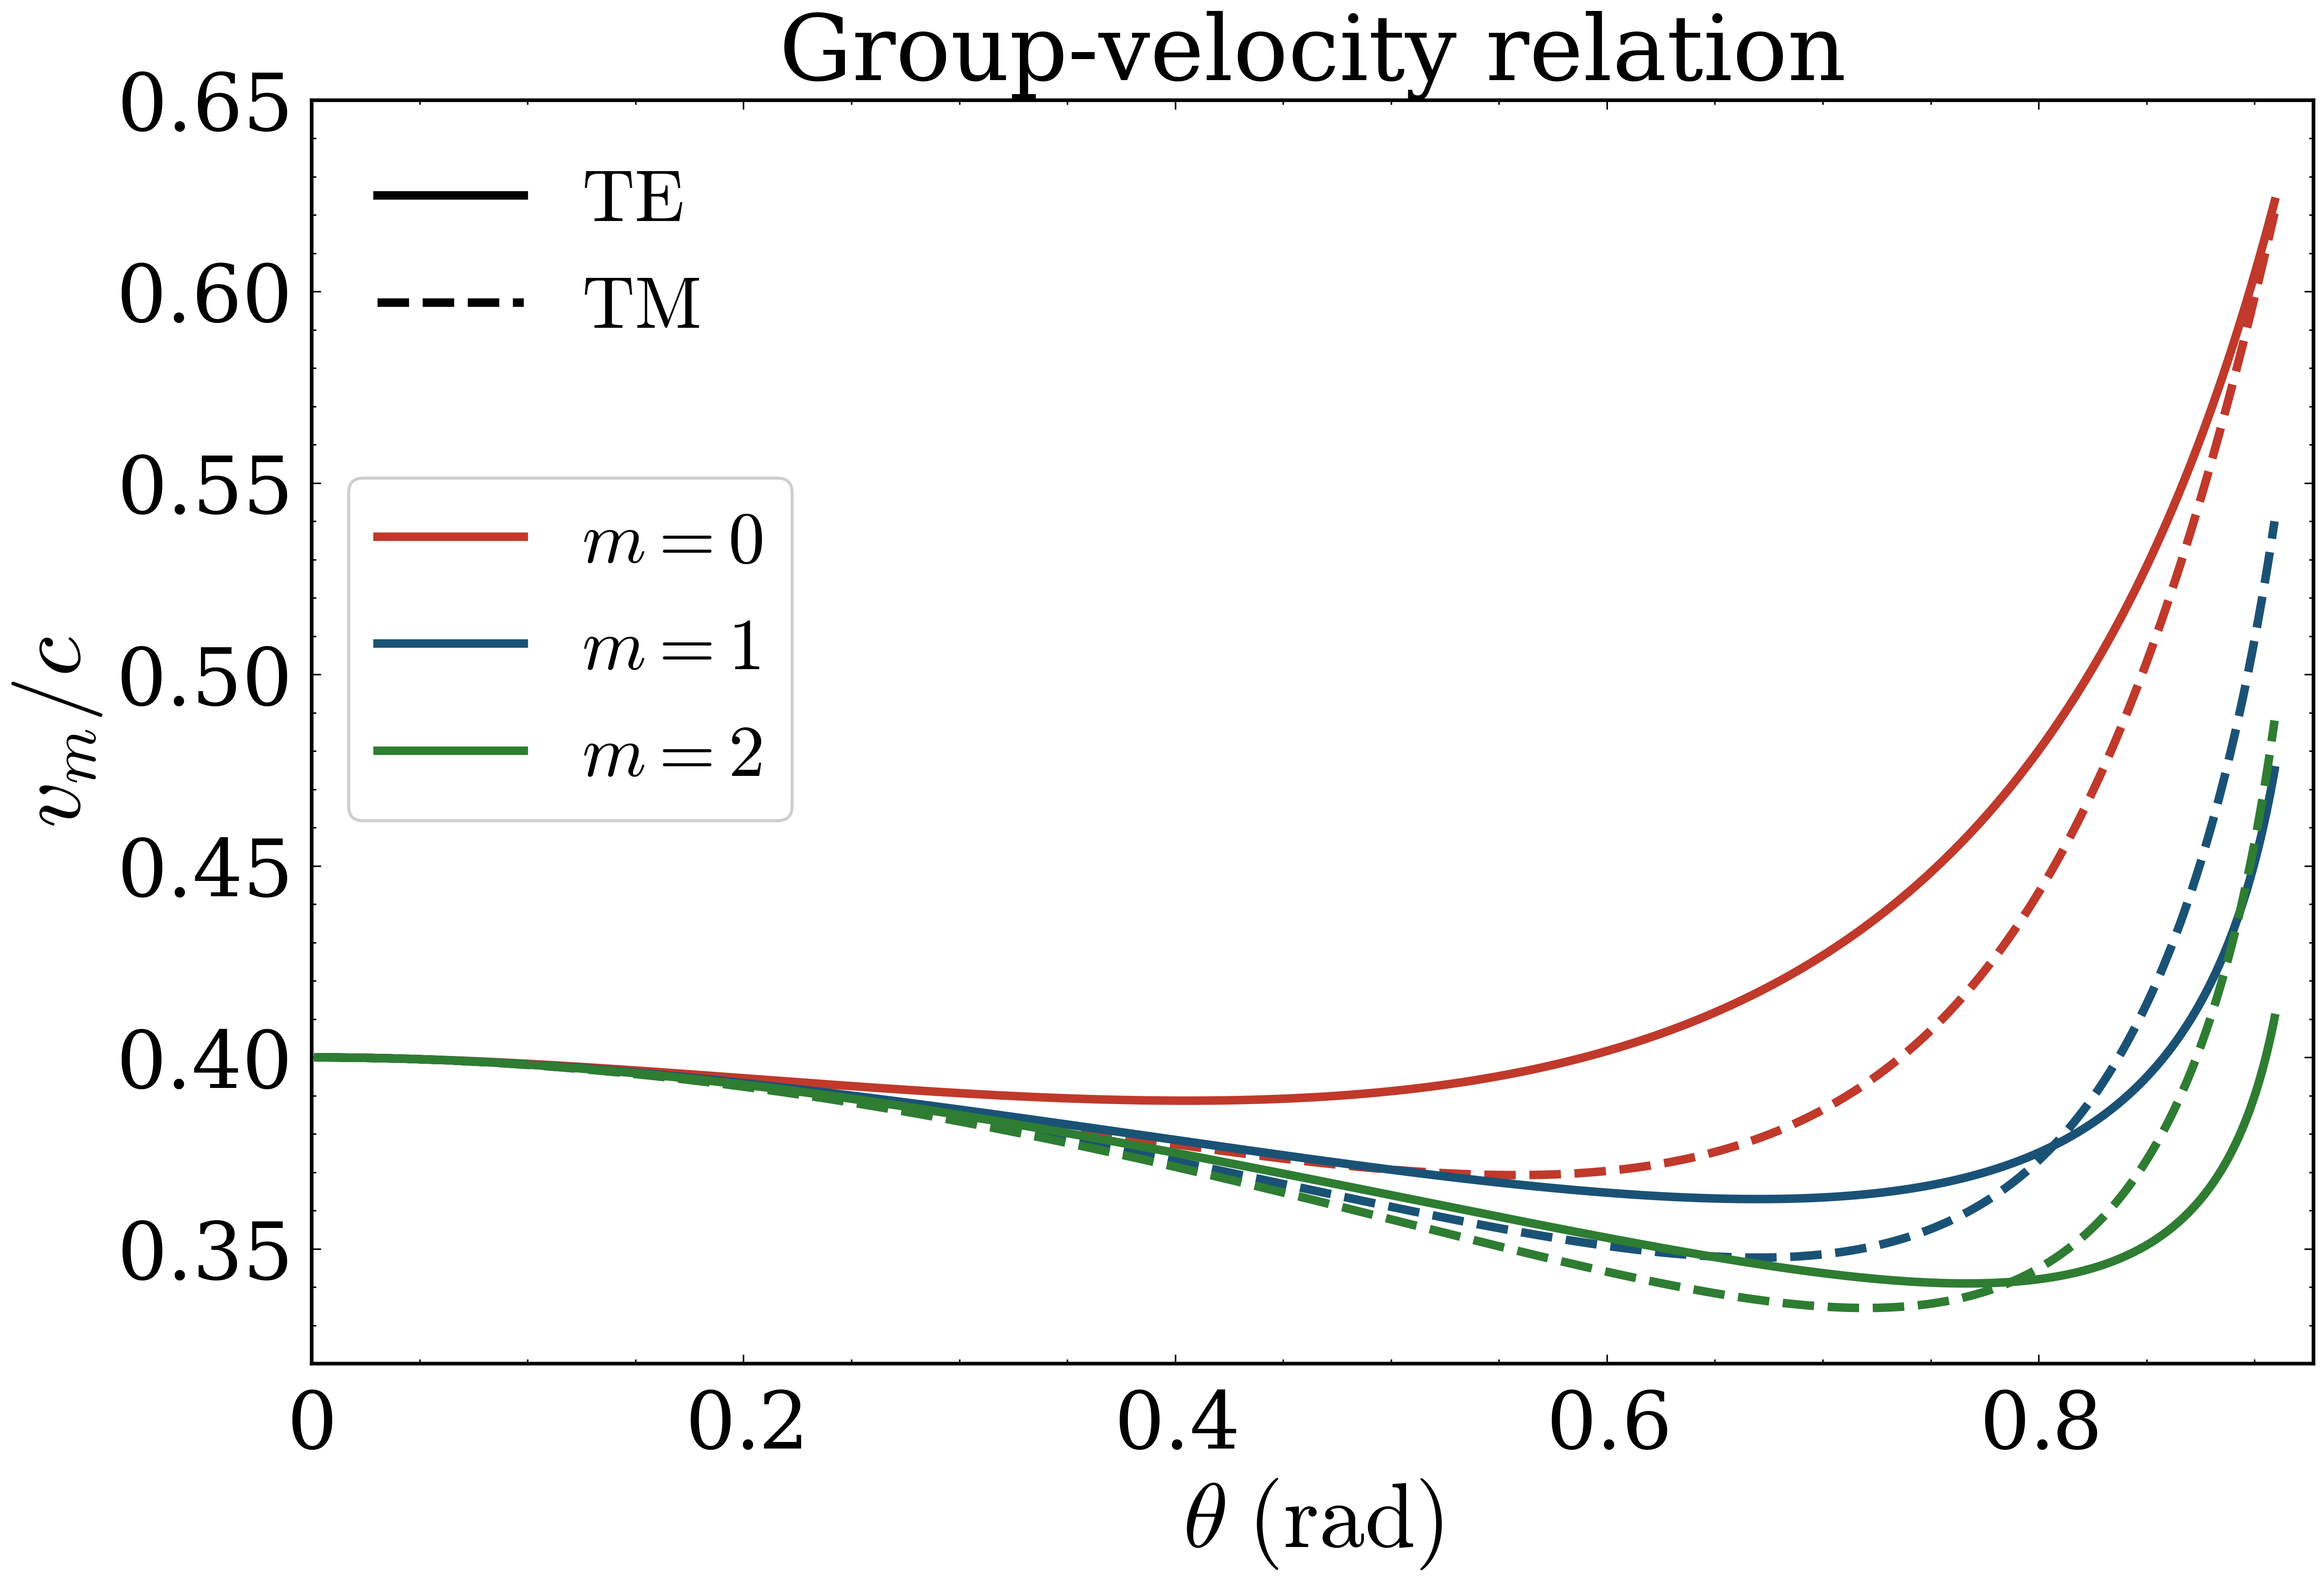
\includegraphics[width=\textwidth]{waveguide_fig/group_velocity_relation.png}
		\caption{群速度关系图}
		\label{平面介质波导传播参量关系图(n_1=2.5,n_2=1.5)-群速度关系图}
	\end{subfigure}
	\hfill
	\begin{subfigure}[b]{0.32\textwidth}
		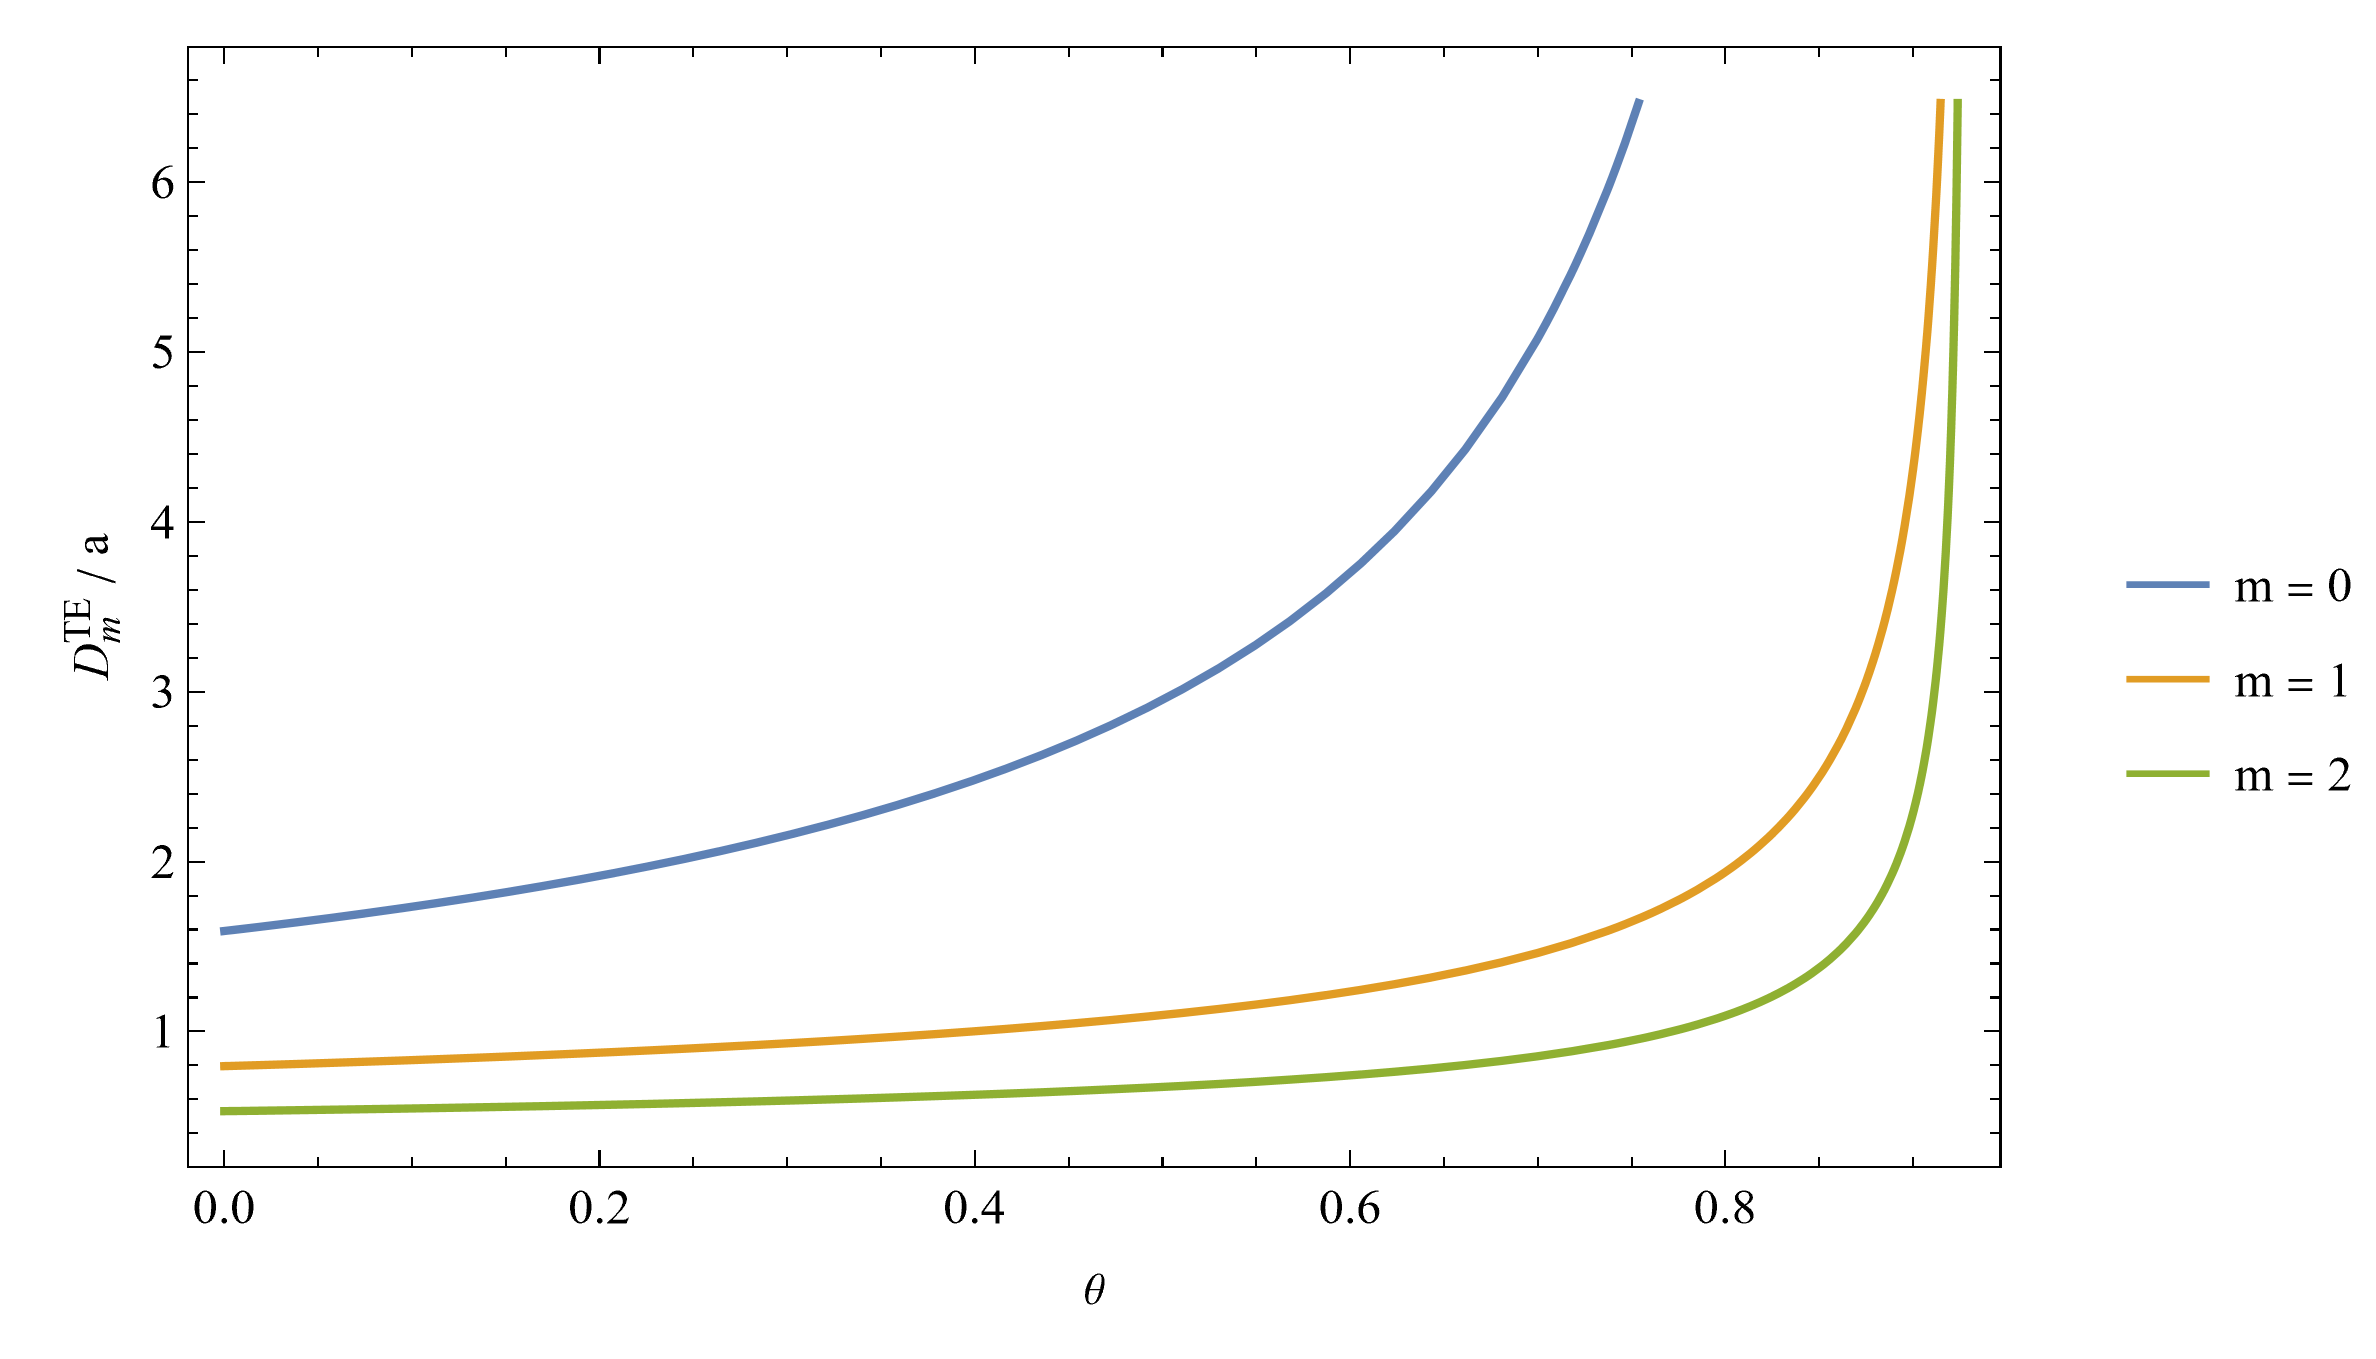
\includegraphics[width=\textwidth]{waveguide_fig/characteristic_displacement_relation.png}
		\caption{特征位移关系图}
		\label{平面介质波导传播参量关系图(n_1=2.5,n_2=1.5)-特征位移关系图}
	\end{subfigure}
\end{figure}

\subsubsection{柱状介质波导}

在折射率为 \( n_2 \) 的无限大空间中有半径为 \( a \)、折射率为 \( n_1 \) 的无限长柱形波导 (\( n_1 > n_2 \))

时谐因子记为 \( e^{-i\omega t} \)，下略去，设纵向电磁场具有形式
\( E_z = E (\rho) e^{im\phi + ikz} \)，\( H_z = H (\rho) e^{im\phi + ikz} \).

记 \( \gamma^2 = n_1^2 \omega^2/c^2 - k^2 \)，\( \beta^2 = k^2 - n_2^2 \omega^2/c^2 \)，由电磁场方程
\begin{equation*}
	\begin{cases}
		\left( \nabla_t^2 + \gamma^2 \right) E_z = 0, \quad \left( \nabla_t^2 + \gamma^2 \right) H_z = 0 & \rho < a, \\
		\left( \nabla_t^2 - \beta^2 \right) E_z = 0, \quad \left( \nabla_t^2 - \beta^2 \right) H_z = 0   & \rho > a.
	\end{cases}
\end{equation*}
并考虑到 \( E_z (\rho \to 0, \infty) \)、\( H_z (\rho \to 0, \infty) \) 有限，及 \( \rho = a \) 处 \( E_z \)、\( H_z \) 连续，解得
\begin{equation*}
	E_z = Z_0
	\begin{cases}
		A_e \dfrac{J_m(\gamma \rho)}{J_m(\gamma a)} e^{im\phi} & \rho < a, \\[8pt]
		A_e \dfrac{K_m(\beta \rho)}{K_m(\beta a)} e^{im\phi}   & \rho > a.
	\end{cases},\quad
	H_z =
	\begin{cases}
		A_h \dfrac{J_m(\gamma \rho)}{J_m(\gamma a)} e^{im\phi} & \rho < a, \\[8pt]
		A_h \dfrac{K_m(\beta \rho)}{K_m(\beta a)} e^{im\phi}   & \rho > a.
	\end{cases}
\end{equation*}
其中 \( m \in \mathbb{N} \)，为模式编号中的第一个序数.进而 (记 \( U = \gamma a \)，\( W = \beta a \)，\( \xi = \rho/a \))
\begin{equation*}
	\vb{E}_t|_{\rho < a} &= \dfrac{i}{\gamma^2} \left( k \nabla_t E_z - \omega\mu_0 \uv{z} \times \nabla_t H_z \right) \\
	&= \dfrac{Z_0 e^{im\phi}}{J_m(U)}  \left[ \left( \dfrac{ika A_e}{U} J_m'(U\xi) - \dfrac{m\omega a A_h}{U^2 \xi c} J_m(U\xi) \right) \uv{\rho} - \left( \dfrac{i\omega A_h}{Uc} J_m'(U\xi) + \dfrac{mka A_e}{U^2 \xi} J_m(U\xi) \right) \uv{\phi} \right].\\
	\vb{E}_t|_{\rho > a} &= -\dfrac{i}{\beta^2} \left( k \nabla_t E_z - \omega\mu_0 \uv{z} \times \nabla_t H_z \right) \\
	&= \dfrac{Z_0 e^{im\phi}}{K_m(W)} \left[ \left( -\dfrac{ika A_e}{W} K_m'(W\xi) + \dfrac{m\omega a A_h}{W^2 \xi c} K_m(W\xi) \right) \uv{\rho} + \left( \dfrac{i\omega a A_h}{Wc} K_m'(W\xi) + \dfrac{mka A_e}{W^2 \xi} K_m(W\xi) \right) \uv{\phi} \right].\\
	\vb{H}_t|_{\rho < a} &= \dfrac{i}{\gamma^2} \left( k \nabla_t H_z + \omega\varepsilon_0 n_1^2 \uv{z} \times \nabla_t E_z \right) \\
	&= \dfrac{e^{im\phi}}{J_m(U)} \left[ \left( \dfrac{ika A_h}{U} J_m'(U\xi) + \dfrac{m\omega a n_1^2 A_e}{U^2 \xi c} J_m(U\xi) \right) \uv{\rho} + \left( \dfrac{i\omega a n_1^2 A_e}{Uc} J_m'(U\xi) - \dfrac{mka A_h}{U^2 \xi} J_m(U\xi) \right) \uv{\phi} \right].\\
	\vb{H}_t|_{\rho > a} &= -\dfrac{i}{\beta^2} \left( k \nabla_t H_z + \omega\mu_0 n_2^2 \uv{z} \times \nabla_t E_z \right) \\
	&= \dfrac{e^{im\phi}}{K_m(W)} \left[ \left( -\dfrac{ika A_h}{W} K_m'(W\xi) + \dfrac{m\omega a n_2^2 A_e}{W^2 \xi c} K_m(W\xi) \right) \uv{\rho} + \left( -\dfrac{i\omega a n_2^2 A_e}{Wc} K_m'(W\xi) + \dfrac{mka A_h}{W^2 \xi} K_m(W\xi) \right) \uv{\phi} \right].
\end{equation*}
再根据边界条件
\begin{equation*}
	n_1^2 \vb{E}_t \cdot \uv{\rho}|_{\rho = a^-} = n_2^2 \vb{E}_t \cdot \uv{\rho}|_{\rho = a^+},\,\,E_z|_{\rho = a^-} = E_z|_{\rho = a^+} ,\,\,\vb{E}_t \cdot \uv{\phi}|_{\rho = a^-} = \vb{E}_t \cdot \uv{\phi}|_{\rho = a^+}
\end{equation*}\begin{equation*}
	H_z|_{\rho = a^-} = H_z|_{\rho = a^+},\,\,\vb{H}_t \cdot \uv{\phi}|_{\rho = a^-} = \vb{H}_t \cdot \uv{\phi}|_{\rho = a^+}.
\end{equation*}
解得
\begin{equation*}
	\dfrac{A_h}{A_e} = \dfrac{i\omega}{mkc} \cdot \dfrac{n_1^2 f_m(U) + n_2^2 g_m(W)}{1/U^2 + 1/W^2} = \dfrac{imkc}{\omega} \cdot \dfrac{1/U^2 + 1/W^2}{f_m(U)+g_m(W)}.
\end{equation*}
其中 \( f_m(x) = \dfrac{J_m'(x)}{x J_m(x)} \)，\( g_m(x) = \dfrac{K_m'(x)}{x K_m(x)} \).故本征方程为
\begin{equation*}
	\mathcal{F}_m(U, W) = \left( n_1^2 f_m(U) + n_2^2 g_m(W) \right) \left( f_m(U) + g_m(W) \right) - m^2 \left( 1/U^2 + 1/W^2 \right) \left( n_1^2/U^2 + n_2^2/W^2 \right) = 0.
\end{equation*}
式中用到
\begin{equation*}
	ka = \sqrt{\dfrac{n_2^2 U^2 + n_1^2 W^2}{n_1^2 - n_2^2}}, \quad \dfrac{\omega a}{c} = \sqrt{\dfrac{U^2 + W^2}{n_1^2 - n_2^2}}.
\end{equation*}

接着考虑能量传输特征
内层 (core)、外层 (clad) 沿波导延伸方向的传输功率为
\begin{equation*}
	\small
	\begin{split}
		P_{\text{core}} & = \frac{1}{2} \pi (1 + \delta_{m0}) \int_0^a \Re\left[ \vec{\mathbf{E}} \times \vec{\mathbf{H}}^* \cdot \hat{\mathbf{z}} \right] \rho \, \d \rho                          \\
		                & = -\frac{(1 + \delta_{m0}) \pi a^2 |A_e|^2 \omega k a^2}{4 Z_0 c (f_m(U) + g_m(W))} \cdot \frac{\partial \mathcal{F}_m(U, W)}{\partial U} \cdot \frac{1}{U}               \\
		                & = -\frac{(1 + \delta_{m0}) \pi a^2 |A_e|^2 \omega k a^2}{4 Z_0 U c (f_m(U) + g_m(W))} \Bigg[ \left( n_1^2 (f_m(U) + g_m(W)) + n_1^2 f_m(U) + n_2^2 g_m(W) \right) f_m'(U) \\
		                & \quad + 2 m^2 \cdot \frac{(n_1^2 + n_2^2) U^2 + 2 n_1^2 W^2}{U^5 W^2} \Bigg].                                                                                             \\
		\\
		P_{\text{clad}} & = \frac{1}{2} \pi (1 + \delta_{m0}) \int_a^\infty \Re\left[ \vec{\mathbf{E}} \times \vec{\mathbf{H}}^* \cdot \hat{\mathbf{z}} \right] \rho \, \d \rho                     \\
		                & = \frac{(1 + \delta_{m0}) \pi a^2 |A_e|^2 \omega k a^2}{4 Z_0 c (f_m(U) + g_m(W))} \cdot \frac{\partial \mathcal{F}_m(U, W)}{\partial W} \cdot \frac{1}{W}                \\
		                & = \frac{(1 + \delta_{m0}) \pi a^2 |A_e|^2 \omega k a^2}{4 Z_0 W c (f_m(U) + g_m(W))} \Bigg[ \left( n_2^2 (f_m(U) + g_m(W)) + n_1^2 f_m(U) + n_2^2 g_m(W) \right)g_m'(W)   \\
		                & \quad + 2 m^2 \cdot \frac{(n_1^2 + n_2^2) W^2 + 2 n_2^2 U^2}{W^5 U^2} \Bigg].
	\end{split}
	\normalsize
\end{equation*}
式中，\(\pi (1 + \delta_{m0})\) 因子来源于对 \(\phi\) 的积分（\(\vb{E} \times \vb{H}^*\) 过程消除了角向依赖，需要在传输功率部分将其补齐）.

对本征值方程微分，得群速度为
\begin{equation*}
	\dfrac{U \d U}{W \d W} = \dfrac{P_{\text{clad}}}{P_{\text{core}}}, \quad v_g = \dfrac{\d \omega}{\d k} = \dfrac{c^2 k}{\omega} \cdot \dfrac{U \d U + W \d W}{n_2^2 U \d U + n_1^2 W \d W} = \dfrac{c^2 k}{\omega} \cdot \dfrac{P_{\text{clad}} + P_{\text{core}}}{n_2^2 P_{\text{clad}} + n_1^2 P_{\text{core}}}.
\end{equation*}

以下具体考察本征值方程给出的各种模式.易知，本征值分为两个特征支
\begin{equation*}
	f_m(U) = -\dfrac{1}{2} \left( 1 + \dfrac{n_2^2}{n_1^2} \right) g_m(W) \pm \sqrt{\dfrac{1}{4} \left( 1 - \dfrac{n_2^2}{n_1^2} \right)^2 g_m^2(W) + m^2 \left( \dfrac{1}{U^2} + \dfrac{1}{W^2} \right) \left( \dfrac{1}{U^2} + \dfrac{n_2^2}{n_1^2 W^2} \right)}.
\end{equation*}
规定上符号对应 \(\mathrm{EH}_{mn}\) 或 \(\mathrm{TE}_{0n}\) 模式，下符号对应 \(\mathrm{HE}_{mn}\) 或 \(\mathrm{TM}_{0n}\) 模式.特别地，\(n_1 = 2.5,\,n_2 = 1.5\) 情形如图\ref{圆柱波导传输模式图}，图中\(V = \sqrt{U^2 + W^2}\)，\(\Delta = (n_1^2 - n_2^2)/(2 n_1^2)\).

对于 \(m \geq 2\)，\(U-W\) 等高线族由无穷多条互不相交的、与 \(U\) 轴相交、不过原点的曲线组成，根据曲线的数学特征，等高线族可分为两组特征曲线，分别记为 \(\mathrm{HE}_{mn}\) 和 \(\mathrm{EH}_{mn}\)（\(n \in \mathbb{Z}^+\)）模式.

对于 \(m = 1\)，则等高线族中存在一条曲线经过原点（记为 \(\mathrm{HE}_{11}\) 模式），其他曲线除了两两在 \(U\) 轴相交外，在 \(\beta > 0\) 的区域互不相交，同样，根据数学特征，曲线可分为 \(\mathrm{HE}_{mn}\) 和 \(\mathrm{EH}_{mn}\) 模式.

对于 \(m = 0\)，则所有曲线除了两两在 \(U\) 轴相交外，在 \(W > 0\) 的区域互不相交、且不过原点，同样，根据数学特征，曲线可分为 \(\mathrm{TM}_{0n}\)（对应 \(A_h = 0\)，\(A_e \neq 0\)）和 \(\mathrm{TE}_{0n}\)（对应 \(A_e = 0\)，\(A_h \neq 0\)）模式.

事实上，\(m \geq 1\) 时，纵向电场或磁场均不为零（平庸解除外），因此 \(\mathrm{HE},\,\mathrm{EH}\)属于混合模式.而 \(m = 0\) 时，纵向电场或磁场必有其一为零，因此可以区分 \(\mathrm{TM},\,\mathrm{TE}\) 模式.

再观察芯层传输功率比率与频率关系图\ref{圆柱波导传输效率图} ，图中 \(\eta =P_{\text{core}}/(P_{\text{core}} + P_{\text{clad}})\).由图可见，\(W = 0\) 时 \(\eta\) 最小，对应截止状态, 对 \(\mathrm{TE}_{0n},\,\mathrm{TM}_{0n},\,\mathrm{HE}_{1n},\,\mathrm{HE}_{2n}\) 模式 \(\eta\) 可达到零，即能量全部在包层中传播，对其他模式 \(\eta\) 最小值大于零，即能量总有一部分会在芯层中传播.\(W \gg 1\) 时 \(\eta\) 趋于 1，即能量全部在芯层中传播，对应远离截止的状态.

\begin{figure}[htbp]
	\centering
	\begin{minipage}{0.49\textwidth}
		\centering
		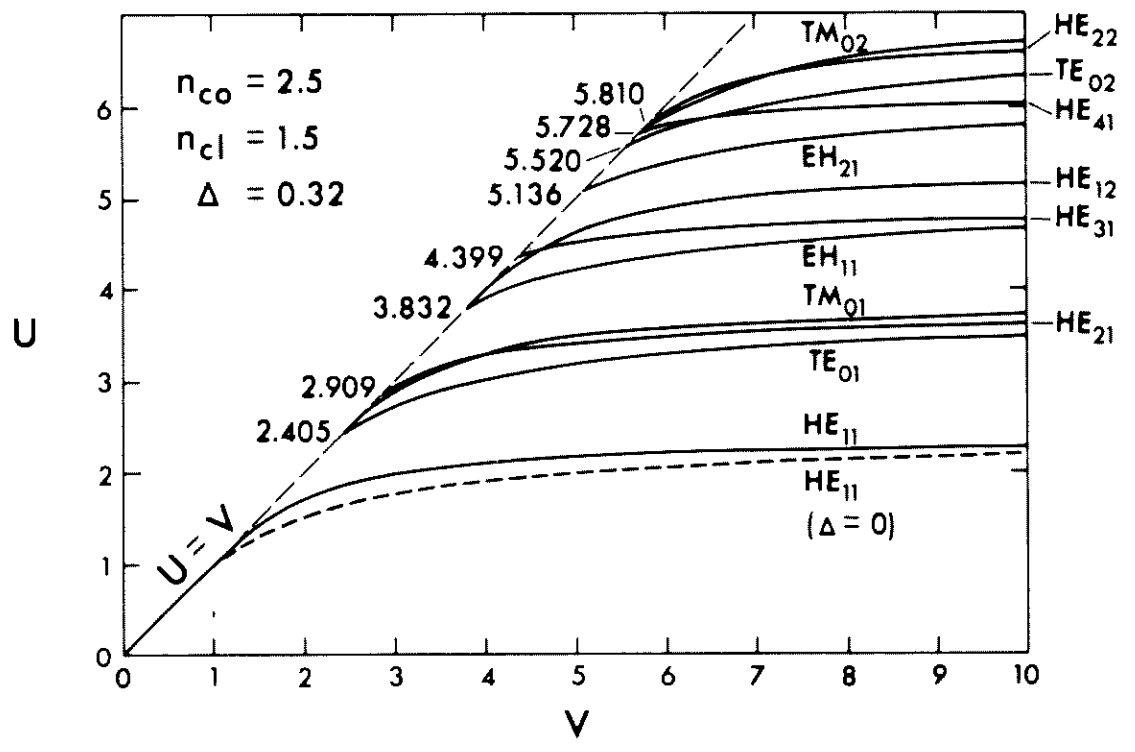
\includegraphics[width=\textwidth]{waveguide_fig/propagation_mode_schematic_diagram_n_1_2_5_n_2_1_5.png}
		\caption{传播模式示意图(\(n_1 = 2.5,\,n_2=1.5\))}
		\label{传播模式示意图(n_1=2.5,n_2=1.5)}
		\label{圆柱波导传输模式图}
	\end{minipage}
	\hfill
	\begin{minipage}{0.49\textwidth}
		\centering
		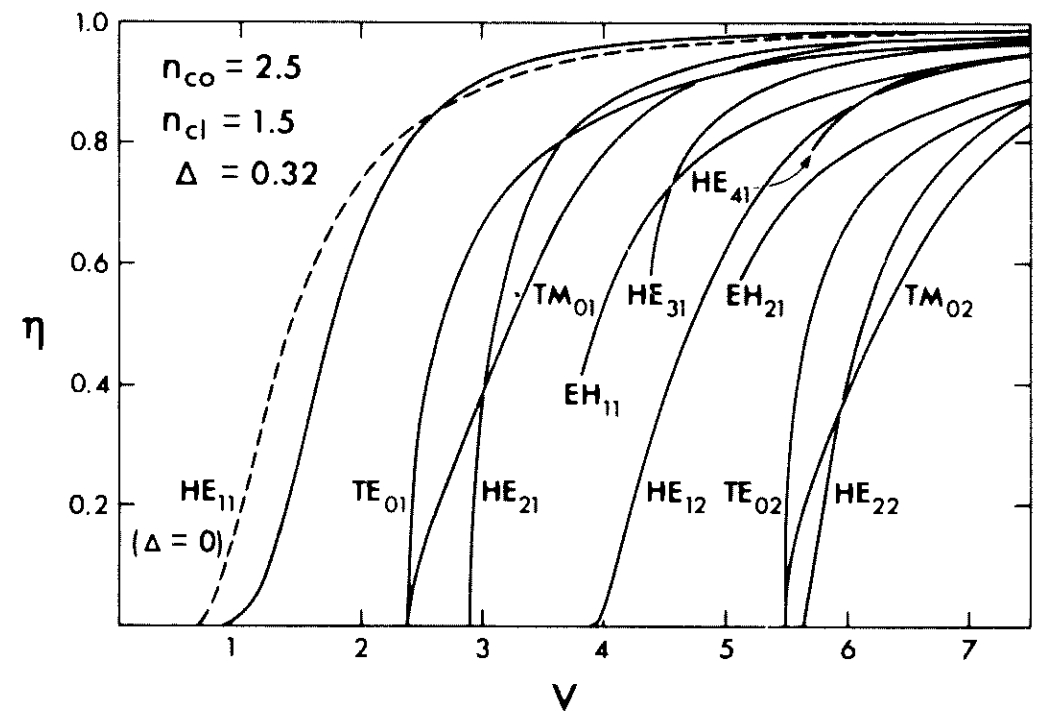
\includegraphics[width=\textwidth]{waveguide_fig/transmission_efficiency_relation_plot_n_1_2_5_n_2_1_5.png}
		\caption{传输效率关系图(\(n_1=2.5,\,n_2=1.5\))}
		\label{传输效率关系图(n_1=2.5,n_2=1.5)}
		\label{圆柱波导传输效率图}
	\end{minipage}
\end{figure}

截止处 （\(W \to 0\)） 及远离截止处 （\(W \gg 1\)） 各物理量的极限行为如下
\begin{equation*}
	&W \approx 2 \exp\left( -\gamma_E - \dfrac{n_1^2 + n_2^2}{2 n_1^2 U^2} \right) \bigg|_{U \ll 1} \to 0, \quad \mathrm{HE}_{11}\\
	&U|_{W=0} =
	\begin{cases}
		\mu_{0n}    & \mathrm{TE}_{0n},\, \mathrm{TM}_{0n} \, , \\
		\mu_{mn}    & \mathrm{EH}_{mn} \, ,                     \\
		\kappa_{mn} & \mathrm{HE}_{mn} \, ,                     \\
		0           & \mathrm{HE}_{11} \, .
	\end{cases},\quad
	U|_{W \gg 1} \approx
	\begin{cases}
		\mu_{1n} \left( 1 - \dfrac{1}{W} \right)                        & \mathrm{TE}_{0n} \, , \\[8pt]
		\mu_{1n} \left( 1 - \dfrac{n_2^2}{n_1^2 W} \right)              & \mathrm{TM}_{0n} \, , \\[8pt]
		\mu_{m+1,n} \left( 1 - \dfrac{n_1^2 + n_2^2}{2 n_1^2 W} \right) & \mathrm{EH}_{mn} \, , \\[8pt]
		\mu_{m-1,n} \left( 1 - \dfrac{n_1^2 + n_2^2}{2 n_1^2 W} \right) & \mathrm{HE}_{mn} \, .
	\end{cases}\\
	&\left. \dfrac{P_{\text{core}}}{P_{\text{clad}}} \right|_{W \to 0} =
	\begin{cases}
		\dfrac{m(n_1^2 + n_2^2)}{2 n_1^2}                                                                                                                                                                                                                                                                                                                & \mathrm{EH}_{mn} \, , \\
		\dfrac{m\left(m-1\right)^2\left(m-2\right) \kappa_{mn} \left(n_1^2 + n_2^2\right)^3 \left( 2m\kappa_{mn}^{-3} - f_m'\left(\kappa_{mn}\right) \right)}{-m\left(m-1\right)\left(m-2\right)\left(n_1^2 + n_2^2\right)\left(n_1^2 - n_2^2\right)^2 + n_2^2 \left( \left(m-1\right)n_1^4 + 2n_1^2n_2^2 + \left(m-1\right)n_2^4 \right) \kappa_{mn}^2} & \mathrm{HE}_{mn} \, .
	\end{cases}
\end{equation*}
这进一步说明，\(\mathrm{TE}_{0n}\) 及 \(\mathrm{TM}_{0n}\) 模式的\(U\)位于 \(\mu_{0n}\) 和 \(\mu_{1n}\) 之间，\(\mathrm{EH}_{mn}\) 模式的\(U\)位于 \(\mu_{mn}\) 和 \(\mu_{m+1,n}\) 之间，\(\mathrm{HE}_{mn}\) 模式的\(U\)位于 \(\kappa_{mn}\) 和 \(\mu_{m-1,n}\) 之间.

特别地，对于弱传播波导（\(n_1\approx n_2\)），本征值方程退化为
\begin{equation*}
	\dfrac{J_j(U)}{U J_{j-1}(U)} = -\dfrac{K_j(W)}{W K_{j-1}(W)}, \quad j =
	\begin{cases}
		1   & \mathrm{TE}_{0n}, \, \mathrm{TM}_{0n} , \\
		m+1 & \mathrm{EH}_{mn} ,                      \\
		m-1 & \mathrm{HE}_{mn} .
	\end{cases}
\end{equation*}
此时，各模式出现简并，不妨定义新的 \(\mathrm{LP}_{mn}\) (linearly polarized, \(m \in \mathbb{N}\)，\(n \in \mathbb{Z}^+\)) 模式，对应
\begin{equation*}
	\dfrac{J_m(U)}{U J_{m-1}(U)} = -\dfrac{K_m(W)}{W K_{m-1}(W)}, \quad \mathrm{LP}_{mn} \, .
\end{equation*}
可见，原先的各模式将并入LP模式，对应
\begin{equation*}
	\mathrm{HE}_{1n} \to \mathrm{LP}_{0n},\quad (\mathrm{TE}_{0n}, \mathrm{TM}_{0n}, \mathrm{HE}_{2n}) \to \mathrm{LP}_{1n},\quad (\mathrm{HE}_{m+1,n}, \mathrm{EH}_{m-1,n}) \to \mathrm{LP}_{mn}\ (m \geq 2).
\end{equation*}

另外，不难求出\(\mathrm{TE}_{0n},\,\mathrm{TM}_{0n}\)模式的严格解.对于\(\mathrm{TE}_{0n}\) 模式
\begin{equation*}
	&-(f_0(U) + g_0(W)) = \dfrac{J_1(U)}{U J_0(U)} + \dfrac{K_1(W)}{W K_0(W)} = 0, \quad A_e = 0, \quad A_h \neq 0.\\
	&\vb{E}_t = \dfrac{i \omega a Z_0 A_h}{c} \uv{\phi}
	\begin{cases}
		\dfrac{J_1(U\xi)}{U J_0(U)}  & \xi < 1, \\[8pt]
		-\dfrac{K_1(W\xi)}{W K_0(W)} & \xi > 1.
	\end{cases}
	\quad
	\vb{H}_t = i k a A_h \uv{\rho}
	\begin{cases}
		-\dfrac{J_1(U\xi)}{U J_0(U)} & \xi < 1, \\[8pt]
		\dfrac{K_1(W\xi)}{W K_0(W)}  & \xi > 1.
	\end{cases}
	\quad
	H_z = A_h
	\begin{cases}
		\dfrac{J_0(U\xi)}{U J_0(U)} & \xi < 1, \\[8pt]
		\dfrac{K_0(W\xi)}{W K_0(W)} & \xi > 1.
	\end{cases}\\
	&P_{\text{core}} = \dfrac{1}{2} \int_0^a \Re\left[ \vb{E} \times \vb{H}^* \cdot \uv{z} \right] 2\pi \rho \, \d \rho = \dfrac{\pi a^2 Z_0 |A_h|^2 \omega k a^2}{2 U^2 c} \left( \dfrac{J_1(U)}{J_0(U)} \right)^2 \left( 1 - \dfrac{J_0(U) J_2(U)}{|J_1(U)|^2} \right).\\
	&P_{\text{clad}} = \dfrac{1}{2} \int_a^\infty \Re\left[ \vb{E} \times \vb{H}^* \cdot \uv{z} \right] 2\pi \rho \, \d \rho = -\dfrac{\pi a^2 Z_0 |A_h|^2 \omega k a^2}{2 W^2 c} \left( \dfrac{K_1(W)}{K_0(W)} \right)^2 \left( 1 - \dfrac{K_0(W) K_2(W)}{|K_1(W)|^2} \right).
\end{equation*}
对于\(\mathrm{TM}_{0n}\) 模式
\begin{equation*}
	&-(n_1^2 f_0(U) + n_2^2 g_0(W)) = \dfrac{n_1^2 J_1(U)}{U J_0(U)} + \dfrac{n_2^2 K_1(W)}{W K_0(W)} = 0, \quad A_h = 0, \quad A_e \neq 0.\\
	&\vb{E}_t = i k a Z_0 A_e \uv{\rho}
	\begin{cases}
		-\dfrac{J_1(U\xi)}{U J_0(U)} & \xi < 1, \\[8pt]
		\dfrac{K_1(W\xi)}{W K_0(W)}  & \xi > 1.
	\end{cases}
	\quad
	E_z = Z_0 A_e
	\begin{cases}
		\dfrac{J_0(U\xi)}{U J_0(U)} & \xi < 1, \\[8pt]
		\dfrac{K_0(W\xi)}{W K_0(W)} & \xi > 1.
	\end{cases}
	\quad
	\vb{H}_t = \dfrac{i \omega a A_e}{c} \uv{\rho}
	\begin{cases}
		-\dfrac{n_1^2 J_1(U\xi)}{U J_0(U)} & \xi < 1, \\[8pt]
		\dfrac{n_2^2 K_1(W\xi)}{W K_0(W)}  & \xi > 1.
	\end{cases}\\
	&P_{\text{core}} = \dfrac{1}{2} \int_0^a \Re\left[ \vb{E} \times \vb{H}^* \cdot \uv{z} \right] 2\pi \rho \, \d \rho = \dfrac{\pi a^2 Z_0 |A_e|^2 n_1^2 \omega k a^2}{2 c} \left( \dfrac{J_1(U)}{U J_0(U)} \right)^2 \left( 1 - \dfrac{J_0(U) J_2(U)}{|J_1(U)|^2} \right).\\
	&P_{\text{clad}} = \dfrac{1}{2} \int_a^\infty \Re\left[ \vb{E} \times \vb{H}^* \cdot \uv{z} \right] 2\pi \rho \, \d \rho = -\dfrac{\pi a^2 Z_0 |A_e|^2 n_2^2 \omega k a^2}{2 c} \left( \dfrac{K_1(W)}{W K_0(W)} \right)^2 \left( 1 - \dfrac{K_0(W) K_2(W)}{|K_1(W)|^2} \right).
\end{equation*}

以上计算中，\(\mu_{mn}\) 是 \(J_m(x) = 0\) 的第\(n\)个正实根，\(\gamma_E \approx 0.5772\) 为欧拉伽马常数，\(\kappa_{mn}\) 是以下方程的第\(n\)个非负实根 （\(m = 1\) 时退化为 \(\kappa_{1n} = \mu_{1,n-1}\)，\(\kappa_{11} = 0\)）.
\begin{equation*}
	\dfrac{x J_{m-2}(x)}{J_{m-1}(x)} + (m-1) \dfrac{n_1^2 - n_2^2}{n_2^2} = 0.
\end{equation*}
并用到数学公式
\begin{equation*}
	&f_m(x) =
	\begin{cases}
		-\dfrac{1}{2} - \dfrac{x^2}{16} + O(x^4)    & m=0,\ x \ll 1,      \\[8pt]
		\dfrac{m}{x^2} - \dfrac{1}{2(m+1)} + O(x^2) & m \geq 1,\ x \gg 1.
	\end{cases}
	\quad
	g_m(x) =
	\begin{cases}
		\dfrac{1}{x^2 \left( \gamma_E + \ln \dfrac{x}{2} \right)^{-1}} + O(x^0) & m=0,\ x \ll 1,      \\[8pt]
		-\dfrac{1}{x^2} + \gamma_E + \ln \dfrac{x}{2} + O(x)                    & m=1,\ x \ll 1,      \\[8pt]
		-\dfrac{m}{x^2} - \dfrac{1}{2(m-1)} + O(x^2)                            & m \geq 2,\ x \ll 1, \\[8pt]
		-\dfrac{1}{x} + O(x^{-2})                                               & x \to \infty.
	\end{cases}\\[8pt]
	&\left. f_m(x) \right|_{x \to \mu_{mn}} = \dfrac{1}{\mu_{mn} (x - \mu_{mn})},
	\quad
	\dfrac{\d g_m(x)}{\d x} =
	\begin{cases}
		-\dfrac{2\gamma_E + 1 + 2\ln \dfrac{x}{2}}{\left( \gamma_E + \ln \dfrac{x}{2} \right)^2 x^3} + O(x^{-1}) & m=0,      \\[8pt]
		\dfrac{2}{x^3} + \dfrac{1}{x} + O(x)                                                                     & m=1,      \\[8pt]
		\dfrac{4}{x^3} - \dfrac{1}{4} \left( 2\gamma_E + 1 + 2\ln \dfrac{x}{2} \right) x + O(x^3)                & m=2,      \\[8pt]
		\dfrac{2m}{x^3} + \dfrac{x}{4(m-1)^2(m-2)} + O(x^3)                                                      & m \geq 3.
	\end{cases}
\end{equation*}

模型中涉及的部分数值参量如下.
\begin{table}[htbp]
	\renewcommand{\arraystretch}{1.2}
	\begin{minipage}{0.48\textwidth}
		\centering
		\begin{tabular}{|c|c|c|c|c|}
			\toprule
			\diagbox[width=2cm,height=0.8cm]{\(m\)}{\(n\)} & \makecell{1} & \makecell{2} & \makecell{3} & \makecell{4} \\
			\midrule
			0                                              & 2.4048       & 5.5201       & 8.6537       & 11.7915      \\
			1                                              & 3.8317       & 7.0156       & 10.1735      & 13.3237      \\
			2                                              & 5.1356       & 8.4172       & 11.6198      & 14.7960      \\
			3                                              & 6.3802       & 9.7610       & 13.0152      & 16.2235      \\
			\bottomrule
		\end{tabular}
		\caption{\(\mu_{mn}\)数值表}
		\label{mu_mn数值表}
	\end{minipage}
	\hfill
	\begin{minipage}{0.48\textwidth}
		\centering
		\begin{tabular}{|c|c|c|c|c|}
			\toprule
			\diagbox[width=2cm,height=0.8cm]{\(m\)}{\(n\)} & \makecell{1} & \makecell{2} & \makecell{3} & \makecell{4} \\
			\midrule
			1                                              & 0            & 3.8317       & 7.0156       & 10.1735      \\
			2                                              & 2.9087       & 5.8098       & 8.8498       & 11.9385      \\
			3                                              & 4.3989       & 7.4275       & 10.4863      & 13.5730      \\
			4                                              & 5.7281       & 8.8931       & 12.0065      & 15.1179      \\
			\bottomrule
		\end{tabular}
		\caption{\(\kappa_{mn}\)数值表(\(n_1=2.5,\,n_2=1.5\))}
		\label{kappa_mn数值表(n_1=2.5,n_2=1.5)}
	\end{minipage}
\end{table}
\begin{table}[htbp]
	\renewcommand{\arraystretch}{1.3}
	\centering
	\begin{tabular}{|c|c|c|c|c|c|c|c|c|c|c|c|c|}
		\toprule
		Mode                     & {\(\mathrm{TE}_{01}\)} & {\(\mathrm{TE}_{02}\)} & {\(\mathrm{TM}_{01}\)} & {\(\mathrm{TM}_{02}\)} & {\(\mathrm{HE}_{11}\)} & {\(\mathrm{HE}_{12}\)} & {\(\mathrm{HE}_{21}\)} & {\(\mathrm{HE}_{22}\)} & {\(\mathrm{HE}_{31}\)} & {\(\mathrm{HE}_{41}\)} & {\(\mathrm{EH}_{11}\)} & {\(\mathrm{EH}_{21}\)} \\
		\midrule
		\(U_{\text{cutoff}}\)    & 2.405                  & 5.520                  & 2.405                  & 5.520                  & 0                      & 3.832                  & 2.909                  & 5.810                  & 4.399                  & 5.728                  & 3.832                  & 5.136                  \\
		\(\eta_{\text{cutoff}}\) & 0                      & 0                      & 0                      & 0                      & 0                      & 0                      & 0                      & 0                      & 0.584                  & 0.789                  & 0.405                  & 0.576                  \\
		\bottomrule
	\end{tabular}
	\caption{截止处纵向波数、传输比率表(\(n_1=2.5,\,n_2=1.5\))}
	\label{截止处纵向波数、传输比率表(n_1=2.5,n_2=1.5)}
\end{table}
\begin{figure}[htbp]
	\centering
	\begin{minipage}[b]{0.38\textwidth}
		\centering
		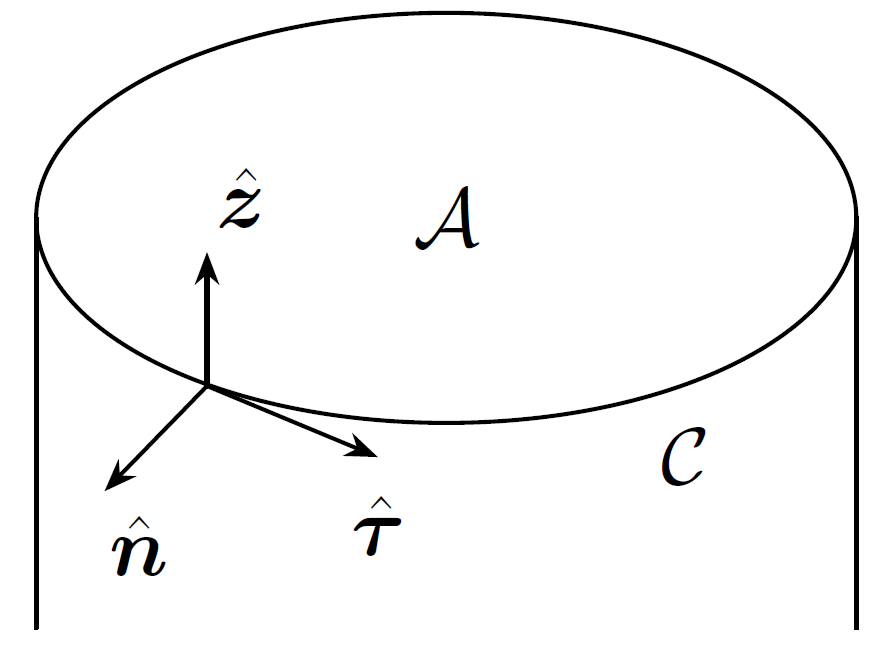
\includegraphics[width=\textwidth]{waveguide_fig/infinitely_long_waveguide_schematic_diagram.png}
		\caption{无限长波导示意图}
		\label{无限长波导示意图}
	\end{minipage}
	\hfill
	\begin{minipage}[b]{0.38\textwidth}
		\centering
		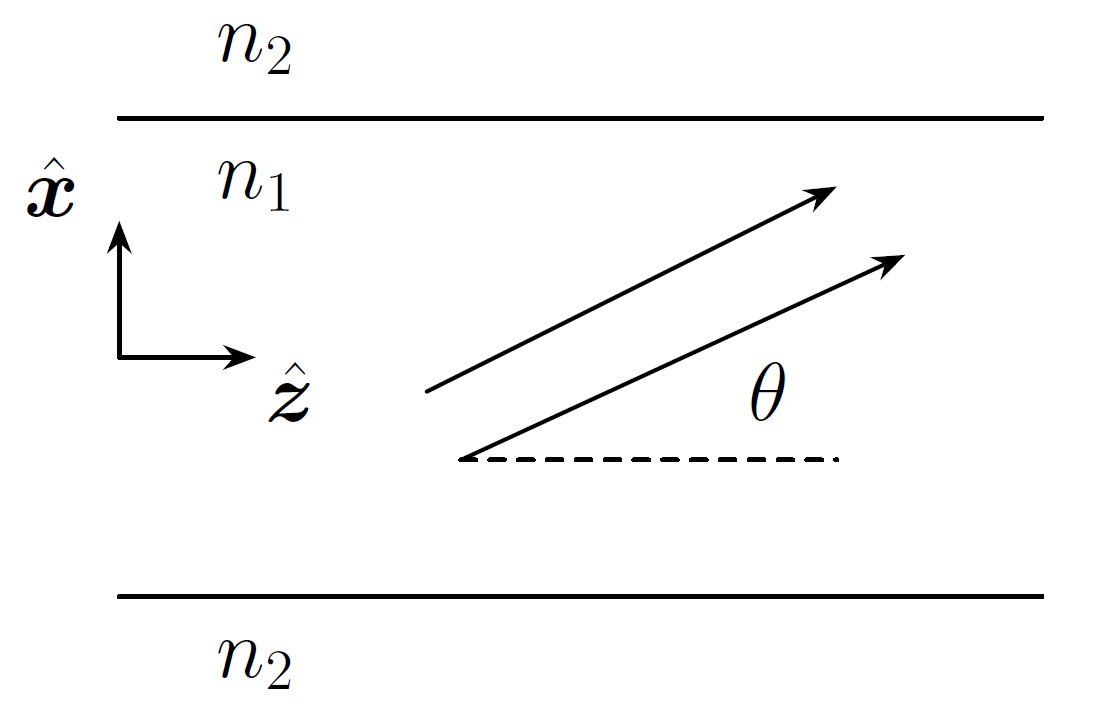
\includegraphics[width=\textwidth]{waveguide_fig/slab_waveguide_schematic_diagram.png}
		\caption{平板波导示意图}
		\label{平板波导示意图}
	\end{minipage}
\end{figure}

\begin{figure}[htbp]
	\centering
	\begin{subfigure}{0.32\textwidth}
		\centering
		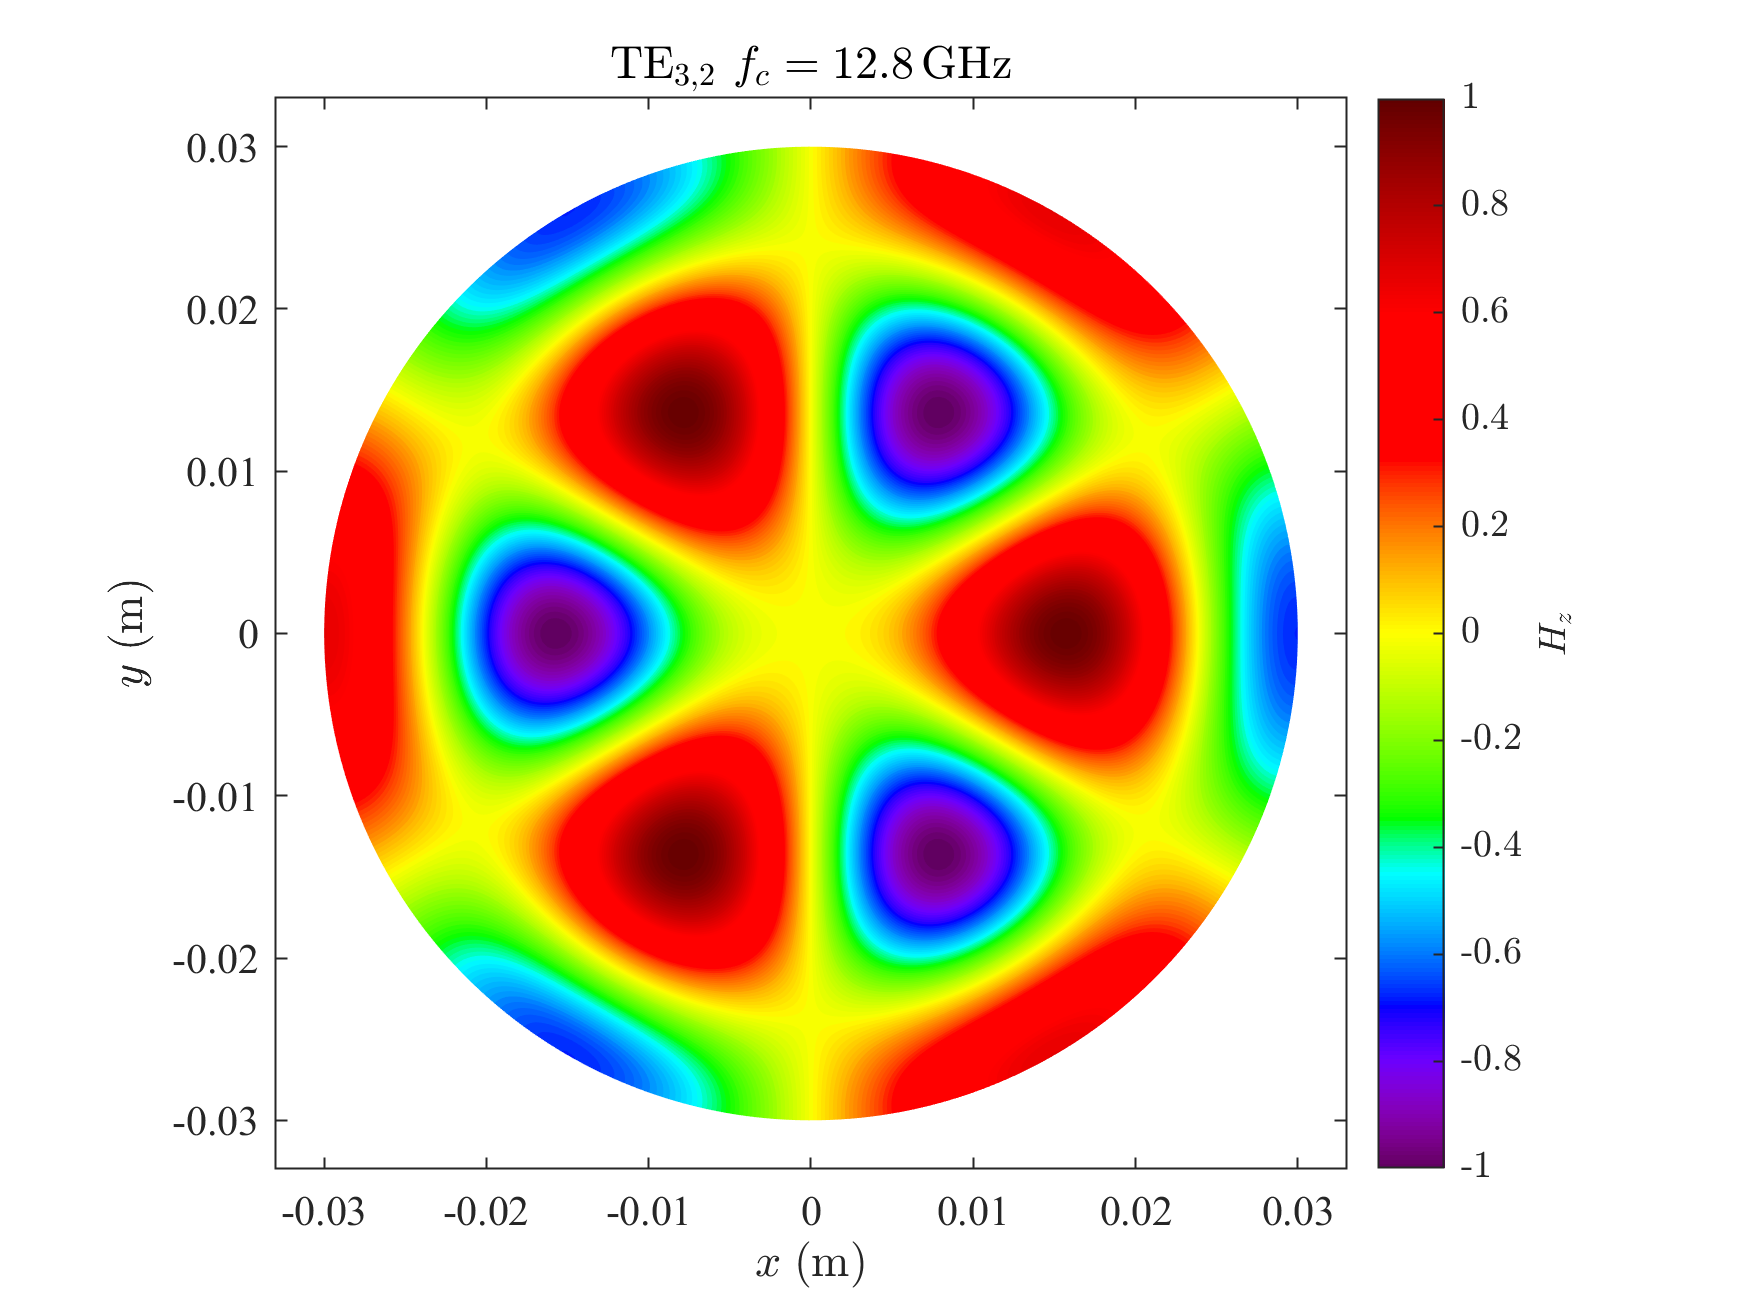
\includegraphics[width=\linewidth]{waveguide_fig/circular_waveguide_te_m3_n2.png}
		\caption{TE, \(m=3\), \(n=2\)}
		\label{圆形波导振幅分布图-TE,m=3,n=2}
	\end{subfigure}
	\hfill
	\begin{subfigure}{0.32\textwidth}
		\centering
		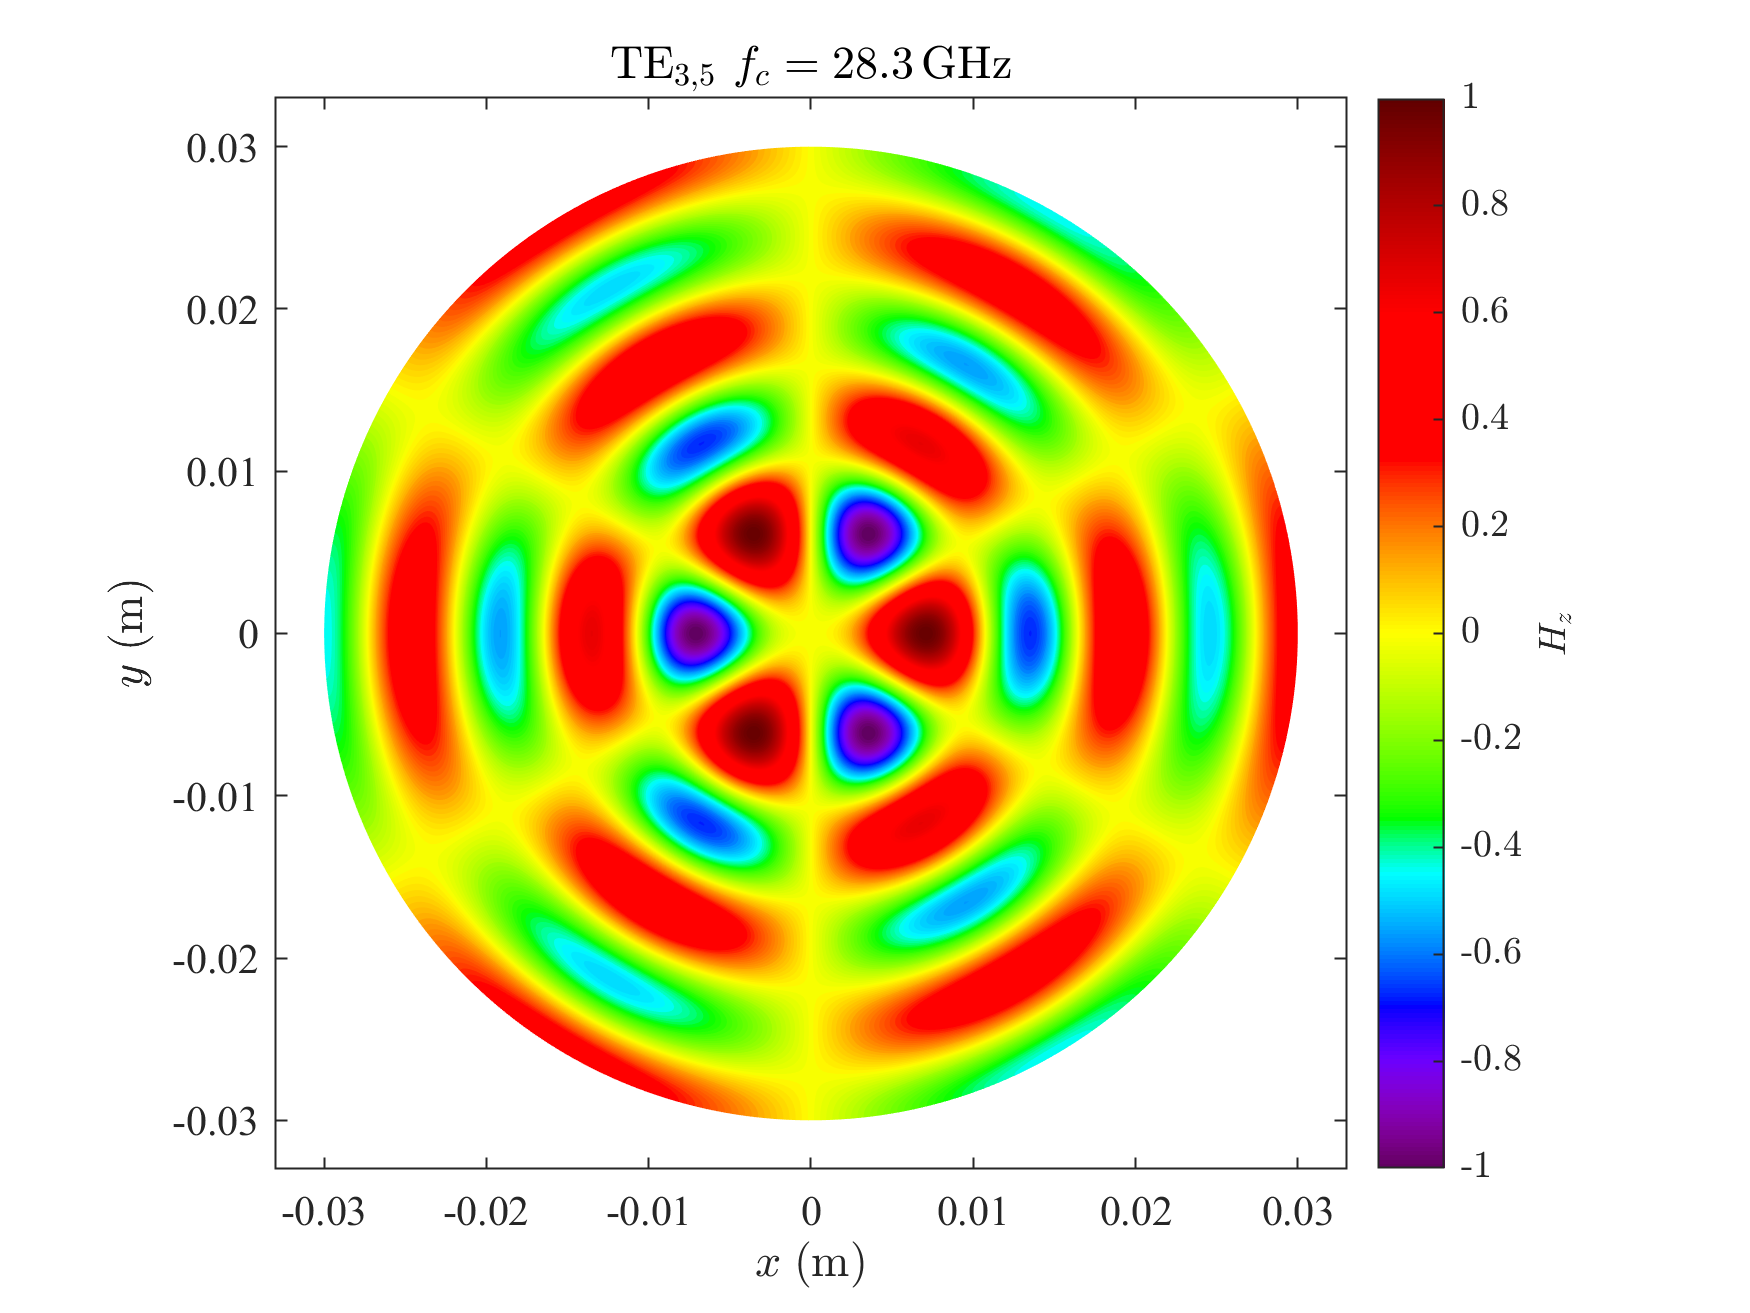
\includegraphics[width=\linewidth]{waveguide_fig/circular_waveguide_te_m3_n5.png}
		\caption{TE, \(m=3\), \(n=5\)}
		\label{圆形波导振幅分布图-TE,m=3,n=5}
	\end{subfigure}
	\hfill
	\begin{subfigure}{0.32\textwidth}
		\centering
		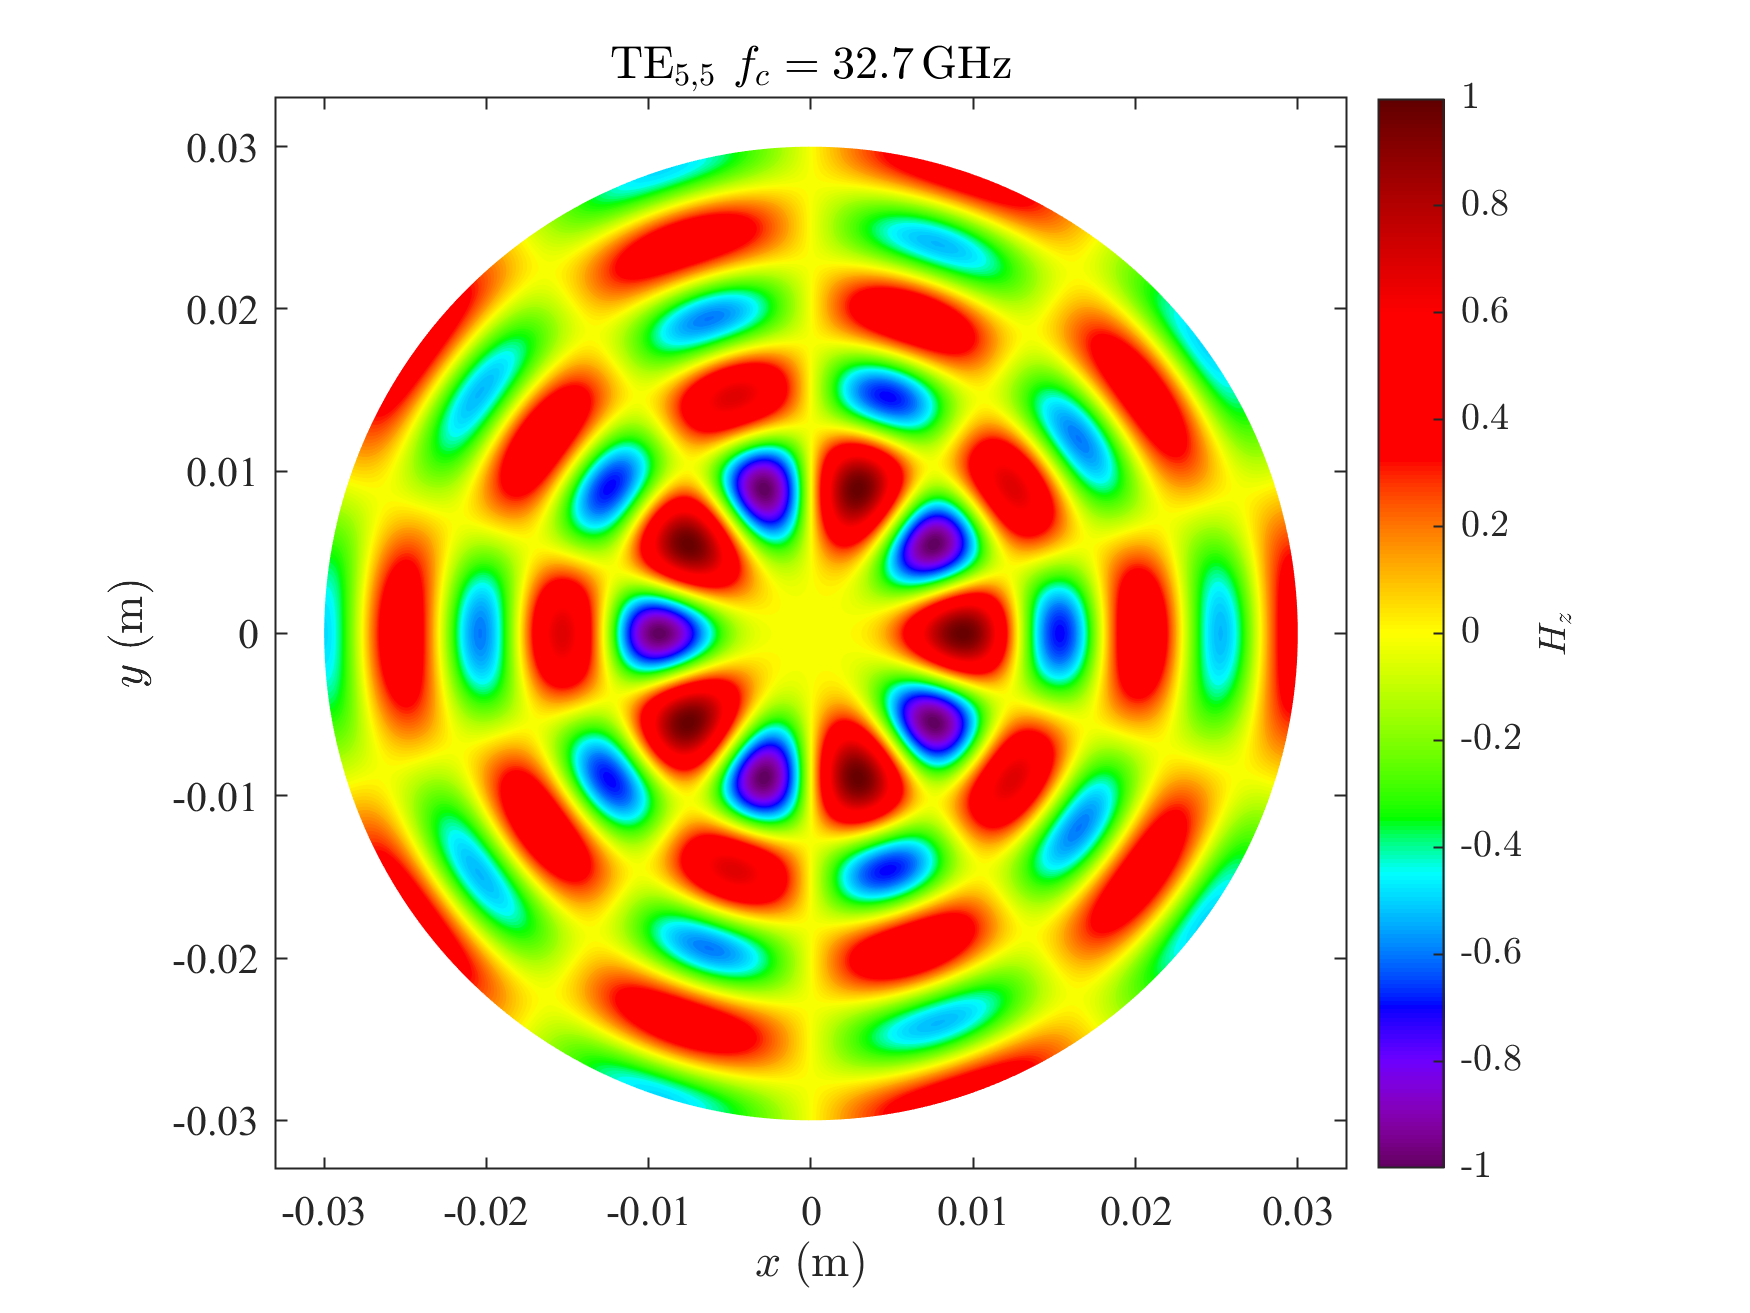
\includegraphics[width=\linewidth]{waveguide_fig/circular_waveguide_te_m5_n5.png}
		\caption{TE, \(m=5\), \(n=5\)}
		\label{圆形波导振幅分布图-TE,m=5,n=5}
	\end{subfigure}

	\vspace{1em}

	\begin{subfigure}{0.32\textwidth}
		\centering
		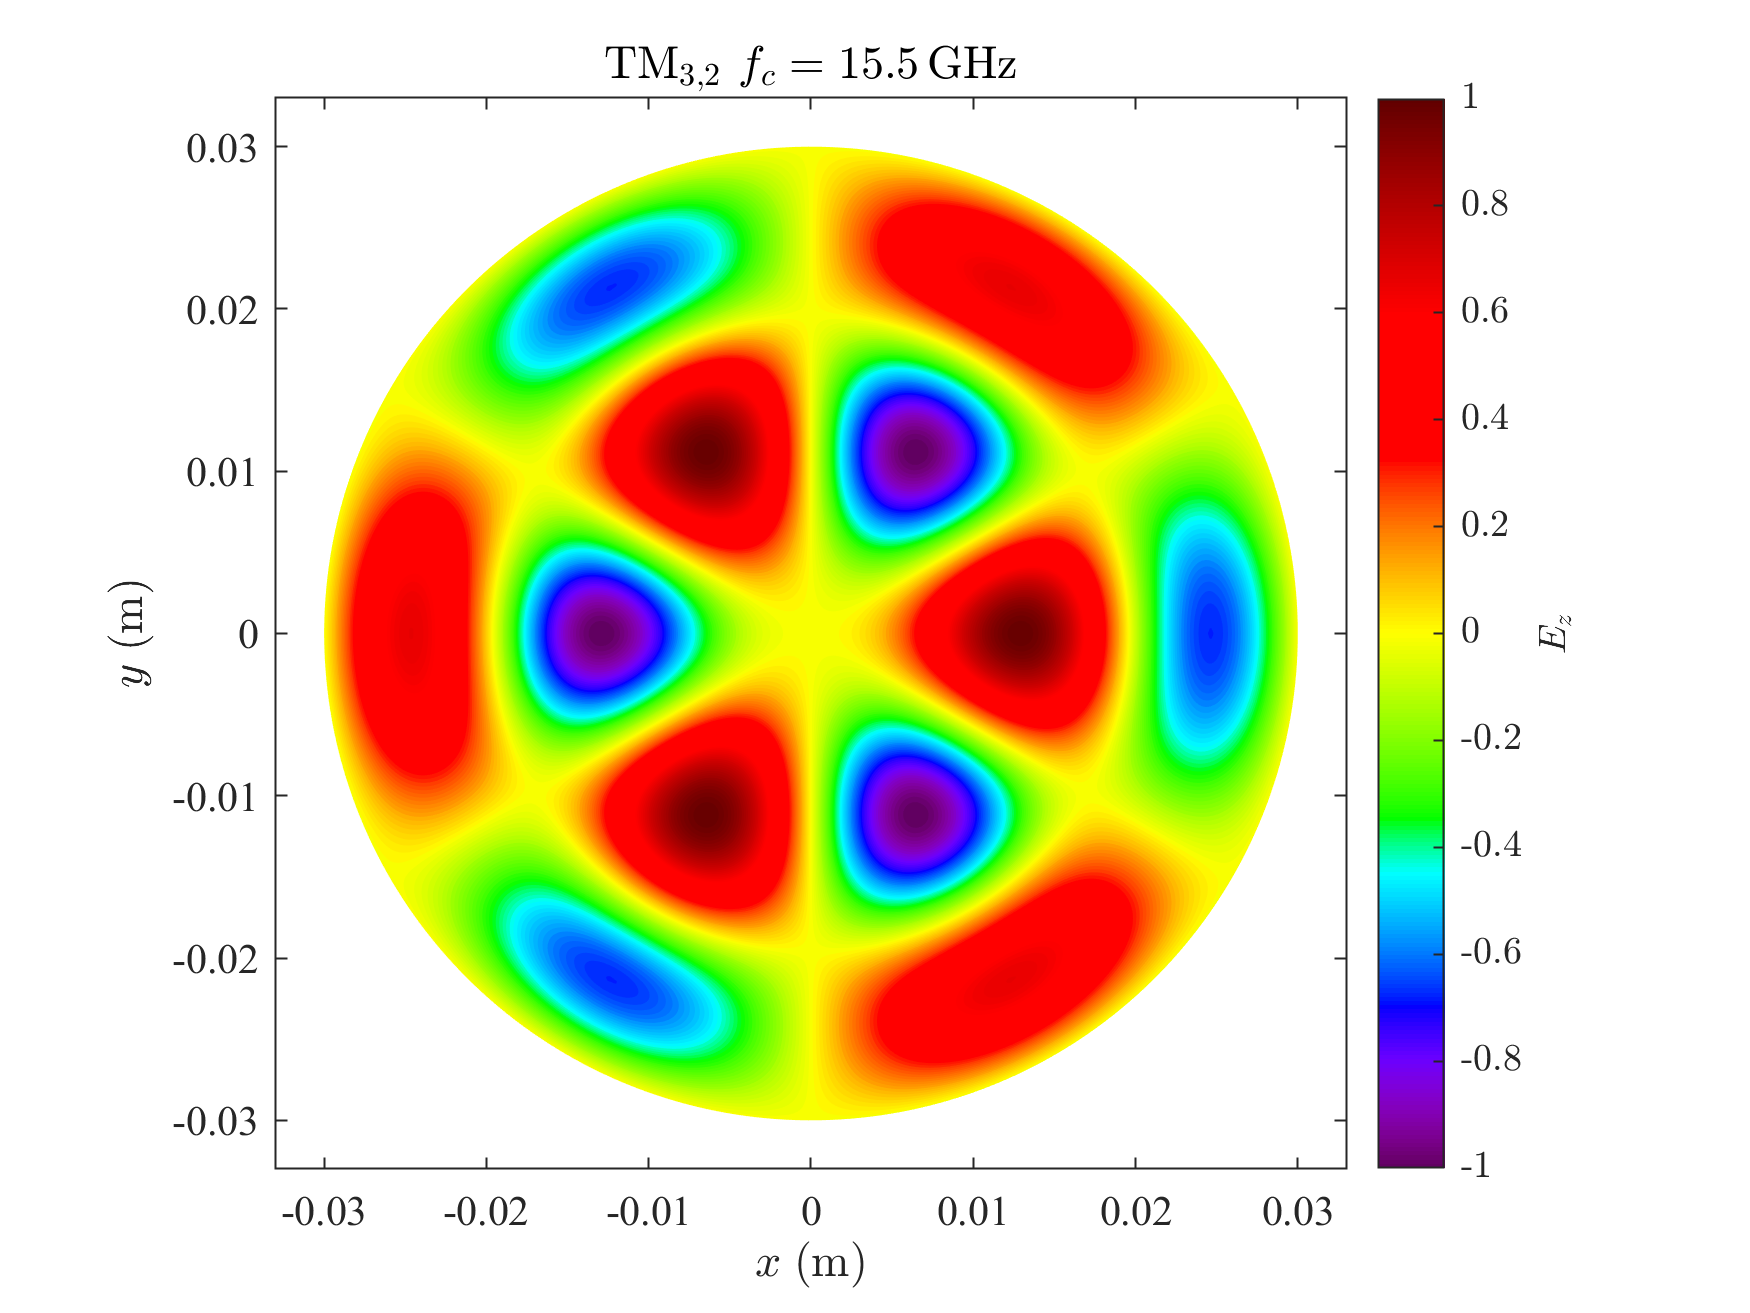
\includegraphics[width=\linewidth]{waveguide_fig/circular_waveguide_tm_m3_n2.png}
		\caption{TM, \(m=3\), \(n=2\)}
		\label{圆形波导振幅分布图-TM,m=3,n=2}
	\end{subfigure}
	\hfill
	\begin{subfigure}{0.32\textwidth}
		\centering
		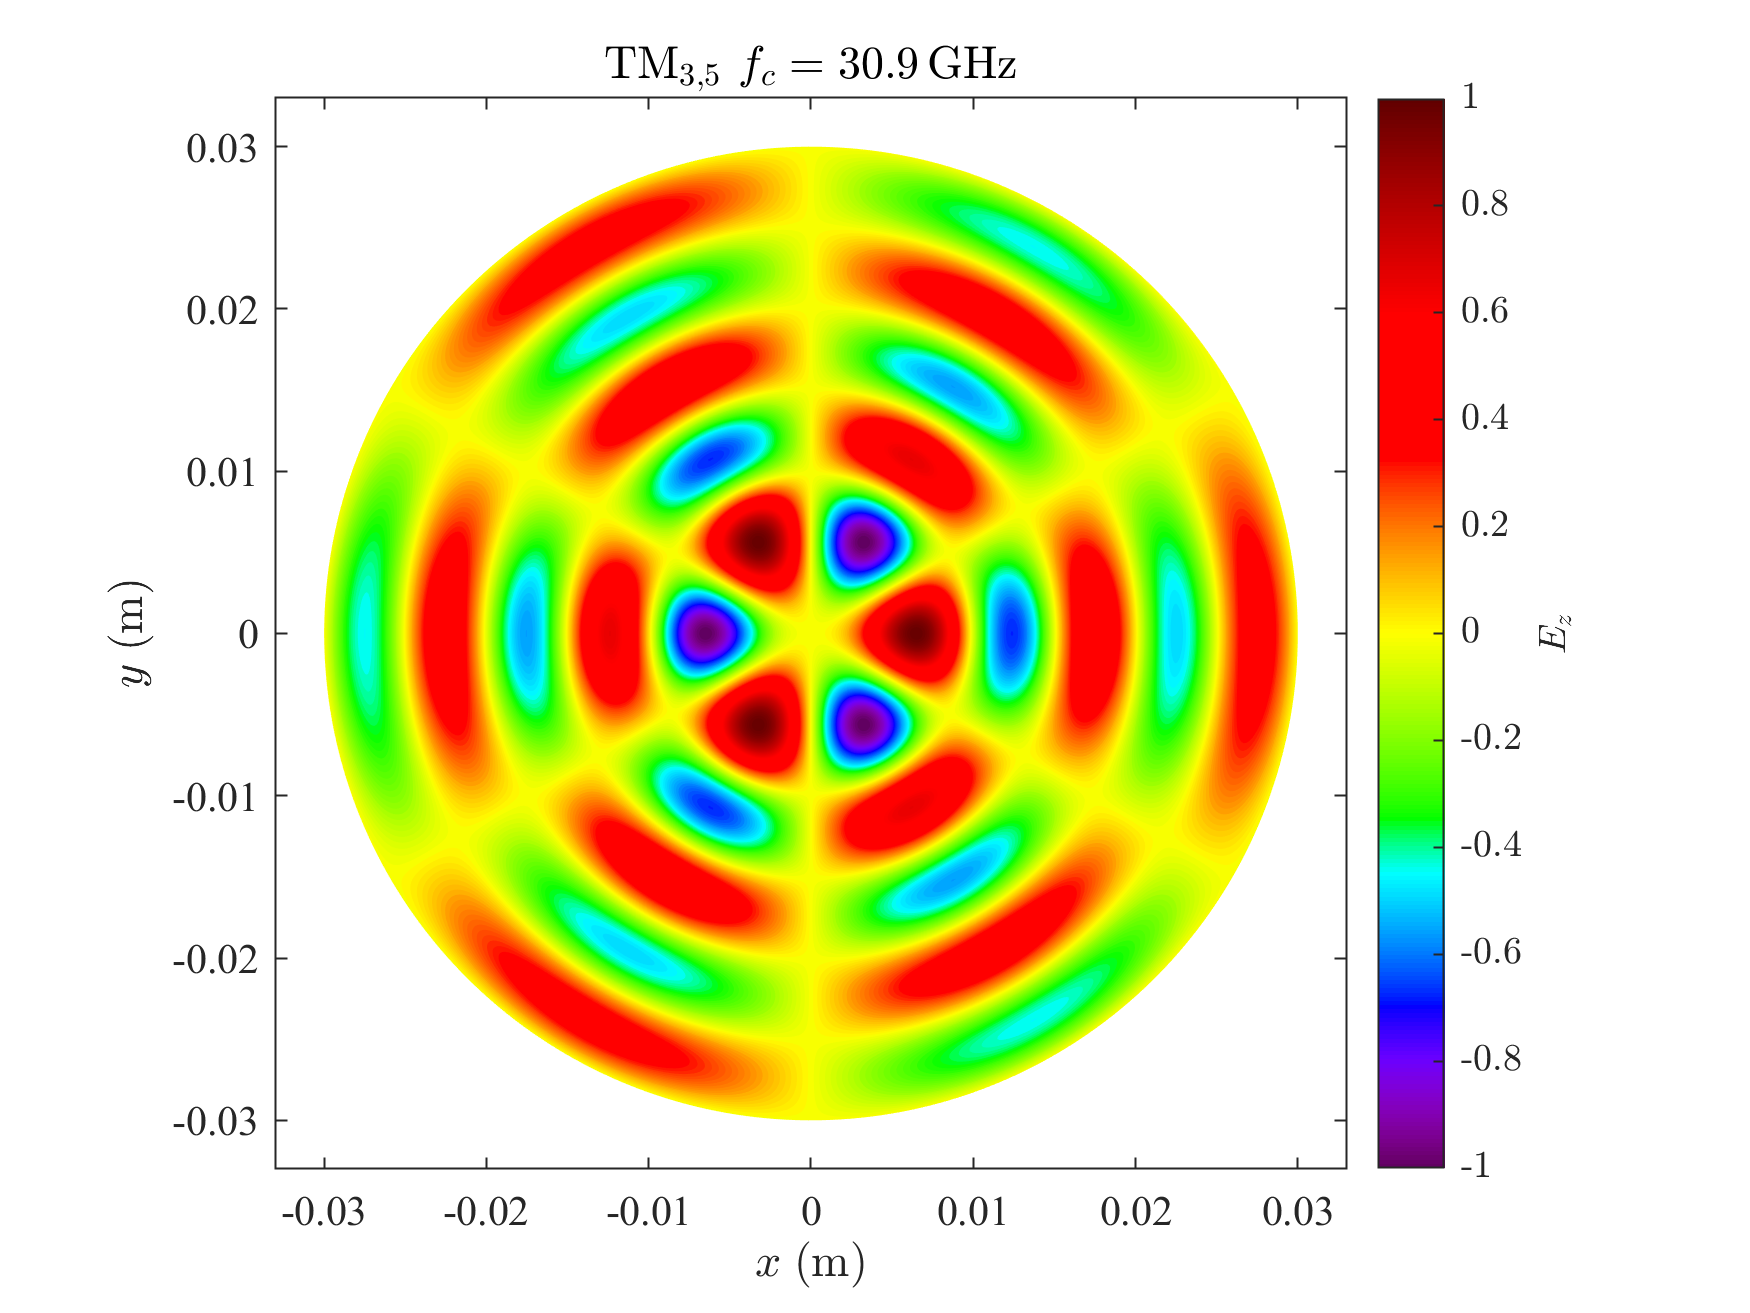
\includegraphics[width=\linewidth]{waveguide_fig/circular_waveguide_tm_m3_n5.png}
		\caption{TM, \(m=3\), \(n=5\)}
		\label{圆形波导振幅分布图-TM,m=3,n=5}
	\end{subfigure}
	\hfill
	\begin{subfigure}{0.32\textwidth}
		\centering
		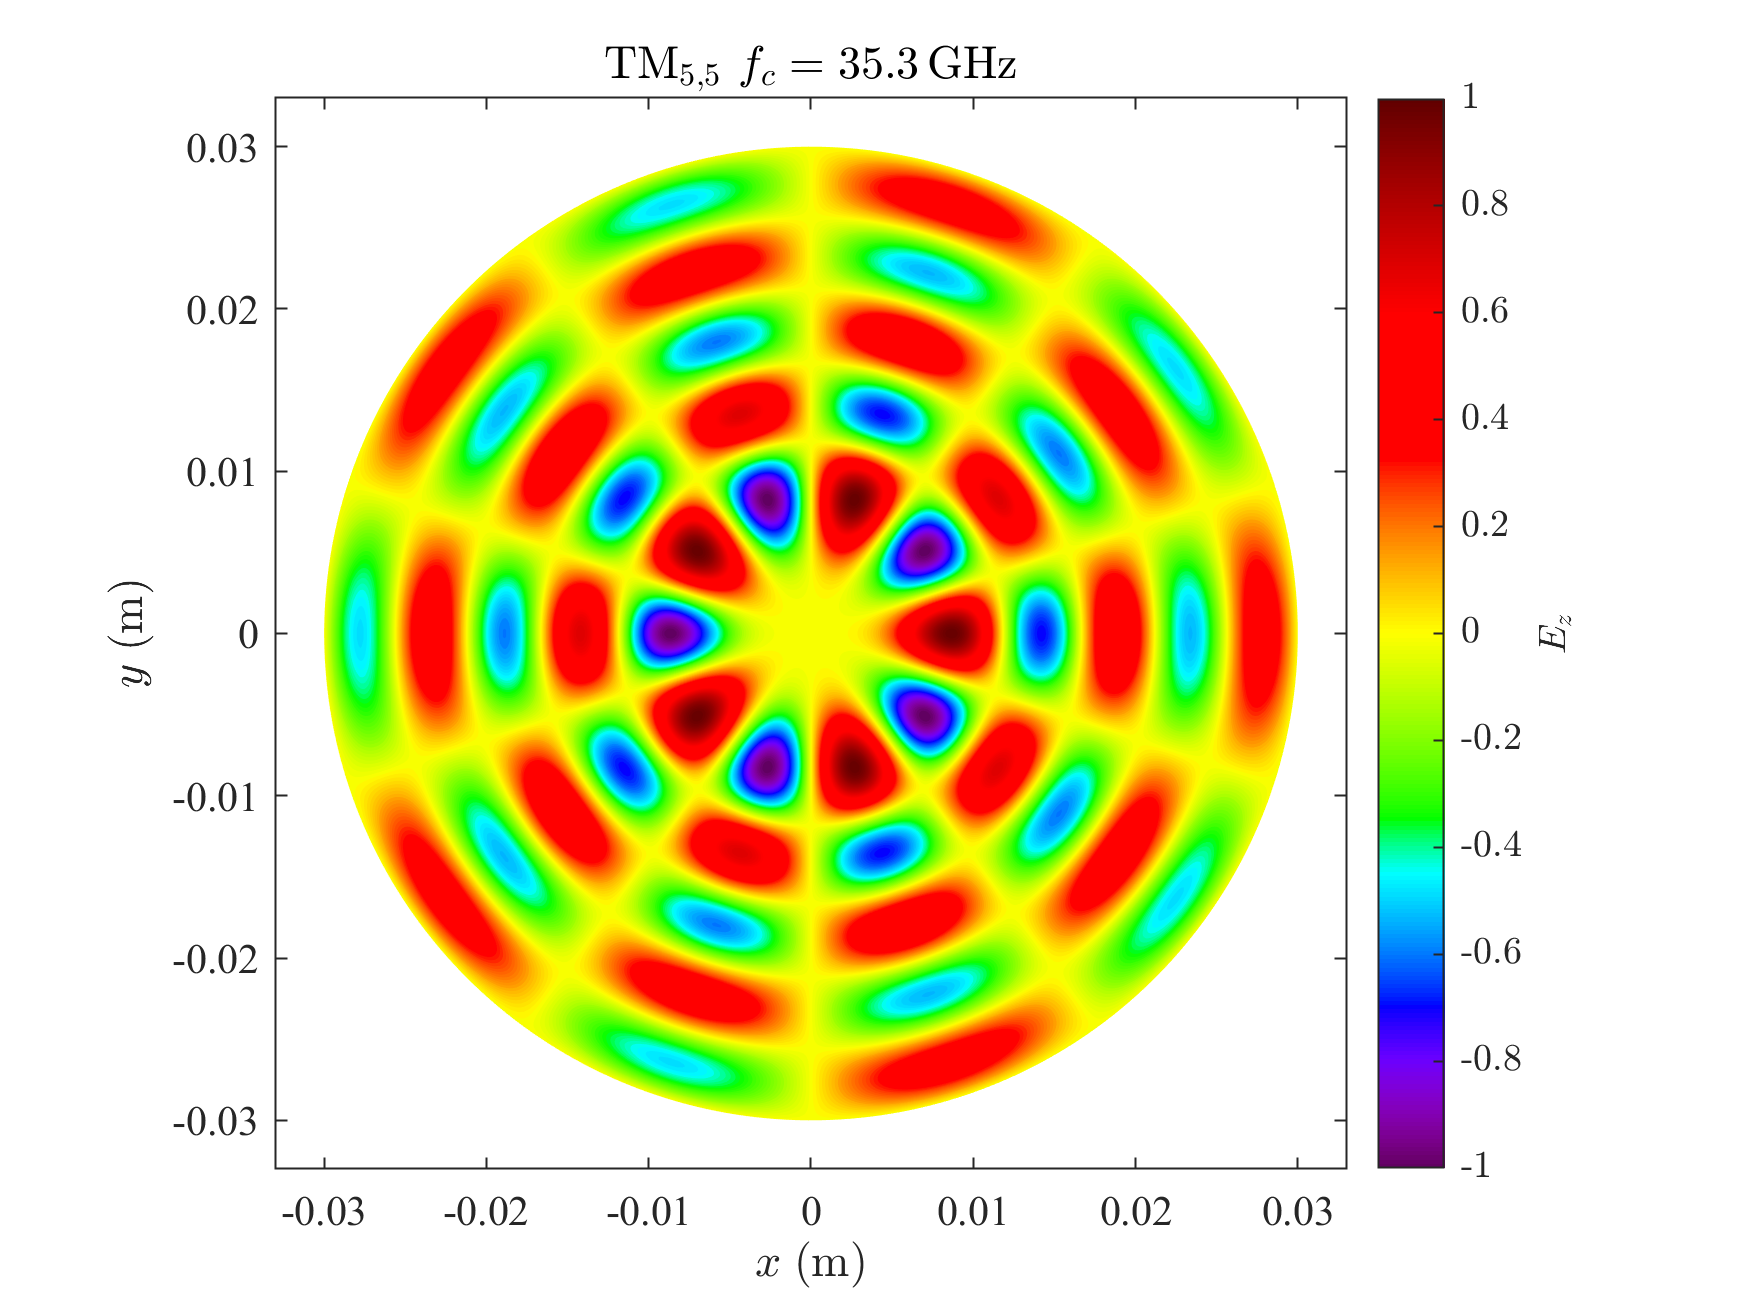
\includegraphics[width=\linewidth]{waveguide_fig/circular_waveguide_tm_m5_n5.png}
		\caption{TM, \(m=5\), \(n=5\)}
		\label{圆形波导振幅分布图-TM,m=5,n=5}
	\end{subfigure}
	\caption{圆形波导振幅分布图}
	\label{圆形波导振幅分布图}
\end{figure}

\begin{figure}[htbp]
	\centering
	\begin{subfigure}{0.32\textwidth}
		\centering
		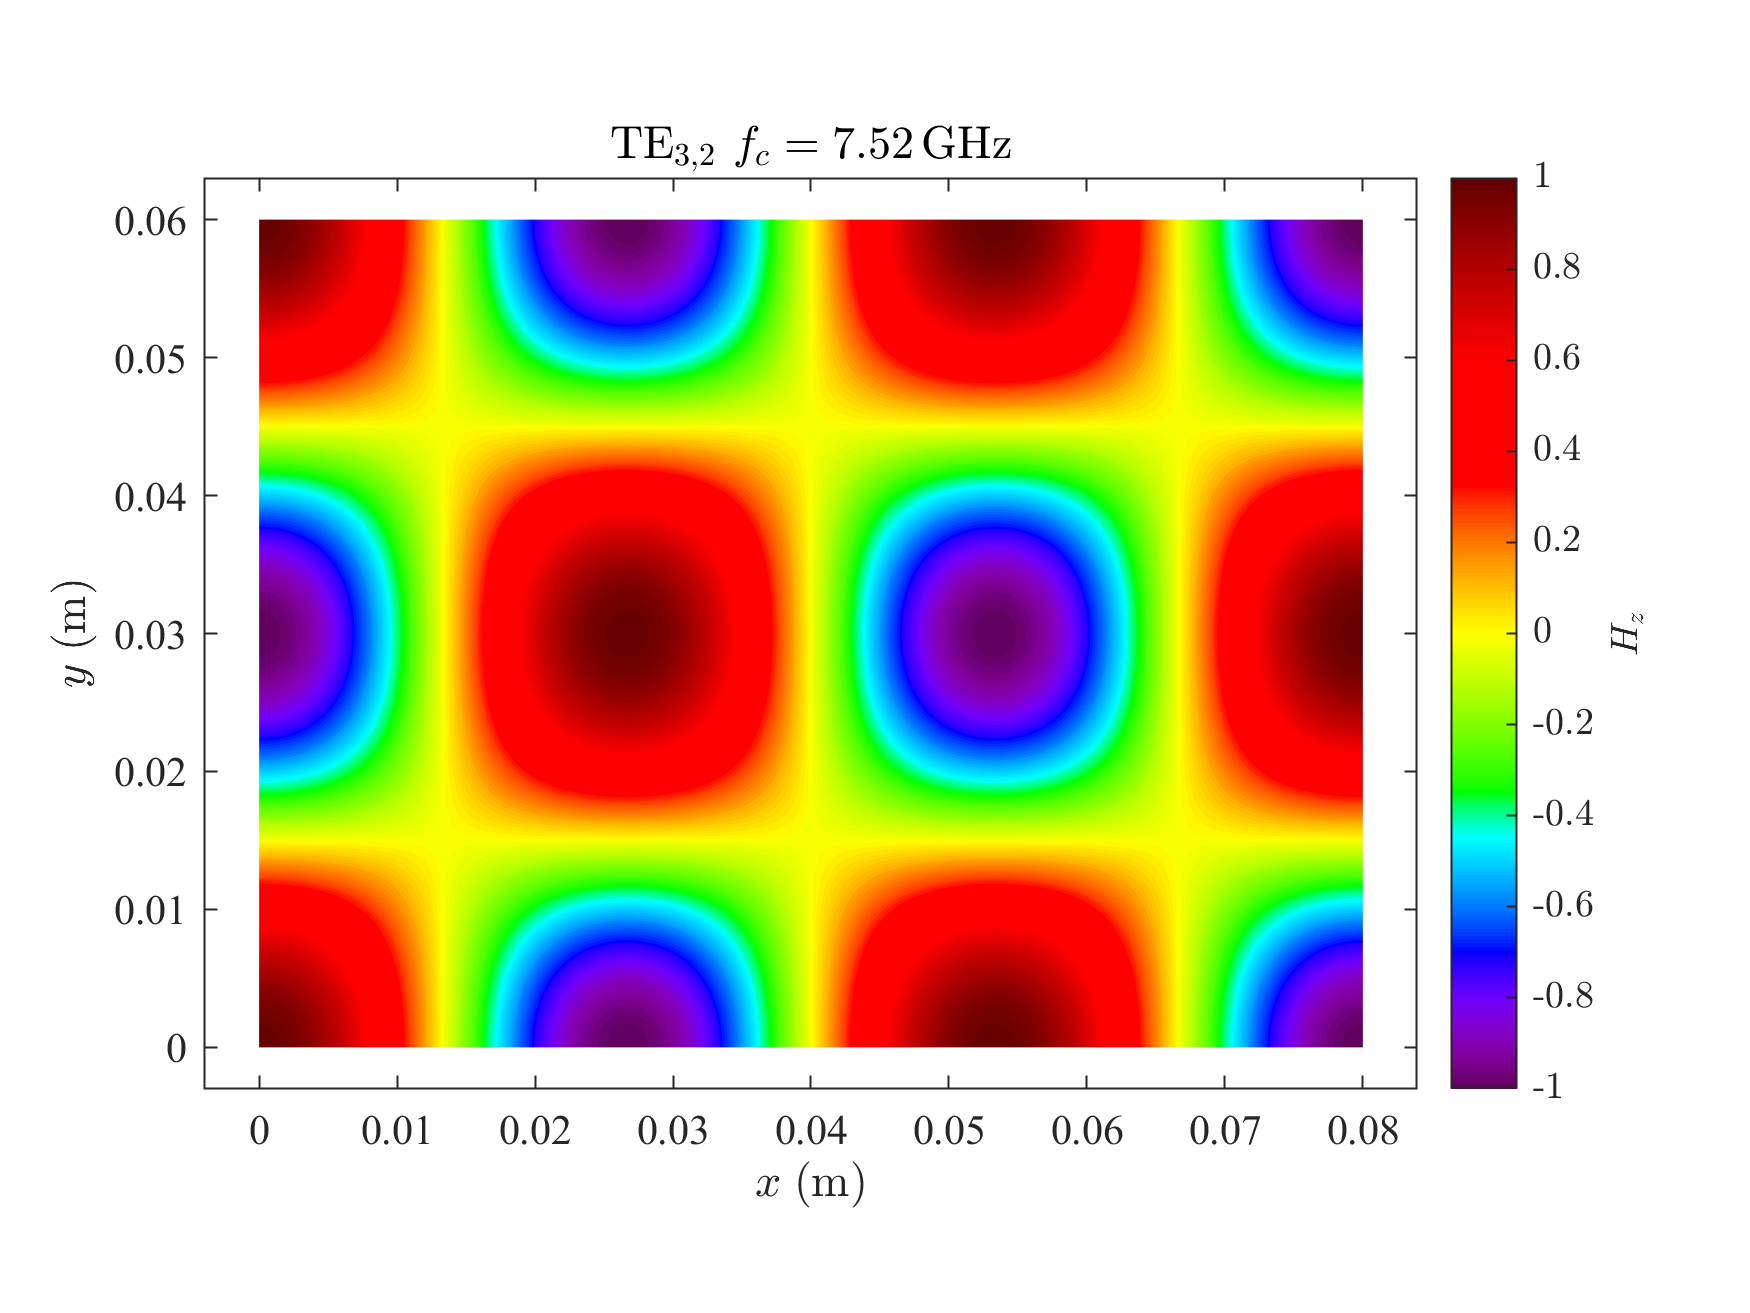
\includegraphics[width=\linewidth]{waveguide_fig/rectangular_waveguide_te_m3_n2.png}
		\caption{TE, \(m=3\), \(n=2\)}
		\label{矩形波导振幅分布图-TE,m=3,n=2}
	\end{subfigure}
	\hfill
	\begin{subfigure}{0.32\textwidth}
		\centering
		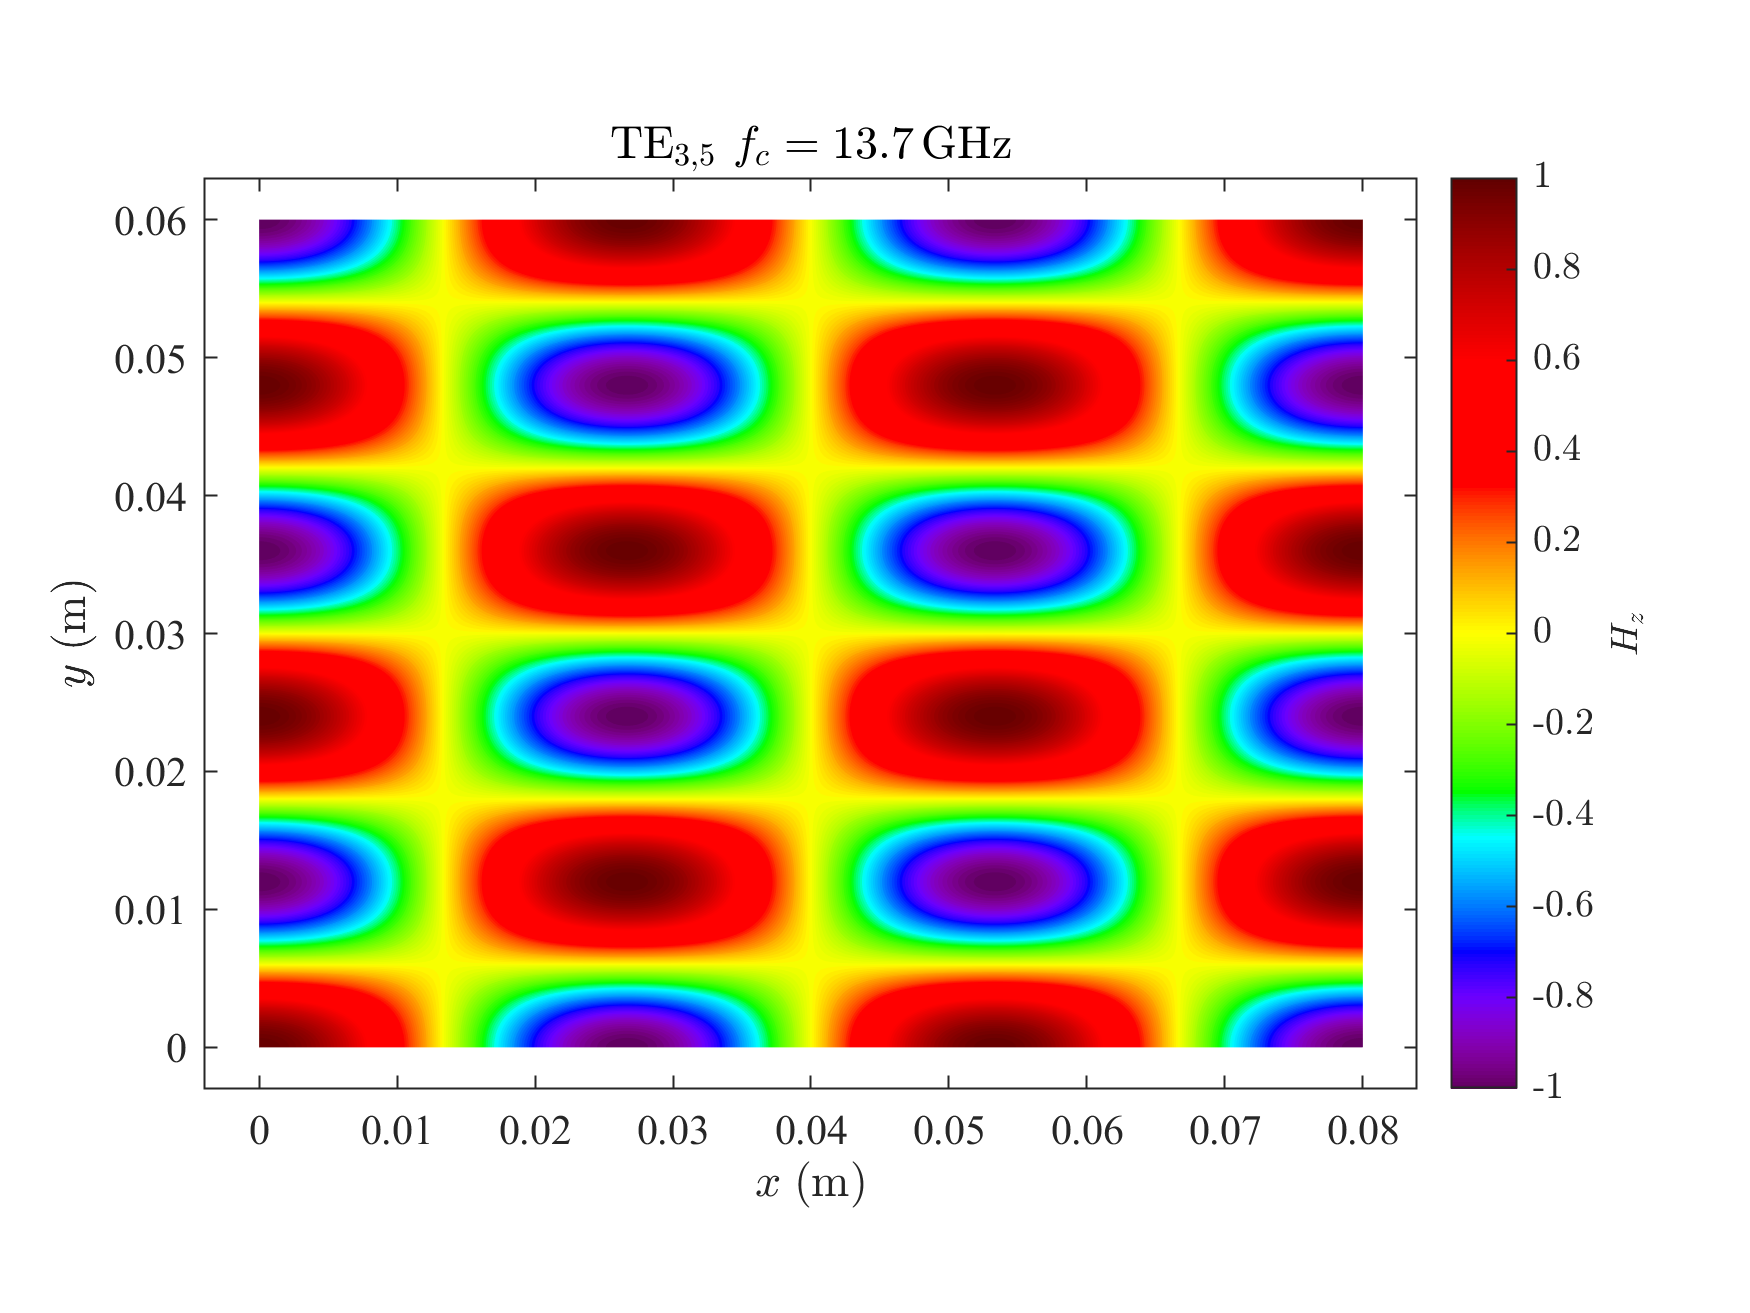
\includegraphics[width=\linewidth]{waveguide_fig/rectangular_waveguide_te_m3_n5.png}
		\caption{TE, \(m=3\), \(n=5\)}
		\label{矩形波导振幅分布图-TE,m=3,n=5}
	\end{subfigure}
	\hfill
	\begin{subfigure}{0.32\textwidth}
		\centering
		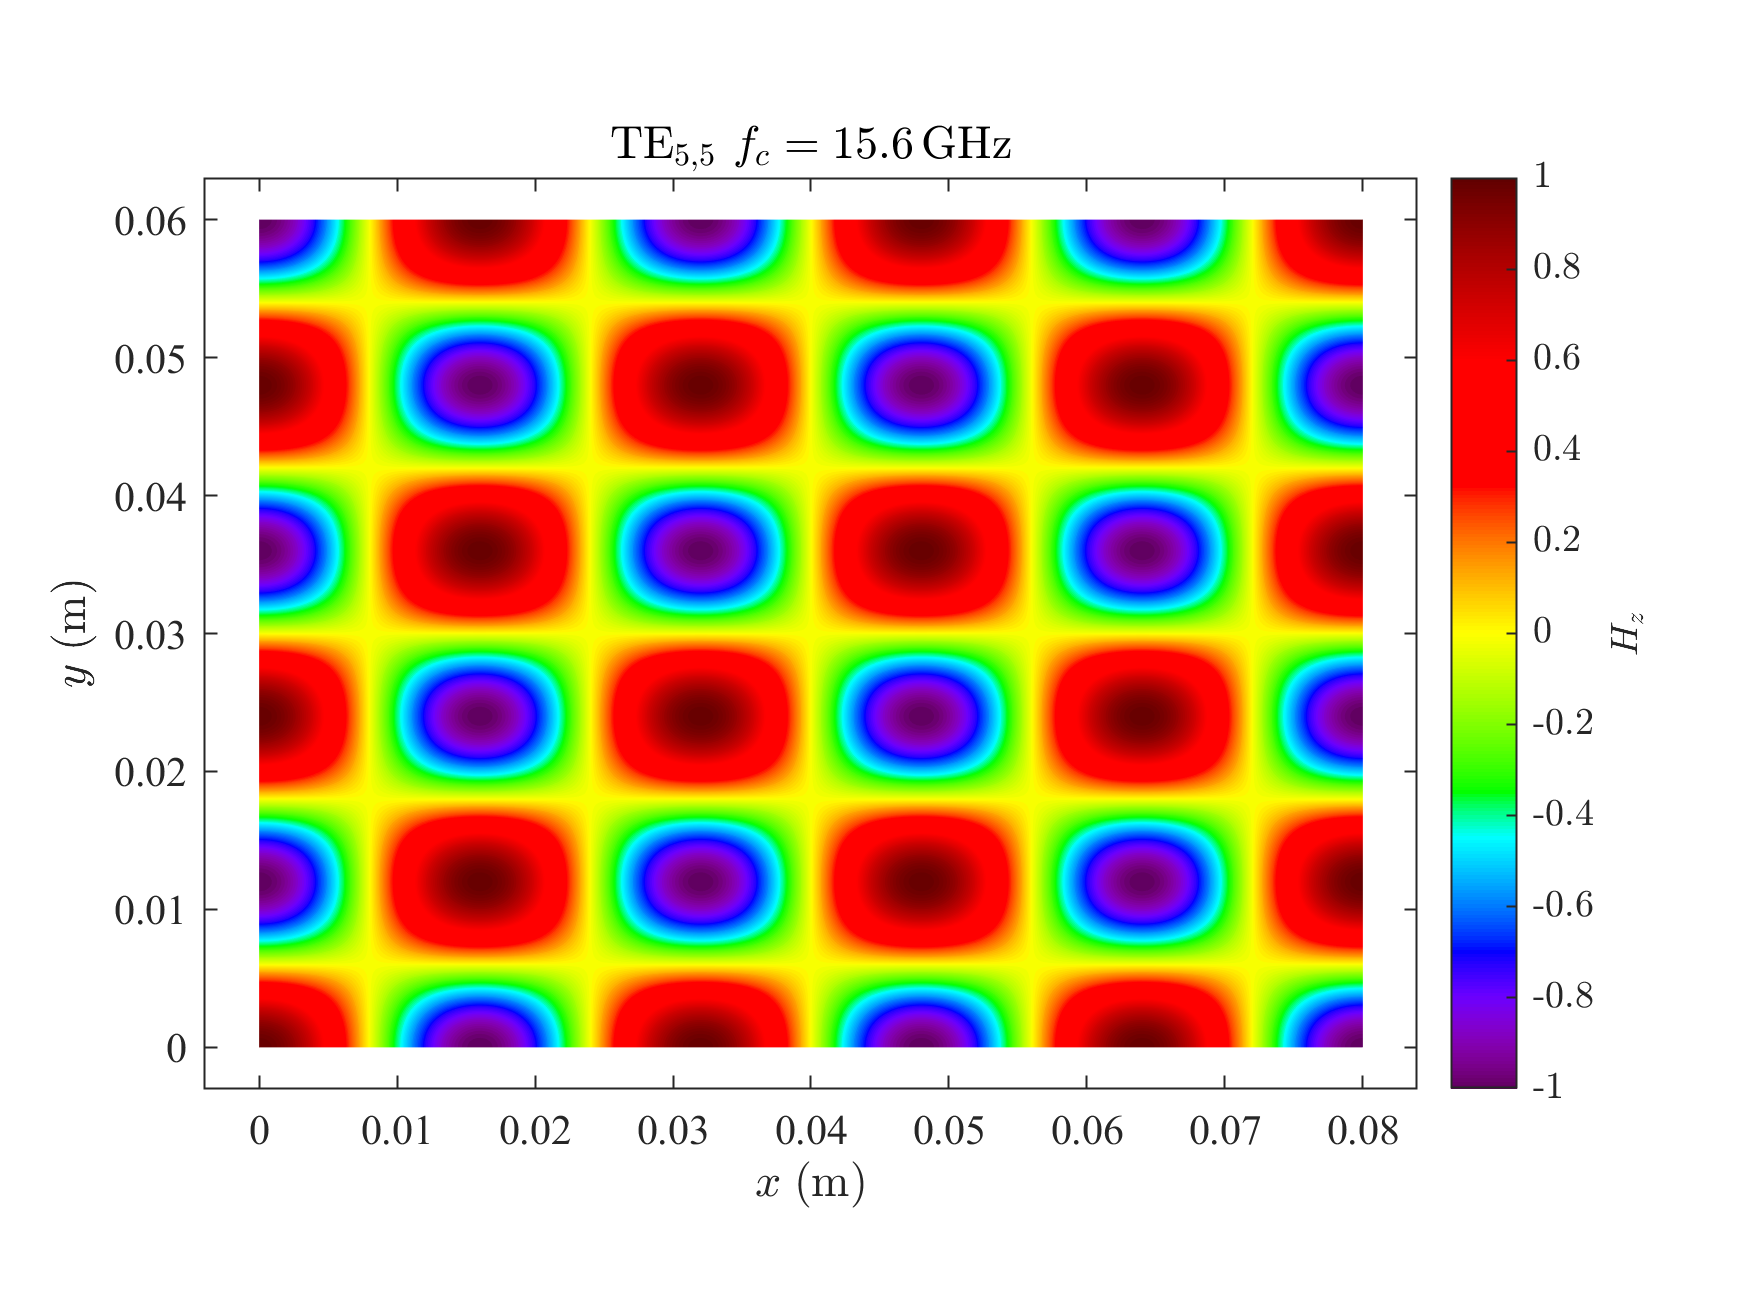
\includegraphics[width=\linewidth]{waveguide_fig/rectangular_waveguide_te_m5_n5.png}
		\caption{TE, \(m=5\), \(n=5\)}
		\label{矩形波导振幅分布图-TE,m=5,n=5}
	\end{subfigure}

	\vspace{1em}

	\begin{subfigure}{0.32\textwidth}
		\centering
		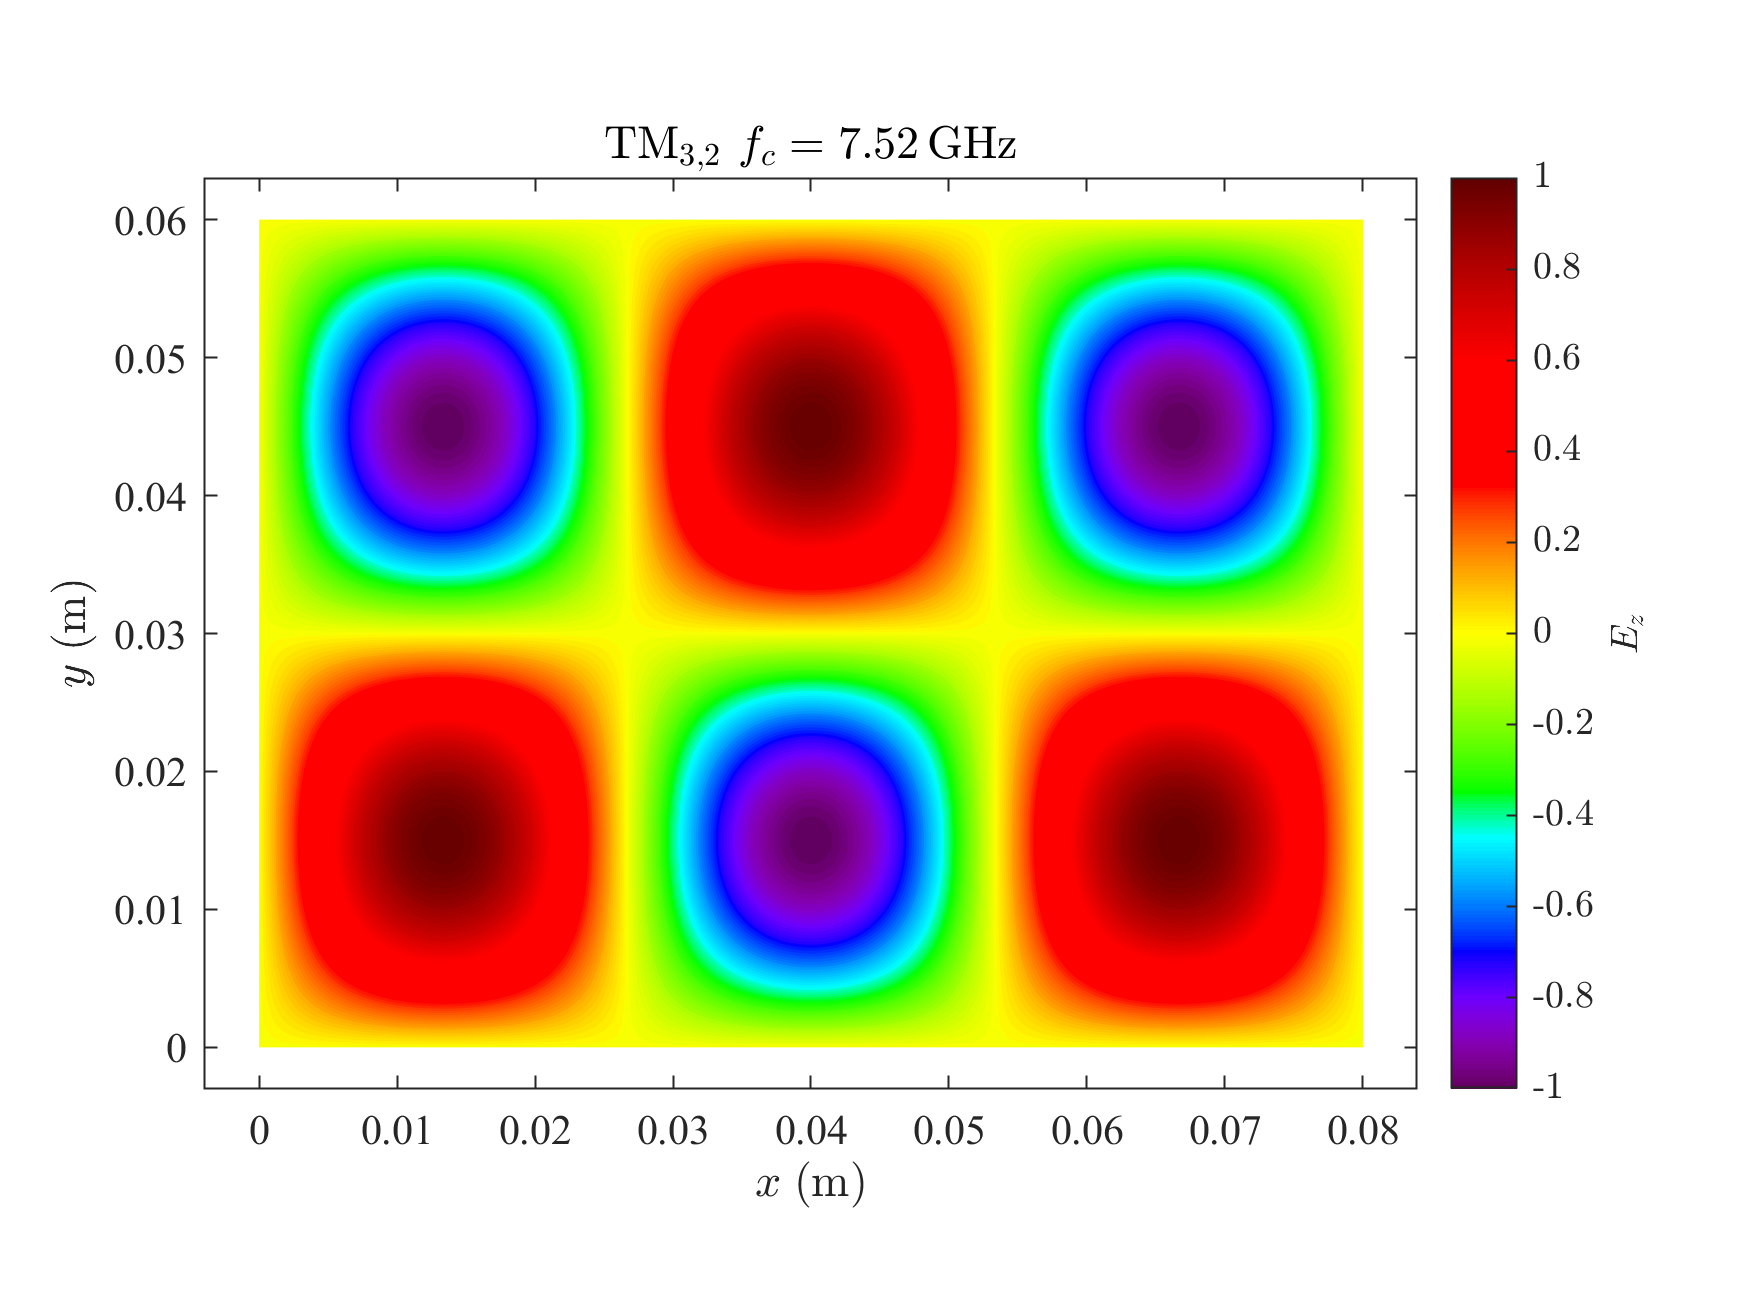
\includegraphics[width=\linewidth]{waveguide_fig/rectangular_waveguide_tm_m3_n2.png}
		\caption{TM, \(m=3\), \(n=2\)}
		\label{矩形波导振幅分布图-TM,m=3,n=2}
	\end{subfigure}
	\hfill
	\begin{subfigure}{0.32\textwidth}
		\centering
		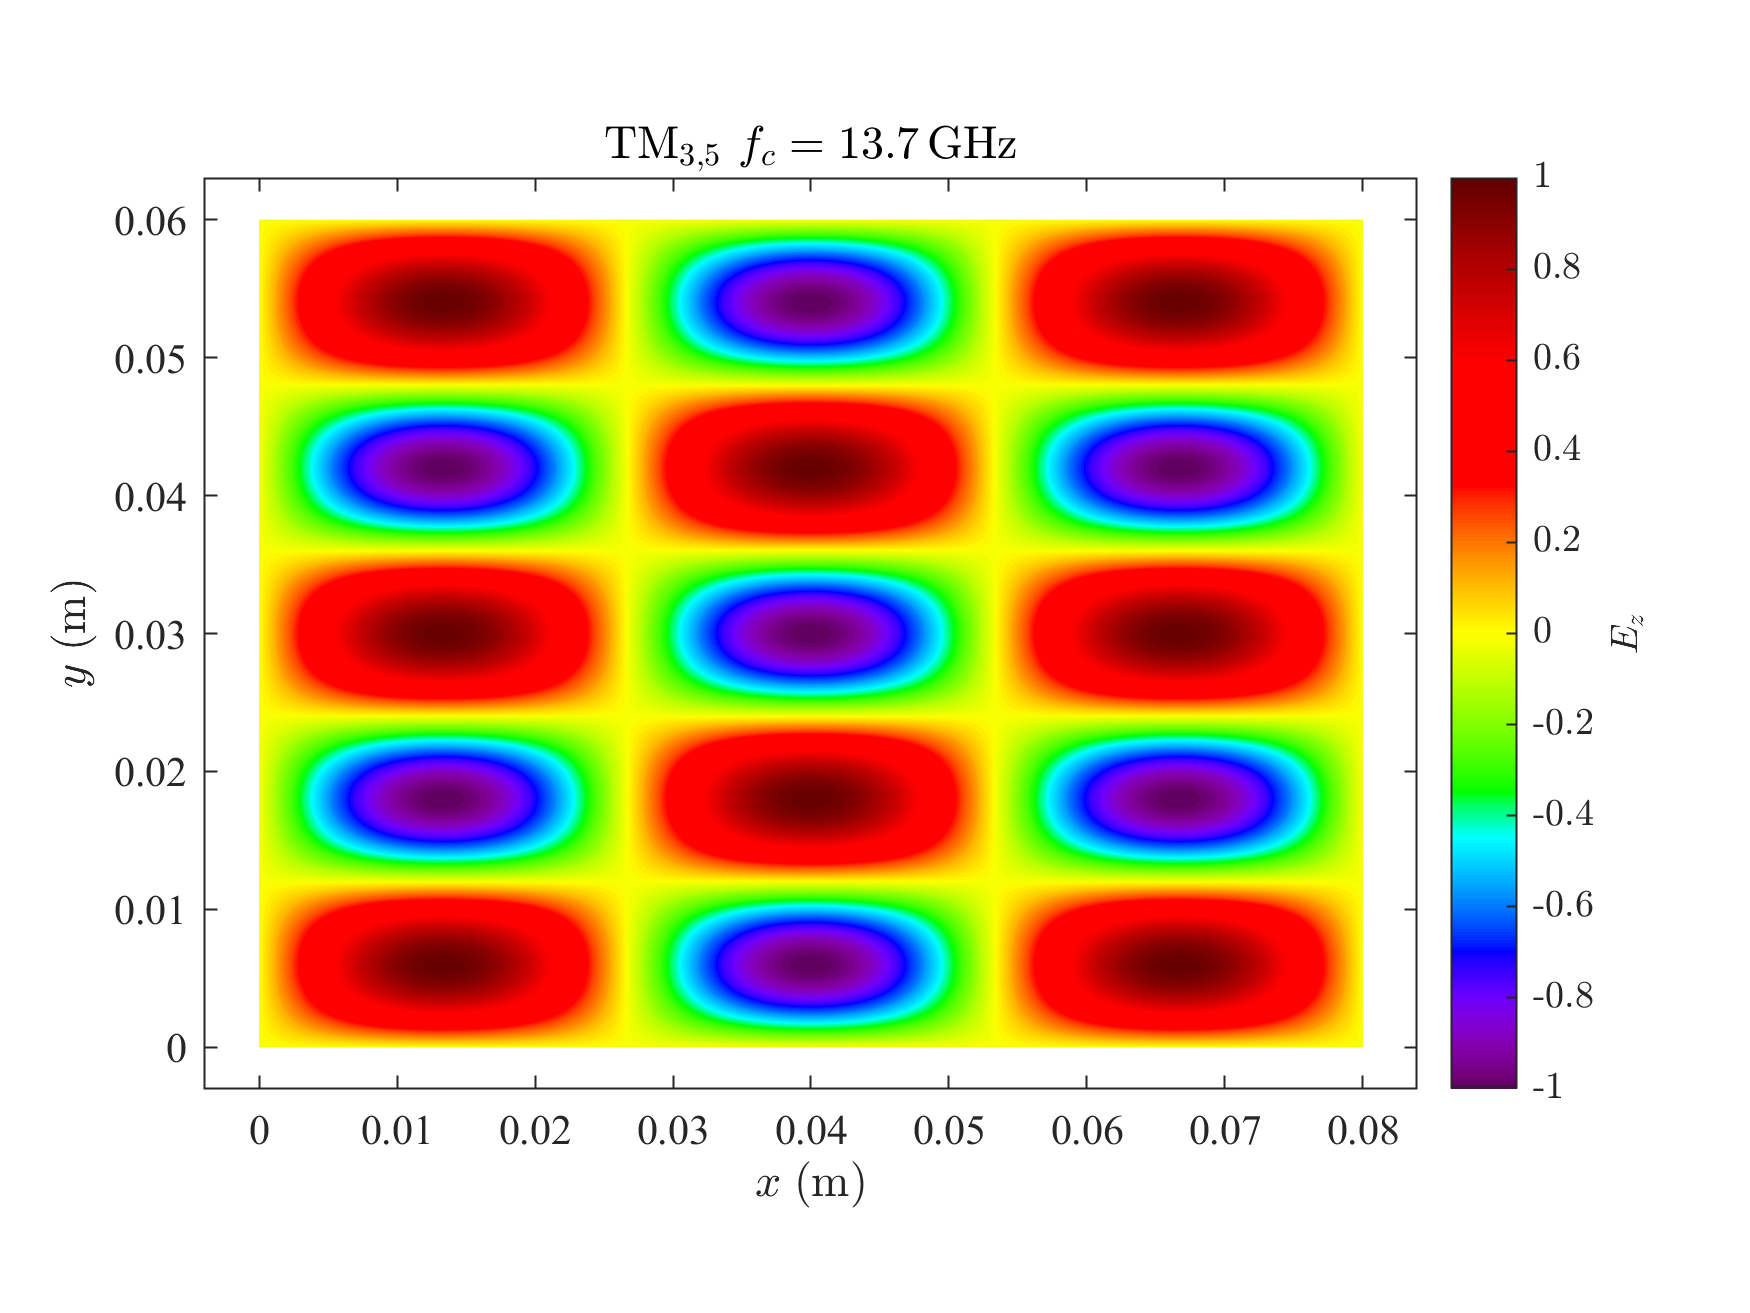
\includegraphics[width=\linewidth]{waveguide_fig/rectangular_waveguide_tm_m3_n5.png}
		\caption{TM, \(m=3\), \(n=5\)}
		\label{矩形波导振幅分布图-TM,m=3,n=5}
	\end{subfigure}
	\hfill
	\begin{subfigure}{0.32\textwidth}
		\centering
		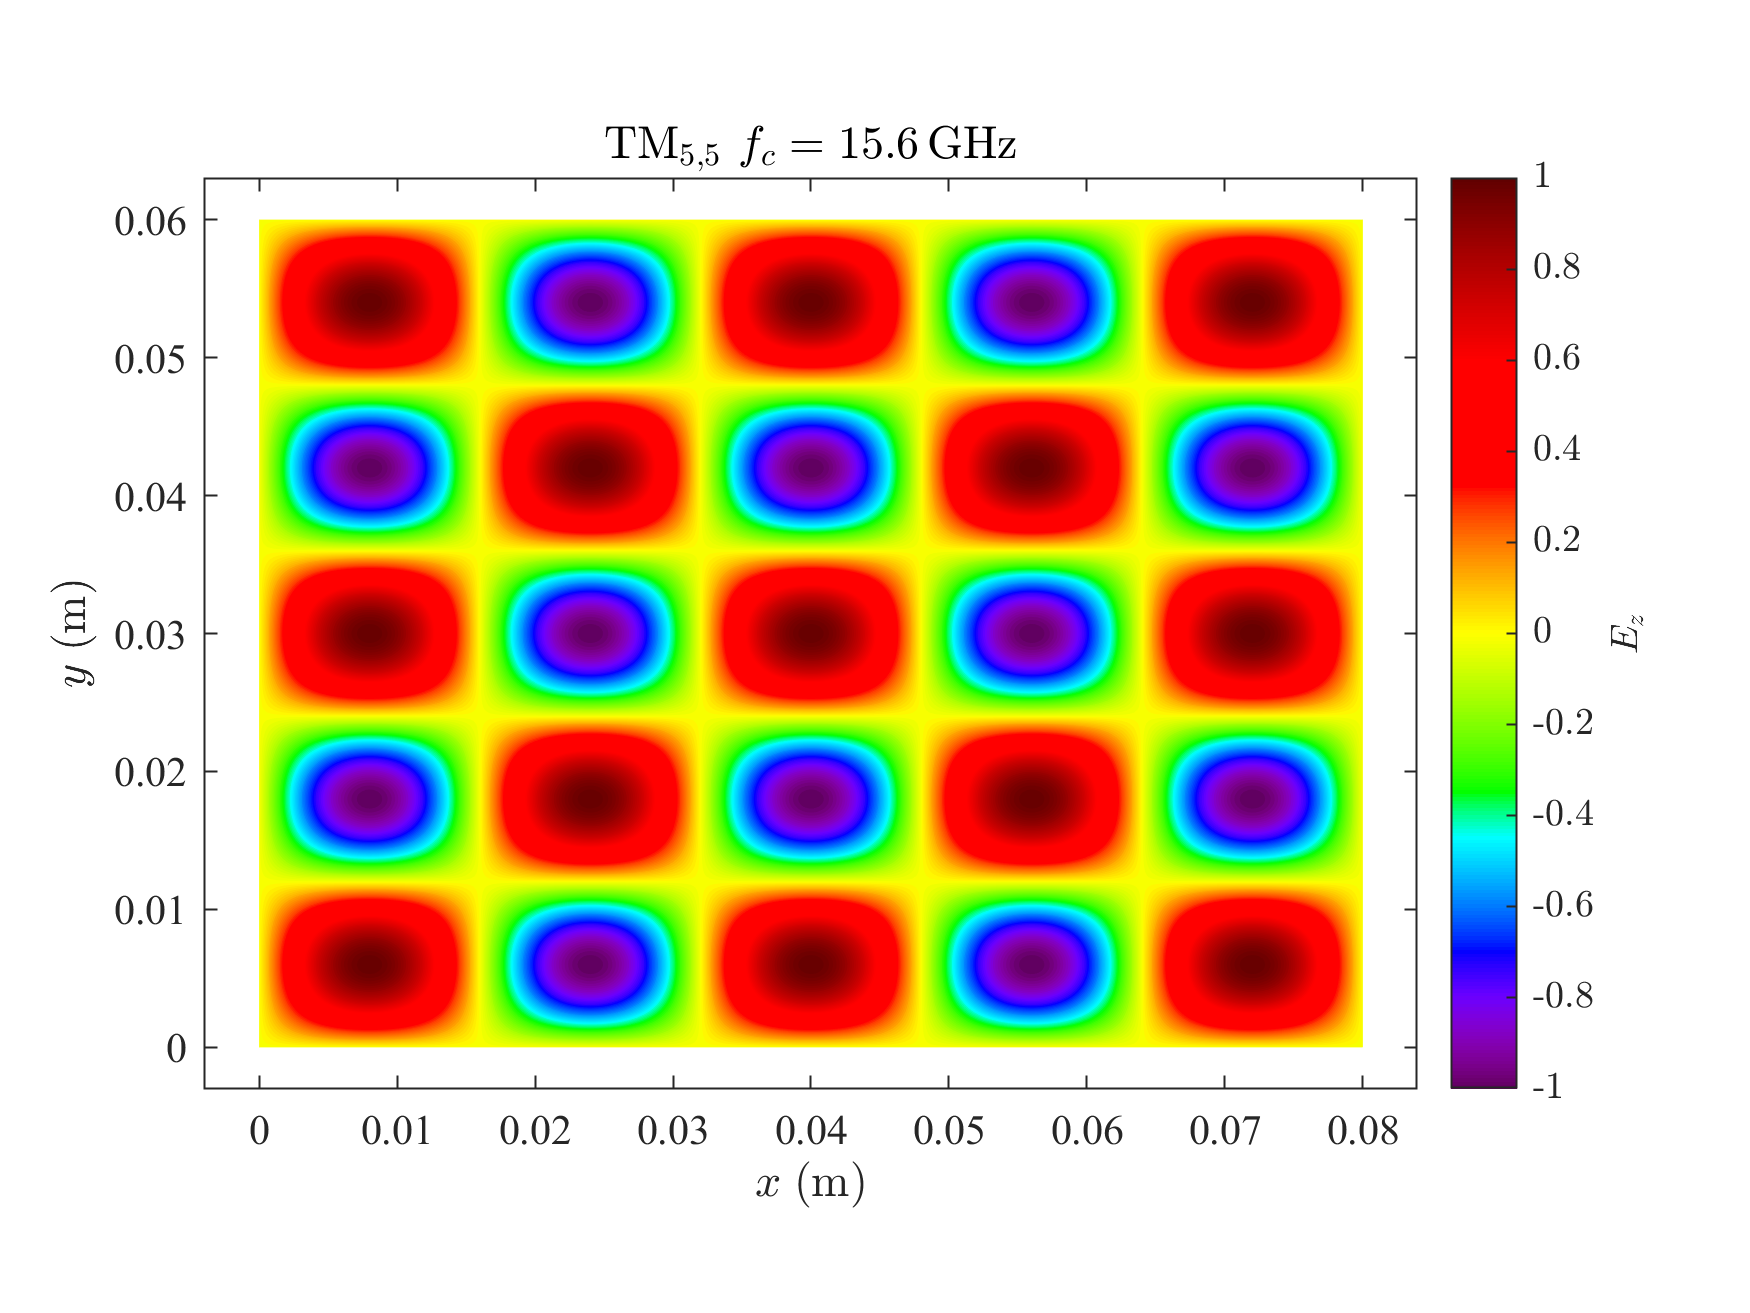
\includegraphics[width=\linewidth]{waveguide_fig/rectangular_waveguide_tm_m5_n5.png}
		\caption{TM, \(m=5\), \(n=5\)}
		\label{矩形波导振幅分布图-TM,m=5,n=5}
	\end{subfigure}
	\caption{矩形波导振幅分布图}
	\label{矩形波导振幅分布图}
\end{figure}

\begin{figure}[htbp]
	\centering
	\begin{subfigure}{0.32\textwidth}
		\centering
		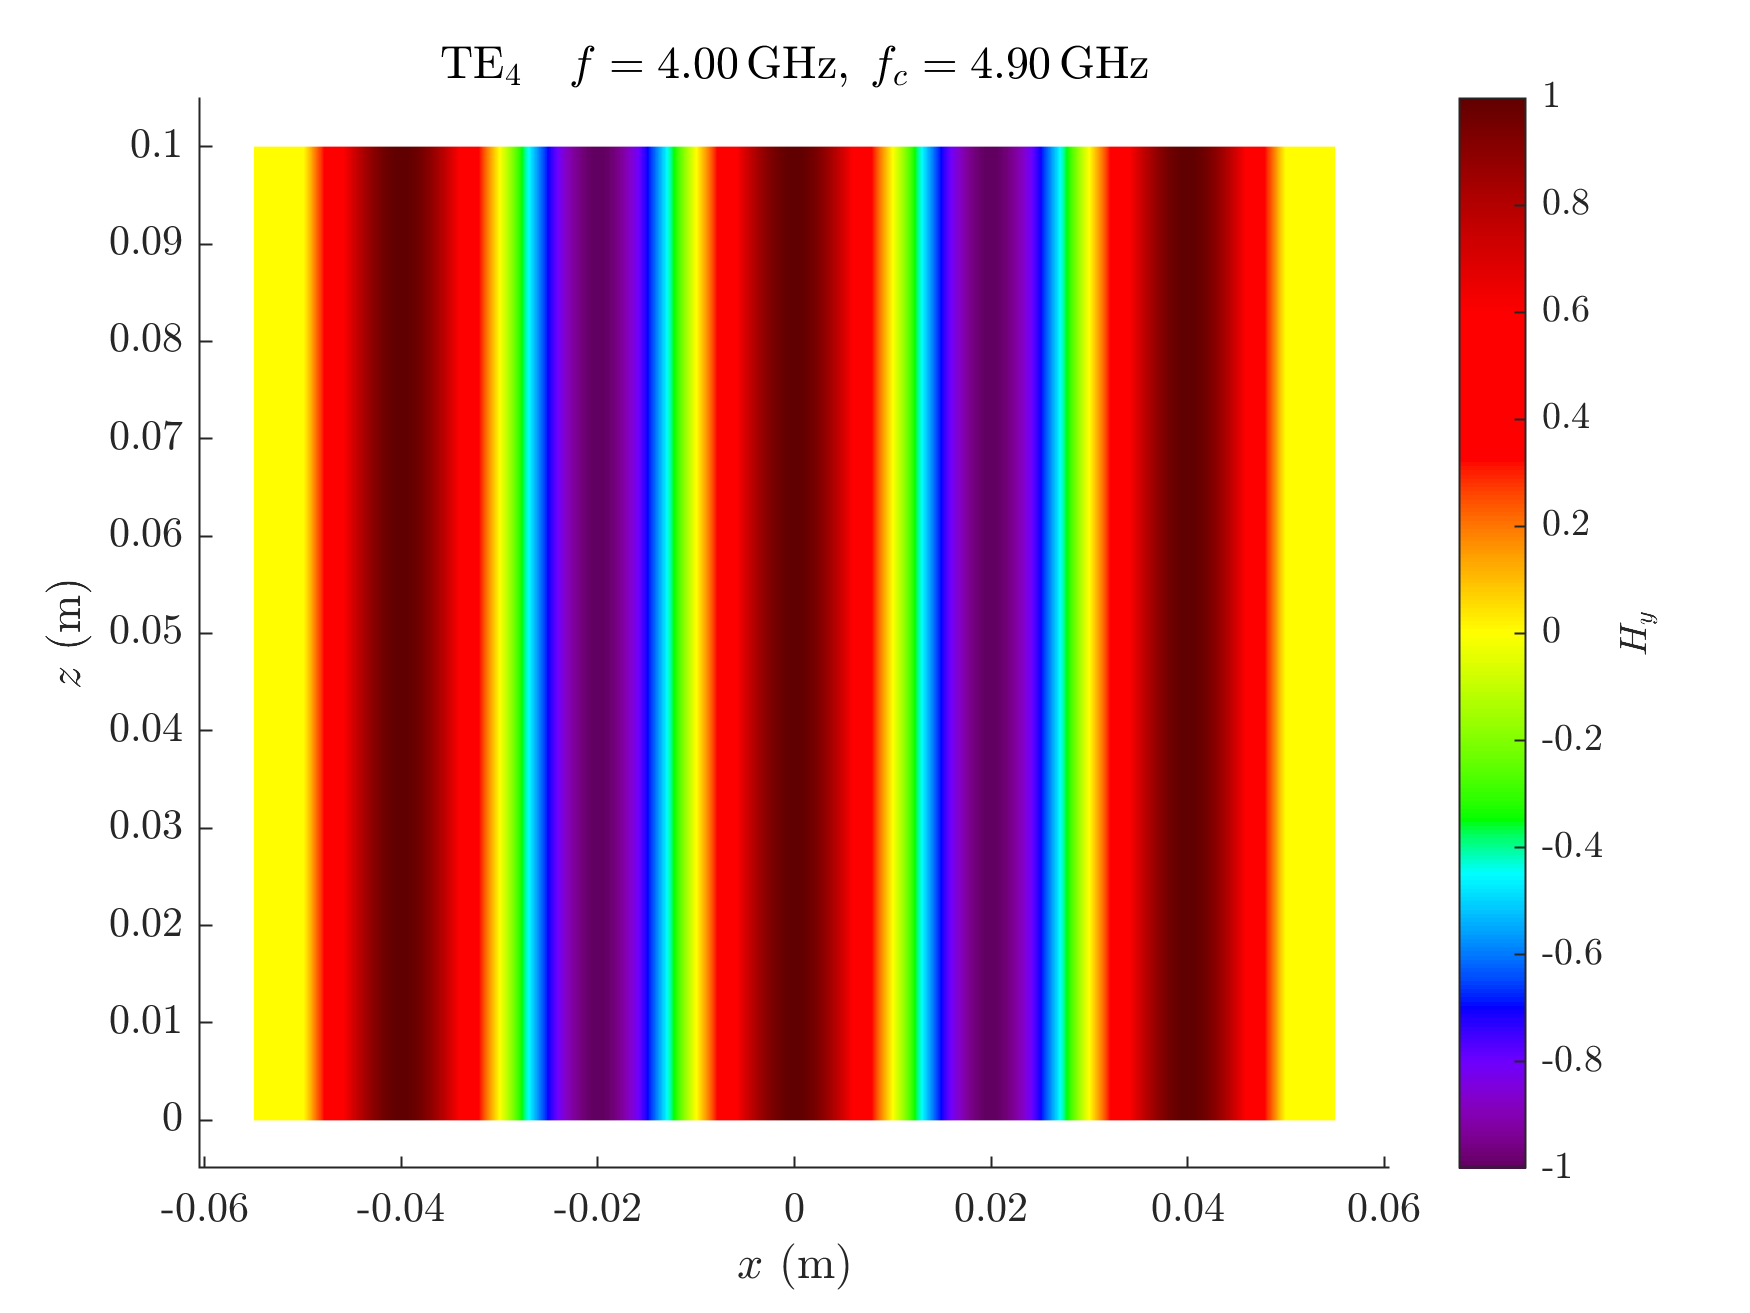
\includegraphics[width=\linewidth]{waveguide_fig/slab_waveguide_te_m4_f4_00ghz.png}
		\caption{TE, \(m=4\), \(f=4.00\ \text{GHz}\)}
		\label{平板波导振幅分布图-TE,m=4,f=4.00GHz}
	\end{subfigure}
	\hfill
	\begin{subfigure}{0.32\textwidth}
		\centering
		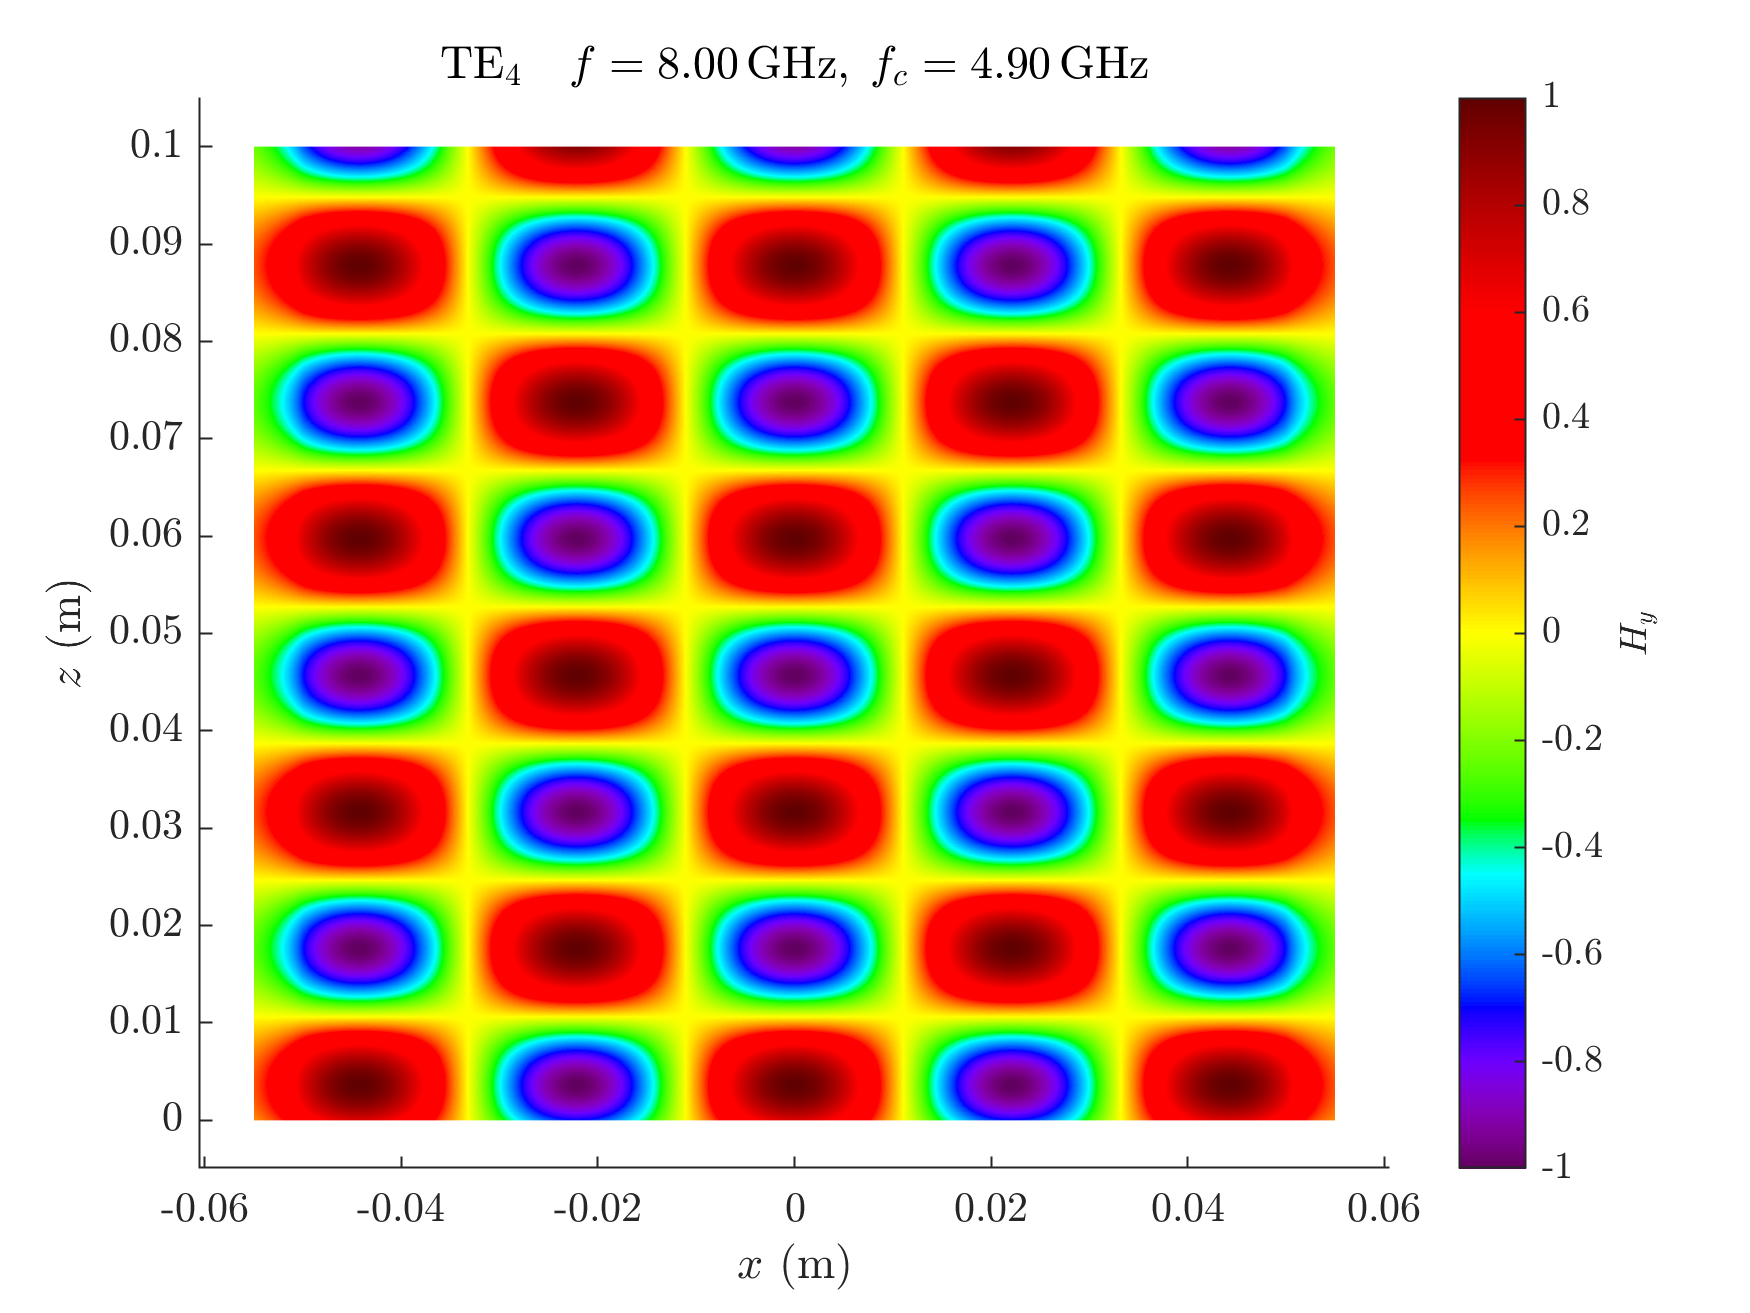
\includegraphics[width=\linewidth]{waveguide_fig/slab_waveguide_te_m4_f8_00ghz.png}
		\caption{TE, \(m=4\), \(f=8.00\ \text{GHz}\)}
		\label{平板波导振幅分布图-TE,m=4,f=8.00GHz}
	\end{subfigure}
	\hfill
	\begin{subfigure}{0.32\textwidth}
		\centering
		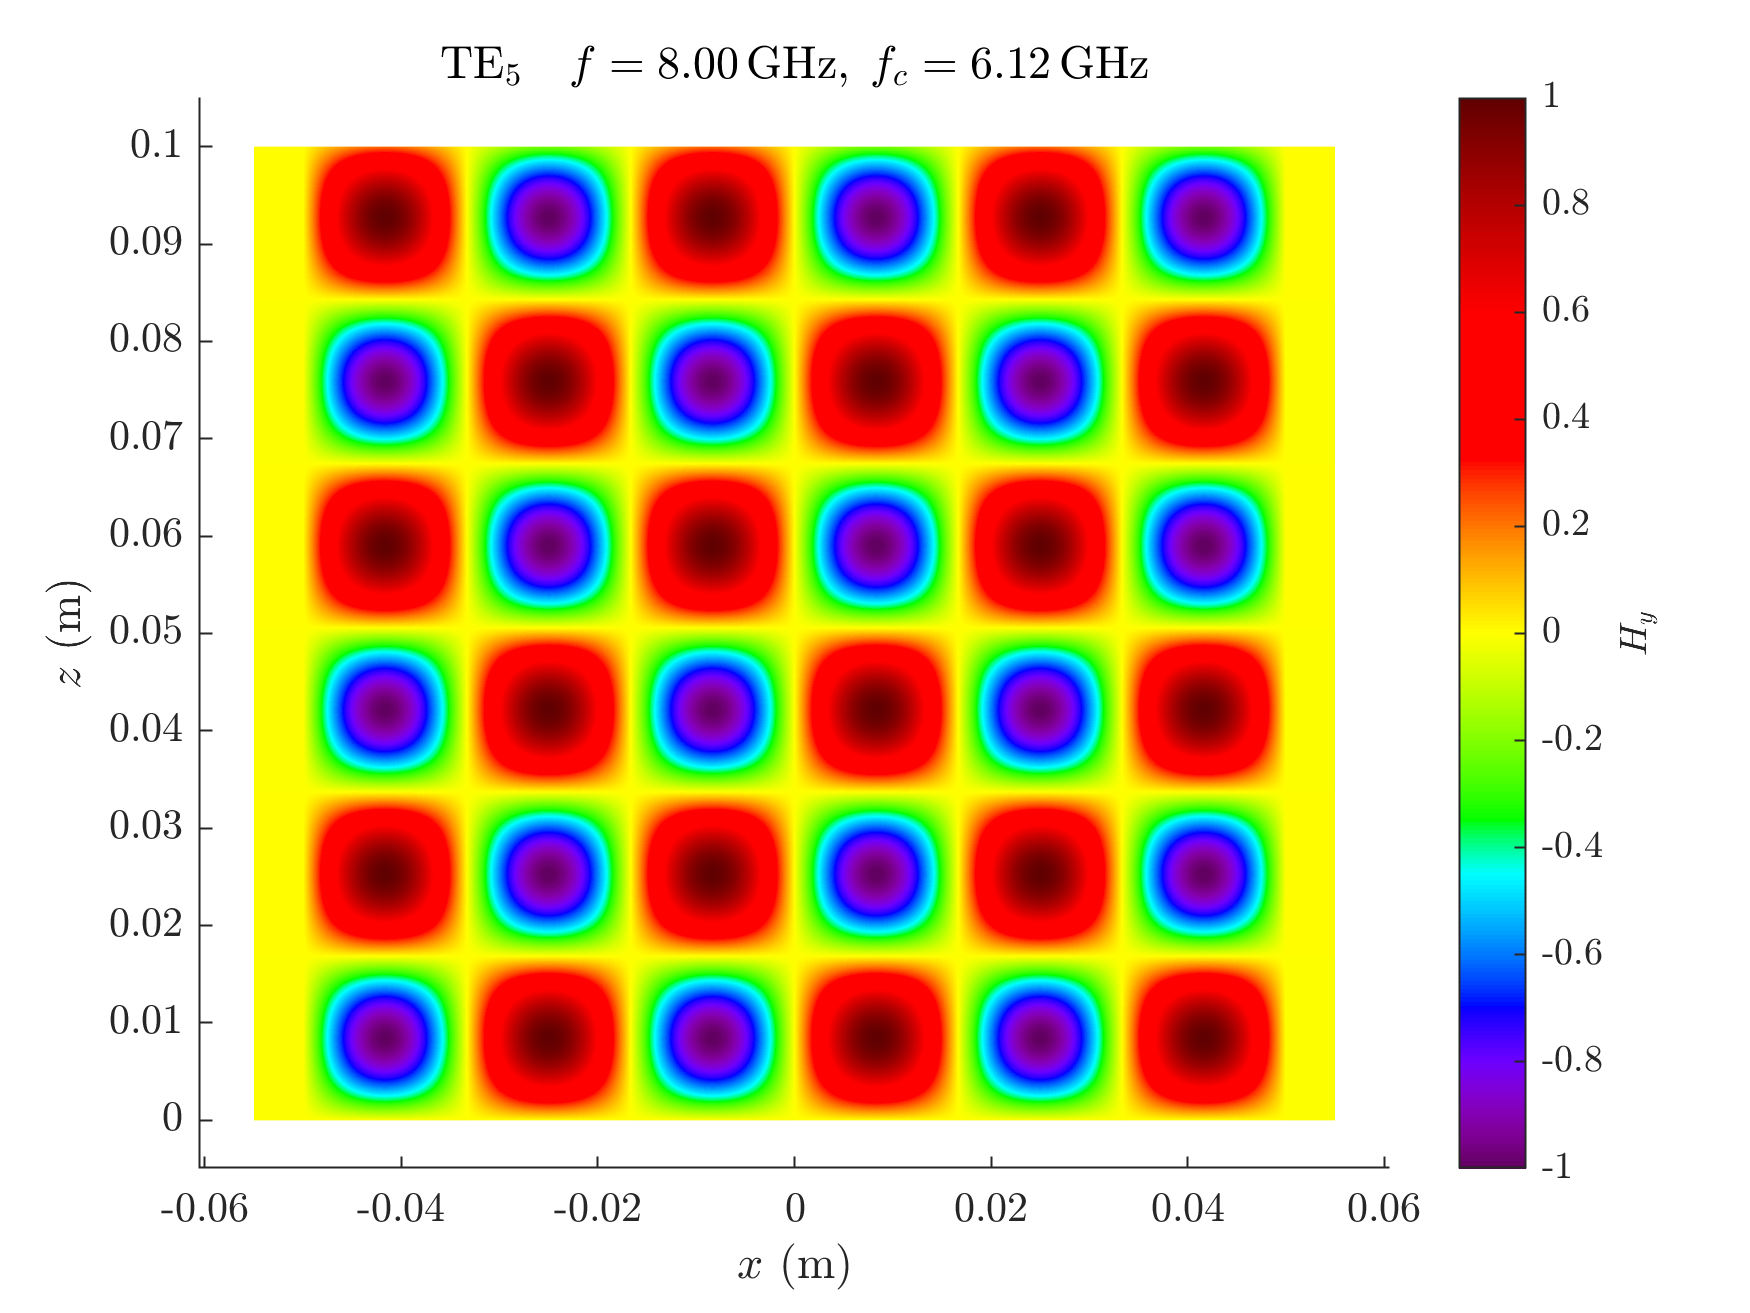
\includegraphics[width=\linewidth]{waveguide_fig/slab_waveguide_te_m5_f8_00ghz.png}
		\caption{TE, \(m=5\), \(f=8.00\ \text{GHz}\)}
		\label{平板波导振幅分布图-TE,m=5,f=8.00GHz}
	\end{subfigure}

	\vspace{1em}

	\begin{subfigure}{0.32\textwidth}
		\centering
		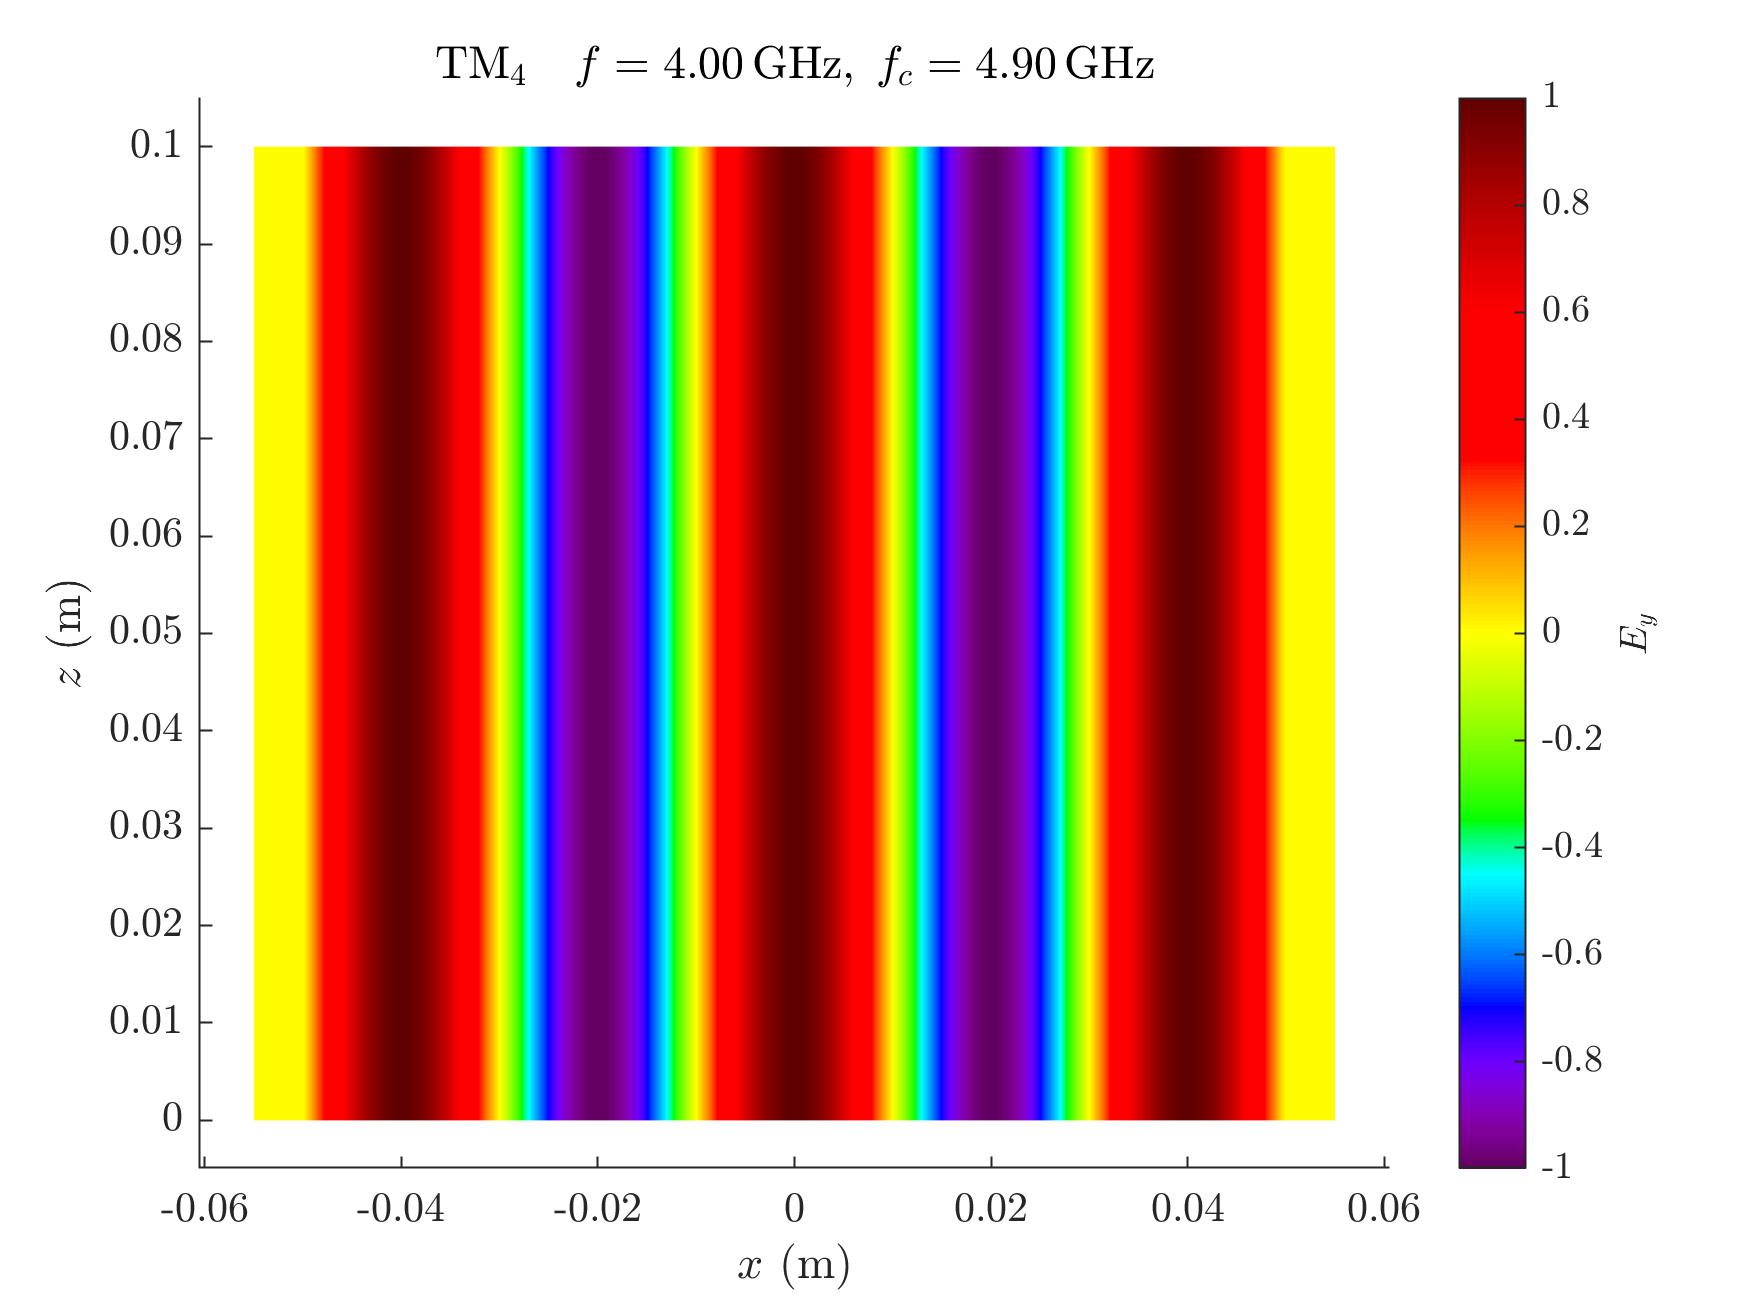
\includegraphics[width=\linewidth]{waveguide_fig/slab_waveguide_tm_m4_f4_00ghz.png}
		\caption{TM, \(m=4\), \(f=4.00\ \text{GHz}\)}
		\label{平板波导振幅分布图-TM,m=4,f=4.00GHz}
	\end{subfigure}
	\hfill
	\begin{subfigure}{0.32\textwidth}
		\centering
		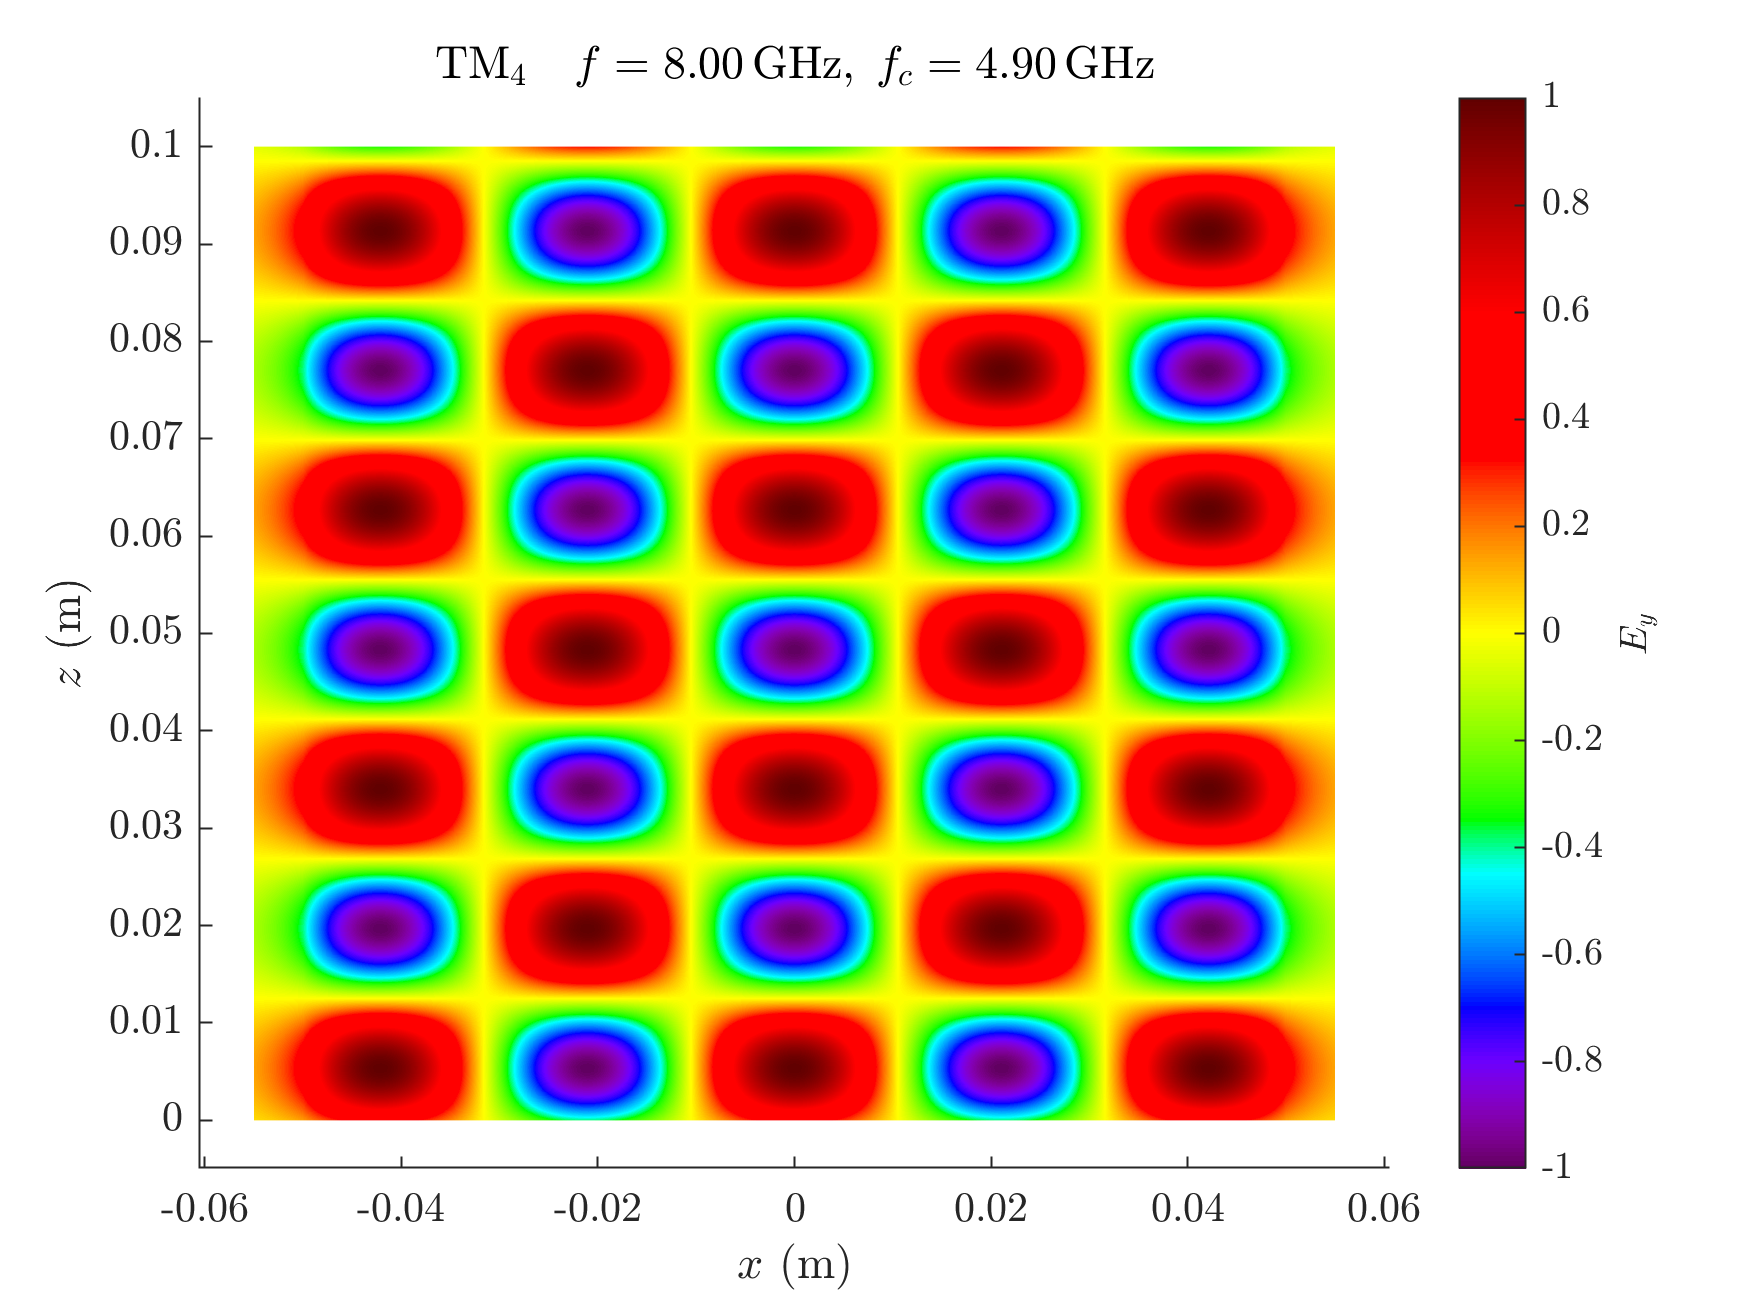
\includegraphics[width=\linewidth]{waveguide_fig/slab_waveguide_tm_m4_f8_00ghz.png}
		\caption{TM, \(m=4\), \(f=8.00\ \text{GHz}\)}
		\label{平板波导振幅分布图-TM,m=4,f=8.00GHz}
	\end{subfigure}
	\hfill
	\begin{subfigure}{0.32\textwidth}
		\centering
		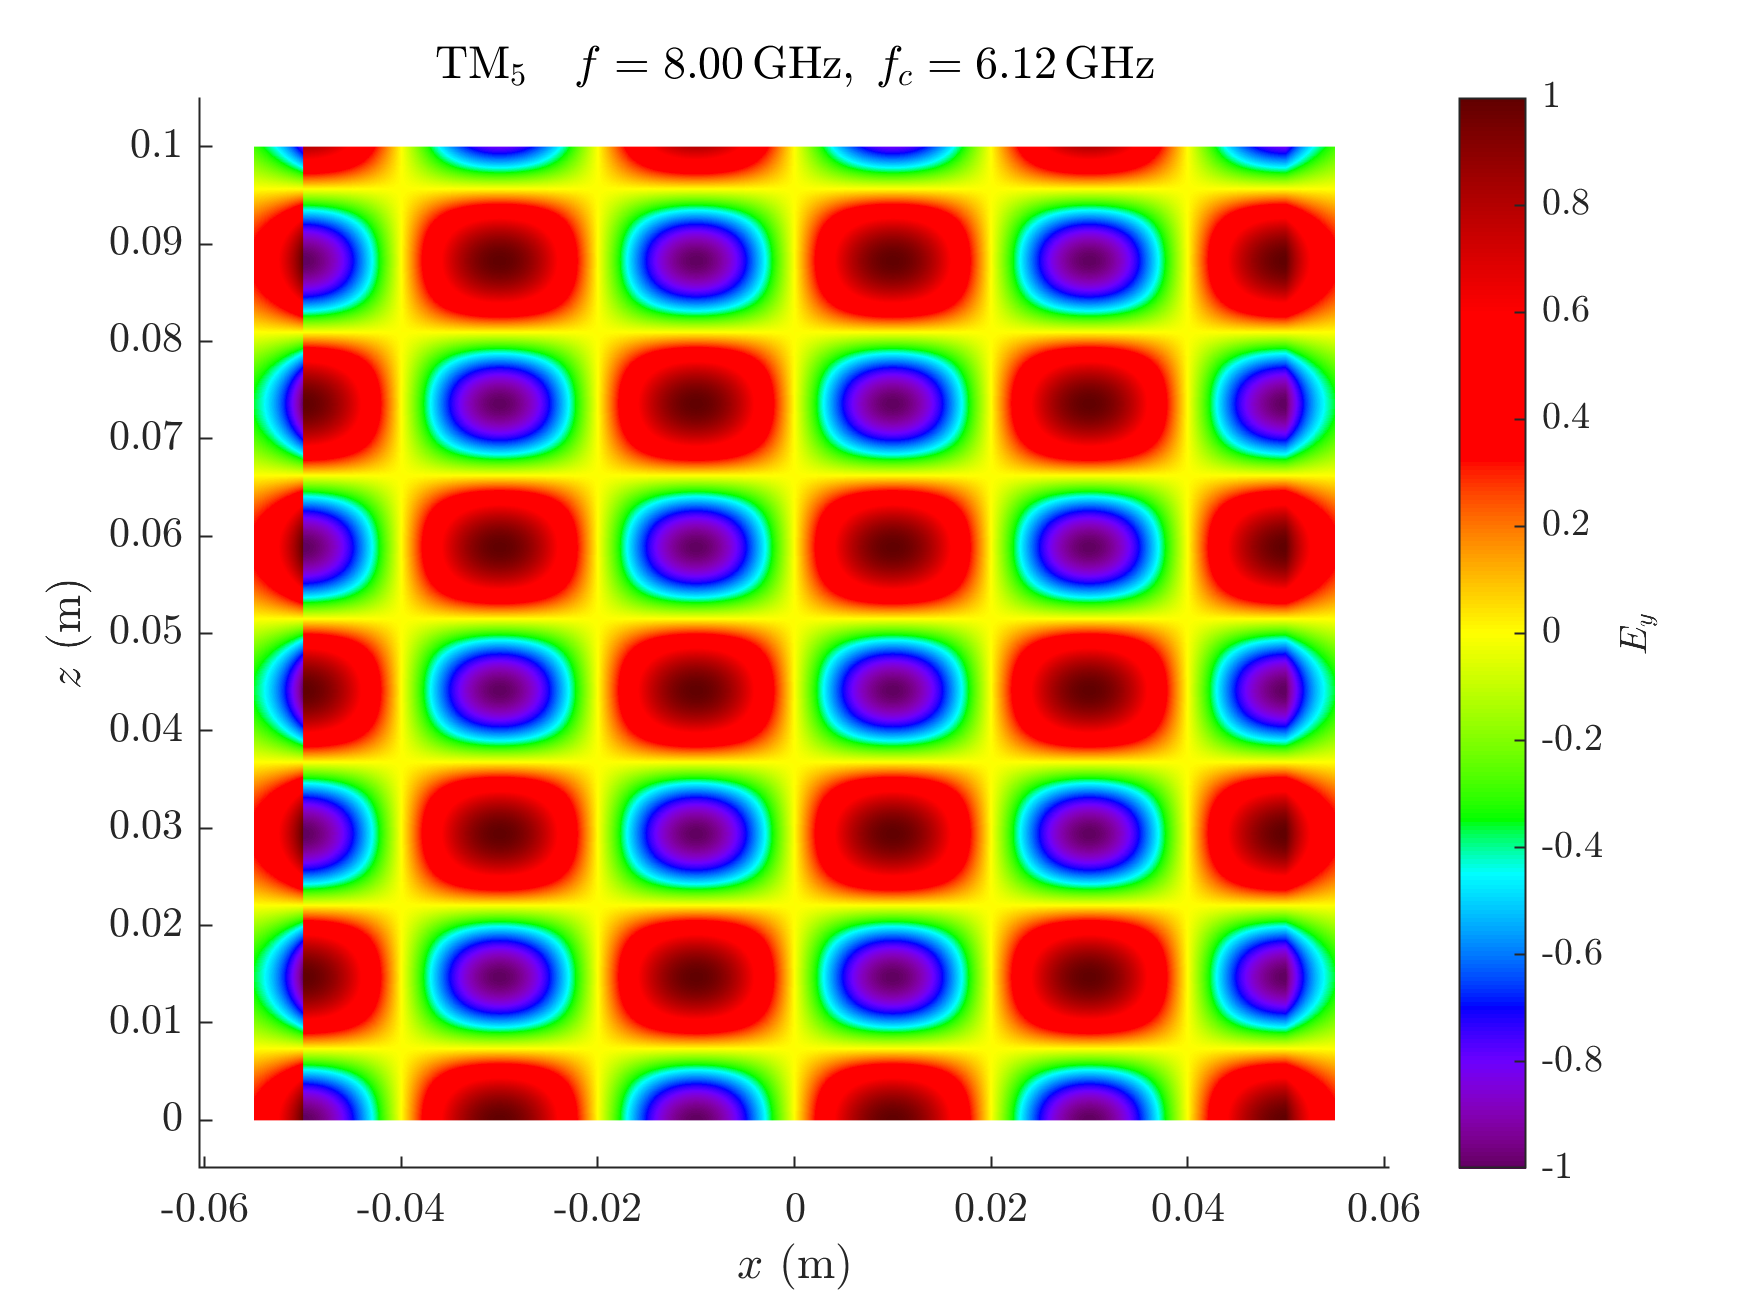
\includegraphics[width=\linewidth]{waveguide_fig/slab_waveguide_tm_m5_f8_00ghz.png}
		\caption{TM, \(m=5\), \(f=8.00\ \text{GHz}\)}
		\label{平板波导振幅分布图-TM,m=5,f=8.00GHz}
	\end{subfigure}
	\caption{平板波导振幅分布图}
	\label{平板波导振幅分布图}
\end{figure}